% Options for packages loaded elsewhere
\PassOptionsToPackage{unicode}{hyperref}
\PassOptionsToPackage{hyphens}{url}
%
\documentclass[
]{book}
\usepackage{amsmath,amssymb}
\usepackage{iftex}
\ifPDFTeX
  \usepackage[T1]{fontenc}
  \usepackage[utf8]{inputenc}
  \usepackage{textcomp} % provide euro and other symbols
\else % if luatex or xetex
  \usepackage{unicode-math} % this also loads fontspec
  \defaultfontfeatures{Scale=MatchLowercase}
  \defaultfontfeatures[\rmfamily]{Ligatures=TeX,Scale=1}
\fi
\usepackage{lmodern}
\ifPDFTeX\else
  % xetex/luatex font selection
\fi
% Use upquote if available, for straight quotes in verbatim environments
\IfFileExists{upquote.sty}{\usepackage{upquote}}{}
\IfFileExists{microtype.sty}{% use microtype if available
  \usepackage[]{microtype}
  \UseMicrotypeSet[protrusion]{basicmath} % disable protrusion for tt fonts
}{}
\makeatletter
\@ifundefined{KOMAClassName}{% if non-KOMA class
  \IfFileExists{parskip.sty}{%
    \usepackage{parskip}
  }{% else
    \setlength{\parindent}{0pt}
    \setlength{\parskip}{6pt plus 2pt minus 1pt}}
}{% if KOMA class
  \KOMAoptions{parskip=half}}
\makeatother
\usepackage{xcolor}
\usepackage{color}
\usepackage{fancyvrb}
\newcommand{\VerbBar}{|}
\newcommand{\VERB}{\Verb[commandchars=\\\{\}]}
\DefineVerbatimEnvironment{Highlighting}{Verbatim}{commandchars=\\\{\}}
% Add ',fontsize=\small' for more characters per line
\usepackage{framed}
\definecolor{shadecolor}{RGB}{248,248,248}
\newenvironment{Shaded}{\begin{snugshade}}{\end{snugshade}}
\newcommand{\AlertTok}[1]{\textcolor[rgb]{0.94,0.16,0.16}{#1}}
\newcommand{\AnnotationTok}[1]{\textcolor[rgb]{0.56,0.35,0.01}{\textbf{\textit{#1}}}}
\newcommand{\AttributeTok}[1]{\textcolor[rgb]{0.13,0.29,0.53}{#1}}
\newcommand{\BaseNTok}[1]{\textcolor[rgb]{0.00,0.00,0.81}{#1}}
\newcommand{\BuiltInTok}[1]{#1}
\newcommand{\CharTok}[1]{\textcolor[rgb]{0.31,0.60,0.02}{#1}}
\newcommand{\CommentTok}[1]{\textcolor[rgb]{0.56,0.35,0.01}{\textit{#1}}}
\newcommand{\CommentVarTok}[1]{\textcolor[rgb]{0.56,0.35,0.01}{\textbf{\textit{#1}}}}
\newcommand{\ConstantTok}[1]{\textcolor[rgb]{0.56,0.35,0.01}{#1}}
\newcommand{\ControlFlowTok}[1]{\textcolor[rgb]{0.13,0.29,0.53}{\textbf{#1}}}
\newcommand{\DataTypeTok}[1]{\textcolor[rgb]{0.13,0.29,0.53}{#1}}
\newcommand{\DecValTok}[1]{\textcolor[rgb]{0.00,0.00,0.81}{#1}}
\newcommand{\DocumentationTok}[1]{\textcolor[rgb]{0.56,0.35,0.01}{\textbf{\textit{#1}}}}
\newcommand{\ErrorTok}[1]{\textcolor[rgb]{0.64,0.00,0.00}{\textbf{#1}}}
\newcommand{\ExtensionTok}[1]{#1}
\newcommand{\FloatTok}[1]{\textcolor[rgb]{0.00,0.00,0.81}{#1}}
\newcommand{\FunctionTok}[1]{\textcolor[rgb]{0.13,0.29,0.53}{\textbf{#1}}}
\newcommand{\ImportTok}[1]{#1}
\newcommand{\InformationTok}[1]{\textcolor[rgb]{0.56,0.35,0.01}{\textbf{\textit{#1}}}}
\newcommand{\KeywordTok}[1]{\textcolor[rgb]{0.13,0.29,0.53}{\textbf{#1}}}
\newcommand{\NormalTok}[1]{#1}
\newcommand{\OperatorTok}[1]{\textcolor[rgb]{0.81,0.36,0.00}{\textbf{#1}}}
\newcommand{\OtherTok}[1]{\textcolor[rgb]{0.56,0.35,0.01}{#1}}
\newcommand{\PreprocessorTok}[1]{\textcolor[rgb]{0.56,0.35,0.01}{\textit{#1}}}
\newcommand{\RegionMarkerTok}[1]{#1}
\newcommand{\SpecialCharTok}[1]{\textcolor[rgb]{0.81,0.36,0.00}{\textbf{#1}}}
\newcommand{\SpecialStringTok}[1]{\textcolor[rgb]{0.31,0.60,0.02}{#1}}
\newcommand{\StringTok}[1]{\textcolor[rgb]{0.31,0.60,0.02}{#1}}
\newcommand{\VariableTok}[1]{\textcolor[rgb]{0.00,0.00,0.00}{#1}}
\newcommand{\VerbatimStringTok}[1]{\textcolor[rgb]{0.31,0.60,0.02}{#1}}
\newcommand{\WarningTok}[1]{\textcolor[rgb]{0.56,0.35,0.01}{\textbf{\textit{#1}}}}
\usepackage{longtable,booktabs,array}
\usepackage{calc} % for calculating minipage widths
% Correct order of tables after \paragraph or \subparagraph
\usepackage{etoolbox}
\makeatletter
\patchcmd\longtable{\par}{\if@noskipsec\mbox{}\fi\par}{}{}
\makeatother
% Allow footnotes in longtable head/foot
\IfFileExists{footnotehyper.sty}{\usepackage{footnotehyper}}{\usepackage{footnote}}
\makesavenoteenv{longtable}
\usepackage{graphicx}
\makeatletter
\def\maxwidth{\ifdim\Gin@nat@width>\linewidth\linewidth\else\Gin@nat@width\fi}
\def\maxheight{\ifdim\Gin@nat@height>\textheight\textheight\else\Gin@nat@height\fi}
\makeatother
% Scale images if necessary, so that they will not overflow the page
% margins by default, and it is still possible to overwrite the defaults
% using explicit options in \includegraphics[width, height, ...]{}
\setkeys{Gin}{width=\maxwidth,height=\maxheight,keepaspectratio}
% Set default figure placement to htbp
\makeatletter
\def\fps@figure{htbp}
\makeatother
\setlength{\emergencystretch}{3em} % prevent overfull lines
\providecommand{\tightlist}{%
  \setlength{\itemsep}{0pt}\setlength{\parskip}{0pt}}
\setcounter{secnumdepth}{5}
\usepackage{booktabs}
\usepackage{amsthm}
\makeatletter
\def\thm@space@setup{%
  \thm@preskip=8pt plus 2pt minus 4pt
  \thm@postskip=\thm@preskip
}
\makeatother
\ifLuaTeX
  \usepackage{selnolig}  % disable illegal ligatures
\fi
\usepackage[]{natbib}
\bibliographystyle{apalike}
\IfFileExists{bookmark.sty}{\usepackage{bookmark}}{\usepackage{hyperref}}
\IfFileExists{xurl.sty}{\usepackage{xurl}}{} % add URL line breaks if available
\urlstyle{same}
\hypersetup{
  pdftitle={MAT 143 E-Coursepack: Brief Calculus},
  pdfauthor={Cheng Peng},
  hidelinks,
  pdfcreator={LaTeX via pandoc}}

\title{MAT 143 E-Coursepack: Brief Calculus}
\author{Cheng Peng}
\date{West Chester University}

\begin{document}
\maketitle

{
\setcounter{tocdepth}{1}
\tableofcontents
}
\begin{Shaded}
\begin{Highlighting}[]
\FunctionTok{install.packages}\NormalTok{(}\StringTok{"bookdown"}\NormalTok{)}
\CommentTok{\# or the development version}
\CommentTok{\# devtools::install\_github("rstudio/bookdown")}
\end{Highlighting}
\end{Shaded}

\hypertarget{introduction}{%
\chapter{Introduction}\label{introduction}}

This \emph{E-Pack} is a self-contained homegrown eBook that contains all topics covered in current MAT 121 at WCU.

The main features of this eBook are

\begin{itemize}
\item
  All technical terms used in this eBook are consistent with those used in the \emph{required} textbook.
\item
  Three formats (PDF, HTML, and EPub) of the E-Pack are accessible from different devices.
\item
  In the HTML version, there are many animated graphics as well as decorative visual aids such as font size, colors, etc. to make some concepts more intuitive.
\item
  The companion course website organizes the weekly topics. It serves as a unique source of all information about this course. The class notes are individual chapters of this eBook.
\end{itemize}

\hypertarget{functions-and-concepts-of-limits}{%
\chapter{Functions and Concepts of Limits}\label{functions-and-concepts-of-limits}}

Here are the basic concepts of functions we learned previously.

\hypertarget{review-of-function}{%
\section{Review of function}\label{review-of-function}}

A \textbf{function} is a \emph{rule} that takes an input, does something to it, and gives a unique corresponding output. If the function name is \(f\), and the input name is \(x\), then the unique corresponding output is called \(f(x)\) (which is read as `\(f\) of \(x\)'). Note that \(f\) and \(f(x)\) are different mathematical expressions:

\begin{enumerate}
\def\labelenumi{\arabic{enumi}.}
\item
  \(f\) is the name of the function;
\item
  \(f(x)\) is the output from the function \(f\) when the input is \(x\).
\end{enumerate}

It is often helpful to think of a function as a `box'. You drop an input at the top, something happens to the input inside the box, and the output drops out the bottom. The box is labeled with the name of the function.

\begin{center}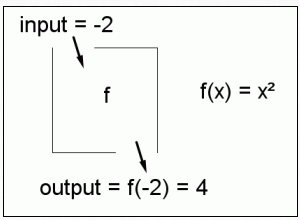
\includegraphics[width=0.3\linewidth]{img01/w01note01-functionDef} \end{center}

Mathematically, a function is an expression that takes input values and produces an output value based on the input value.

\begin{center}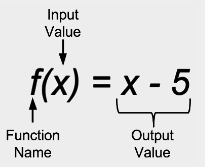
\includegraphics[width=0.15\linewidth]{img01/w01note02-AlgebraicRepresentationFun} \end{center}

The key point in the definition of a function is that \emph{for a given input value, there exists a unique output value}. \textbf{However}, there are functions in which multiple distinct input values could produce the same output value.

\begin{center}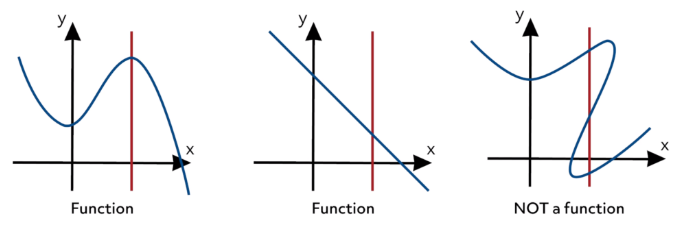
\includegraphics[width=0.65\linewidth]{img01/w01note04-verticalTestFun} \end{center}

\hypertarget{domain-and-range}{%
\subsection{Domain and Range}\label{domain-and-range}}

The \textbf{domain} of a function is the set of all input values. The range of a function is the set of all possible output values.

\begin{center}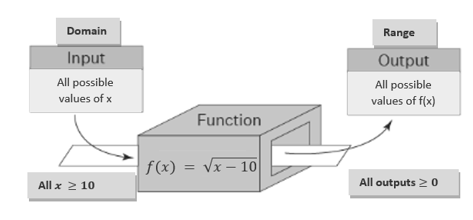
\includegraphics[width=0.55\linewidth]{img01/w01note03-DomainRangeFun} \end{center}

\textbf{Example}: Justify whether each of the following expressions defines a valid function (i.e., pass the vertical test). If it is a valid function, specify the domain and range.

\begin{enumerate}
\def\labelenumi{\arabic{enumi}.}
\item
  \(f(x) = \sqrt{x} + 1/x\).
\item
  \(y = -x^2 + 1\).
\item
  \(y^2 = -x^2 + 1\).
\end{enumerate}

\textbf{Sketch of Solution}: Based on the definition and vertical test, we have the following brief answers to the above questions.

\begin{enumerate}
\def\labelenumi{\arabic{enumi}.}
\tightlist
\item
  It is a valid function. The \textbf{domain} is \(x > 0\). Note that \(x = 0\) is not in the domain. The \textbf{range} is also \(x>0\).
\end{enumerate}

\begin{center}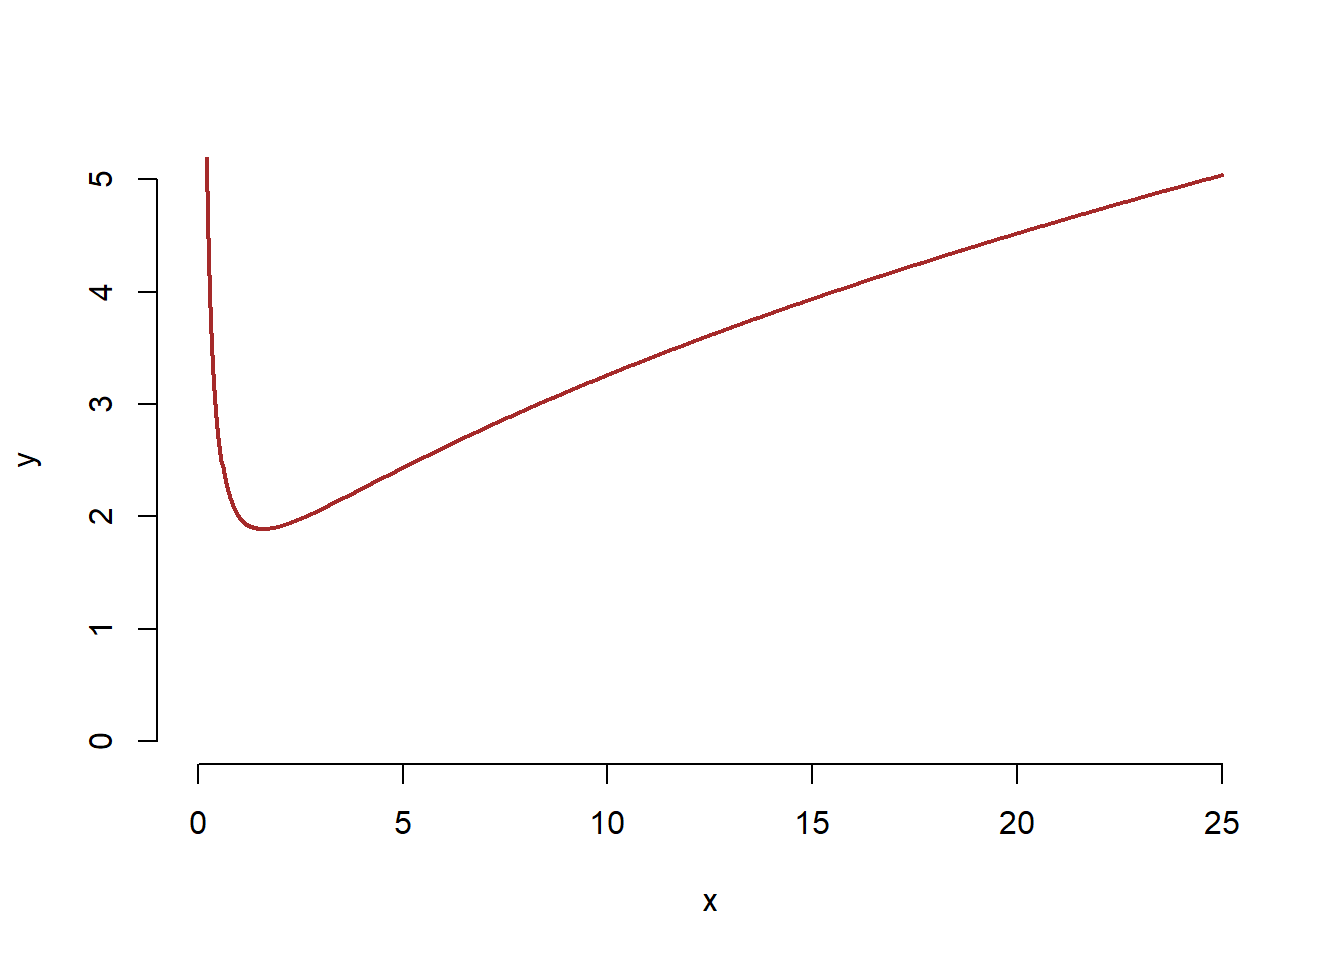
\includegraphics{MAT143EB_files/figure-latex/unnamed-chunk-7-1} \end{center}

\begin{enumerate}
\def\labelenumi{\arabic{enumi}.}
\setcounter{enumi}{1}
\tightlist
\item
  It is also a valid function. The \textbf{domain} is all real numbers. The range
\end{enumerate}

\begin{center}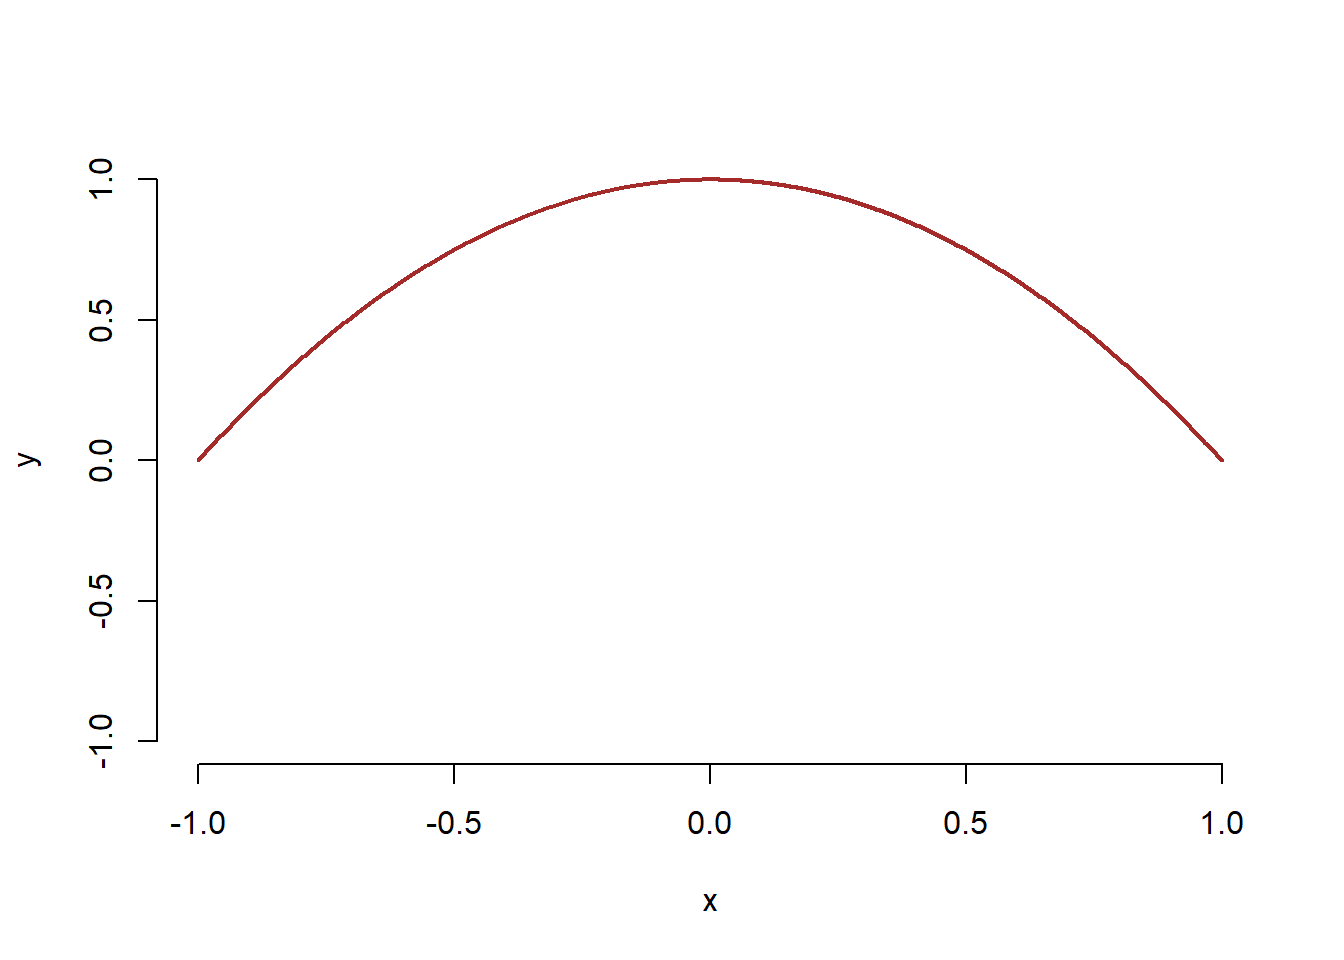
\includegraphics{MAT143EB_files/figure-latex/unnamed-chunk-8-1} \end{center}

\begin{enumerate}
\def\labelenumi{\arabic{enumi}.}
\setcounter{enumi}{2}
\tightlist
\item
  It is not a valid function since fails to pass the vertical line test. In fact, the expression can be rewritten into the following two different forms. \(y = \sqrt{-x^2 + 1}\) (the upper semi-circle) and \(y = -\sqrt{-x^2 +1}\) (the lower semi-circle). Each of the two forms is a valid function. The curve of the expression is given by
\end{enumerate}

\begin{center}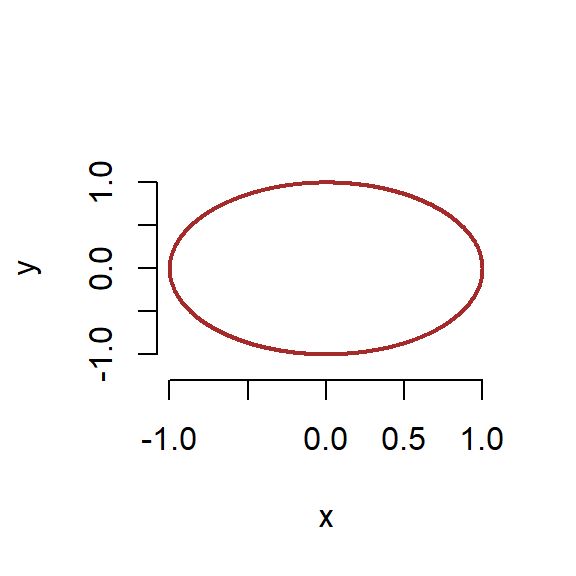
\includegraphics{MAT143EB_files/figure-latex/unnamed-chunk-9-1} \end{center}

\hypertarget{piece-wise-functions}{%
\subsection{Piece-wise Functions}\label{piece-wise-functions}}

Piece-wise functions are common in practice. For example, income tax rates are dependent on the level of income. As an illustrative example, we look at the following function.

\begin{center}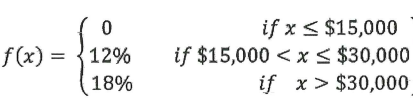
\includegraphics[width=0.4\linewidth]{img01/w01note05-PiecewiseFun} \end{center}

The graph of the above function is given below.

\begin{center}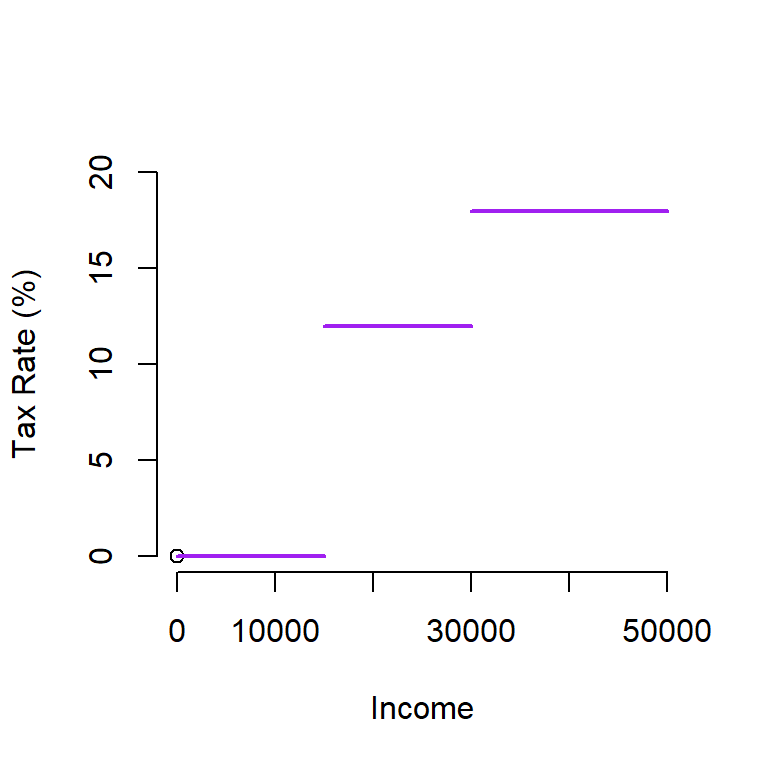
\includegraphics{MAT143EB_files/figure-latex/unnamed-chunk-11-1} \end{center}

The \textbf{domain} of the above function is \(D = [0, \infty]\) (practically, the income cannot be infinity, but mathematically, there is no way to place an upper bound of the income). The \textbf{range} of the above function has only three numbers \(R = \{ 0, 12, 18\}\).

\hypertarget{some-important-functions-and-properties-for-this-course}{%
\subsection{Some Important Functions and Properties for This Course}\label{some-important-functions-and-properties-for-this-course}}

We will only list some functions and properties that are important to this course.

\hypertarget{types-of-functions}{%
\subsubsection{Types of Functions}\label{types-of-functions}}

The function types of functions to be used in this class throughout the semester.

\begin{enumerate}
\def\labelenumi{\arabic{enumi}.}
\item
  \textbf{Polynomial functions}: \(f(x) = a_0 + a_1x + a_2x^2 + \cdots + a_nx^n\) is a n-degree polynomial function. The special cases include \(F9x) = c\) (constant function), \(f(x) = a_0 + a_1x\) (linear function), \(f(x) = a_0 + a_1x + a_2x^2\) (quadratic function), etc.
\item
  \textbf{Power functions}: \(f(x) = x^a\), where \(a\) is any real number (that is called the \textbf{power} of the function). The power function is a special polynomial function that has only one term and the corresponding coefficient is equal to 1. radical root functions such as \(f(x) = \sqrt{x}\) is also power function since they can be expressed as \(f(x) = x^{1/2}\). The reciprocal function \(f(x) = 1/x\) is also a power function since it can be rewritten as \(f(x) = 1/x = x^{-1/2}\).
\item
  \textbf{Rational Functions}: By definition, a rational function is a ratio of two polynomial functions. \(f(x) = p(x)/q(x)\) where \(p(x)\) and \(q(x)\) are both polynomials. \textbf{As an example}, suppose we know that the cost of making a product is dependent on the number of items, \(x\), produced. This is given by \(C(x) = 15000x - 0.1x^2 + 1000\) . If we want to know the average cost for producing \(x\) items, we would divide the cost function by the number of items, \(x\). The average cost function, which yields the average cost per item for \(x\) items produced, is

  \[f(x) = \frac{C(x)}{x} = \frac{15000x - 0.1x^2 + 1000}{x}\]
\item
  \textbf{Logarithmic and Exponential Functions:} For \(a > 0\) and \(a \ne 1\), \(f(x) = \log_a(x)\) is called logarithmic function of \(x\) with \textbf{base} \(a\). \(h(x) = a^x\) is called \textbf{exponential} function with \textbf{base} \(a\). If \(a = e \approx 2.71828\), the corresponding functions are called natural-based logarithmic and exponential functions.
\end{enumerate}

\begin{center}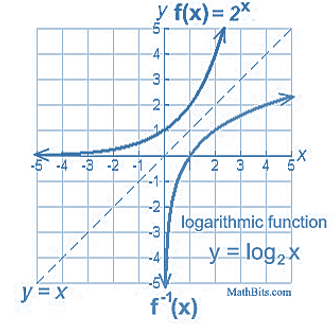
\includegraphics[width=0.4\linewidth]{img01/w01note06-LogExpFun} \end{center}

We can easily find the domains and ranges of the two functions in the above figure. \textbf{Logarithmic function}: \(D_{\text{logarithmic function}} = (0, \infty)\) and \(R_{\text{logarithmic function}} = (-\infty, \infty)\). \textbf{Exponential Function}: \(D_{\text{exponential function}} = (-\infty, \infty)\) and \(R_{\text{exponential function}} = (0, \infty)\).

\textbf{Example}: A local restaurant estimates that weekly sales \(s\) and weekly advertising costs \(x\) (both in dollars) are related by \[s(x) = 14000 - 13000e^{-0.0006t}\].

\hypertarget{monotonic-functions}{%
\subsubsection{Monotonic Functions}\label{monotonic-functions}}

Based on the shape of the curves of functions, we can classify a function in one of the three categories: increasing, decreasing, or neither increasing nor decreasing.

\begin{center}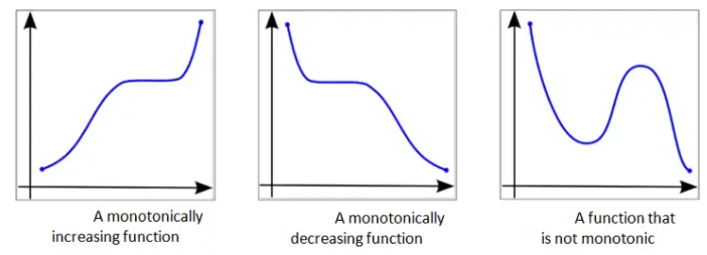
\includegraphics[width=0.6\linewidth]{img01/w01note07-MonotonicFun} \end{center}

Three business functions that we will use frequently are cost, revenue, and profit functions.

\textbf{Example}: Let \(x\) be the number of items manufactured by a factory. We can define the following three frequently used functions.

\begin{enumerate}
\def\labelenumi{\arabic{enumi}.}
\item
  Cost function \(C(x) = 200 + 10x +2x^2\).
\item
  Revenue function \(R(x) = 90 x -2x^2\).
\item
  Profit function \(P(x) = C(x) - R(x) = 80x - 4x^2 - 200\).
\end{enumerate}

The corresponding curves of the above three functions are given in the following figure.

\begin{center}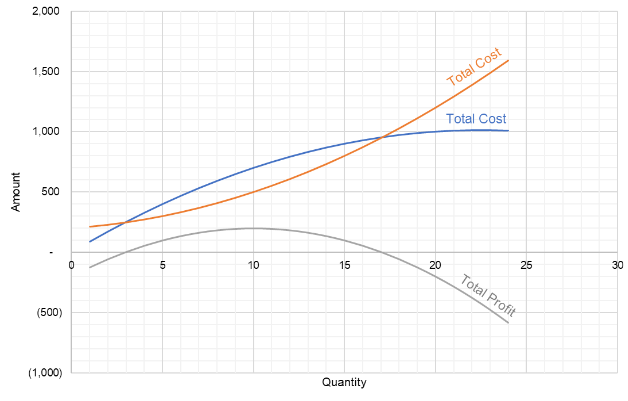
\includegraphics[width=0.6\linewidth]{img01/w01note08-CostRevenueProfitFun} \end{center}

We can see the monotonic patterns of all three functions in the above functions.

\hypertarget{composite-functions}{%
\subsubsection{Composite Functions}\label{composite-functions}}

Given functions \(f:A\to B\) and \(g:B\to C\), the composite function, \(g\circ f\) , which is pronounced as \(g\) circle \(f\), is defined as \[g\circ f:A→C,(g\circ f)(x)=g(f(x))\].

\begin{center}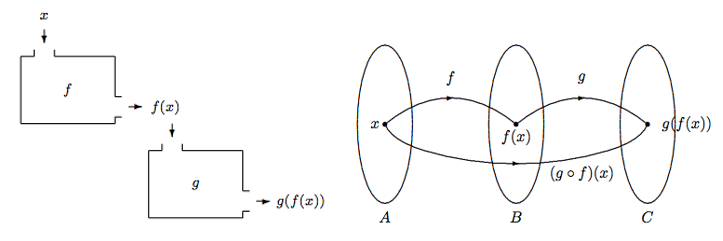
\includegraphics[width=0.8\linewidth]{img01/w01note09-CompositeFun} \end{center}

\textbf{Example}: Assume \(f,g:R \to R\) are defined as \(f(x)=x^2\), and \$ g(x)=3x+1\$. Find \(f\circ g\) and \(g\circ f\).

\textbf{Solution}: Using the definition, we have

\(f\circ g (x) = f(g(x)) = [g(x)]^2= (3x + 1)^2\),

\(g\circ f (x) = g(f(x)) = 3\times f(x) + 1 = 3x^2 + 1\).

In general, \(f\circ g \ne g \circ f\).

\hypertarget{inverse-functions}{%
\subsubsection{Inverse Functions}\label{inverse-functions}}

Let \(f\) and \(g\) be two functions such that

\begin{enumerate}
\def\labelenumi{\arabic{enumi}.}
\item
  \(f\circ g(x) = f(g(x)) = x\), for every \(x\) in the domain of \(g\)
\item
  \(g\circ f(x) = g(f(x)) = x\), for every \(x\) in the domain of \(f\),
\end{enumerate}

then the function \(g\) is said to be the inverse of the function \(f\) and is denoted \(f^{-1}\). The domain of \(f\) is equal to the range of \(f^{-1}\) and the range of \(f\) is the domain of \(f^{-1}\).

The relationship between a function \(f(x)\) and its inverse \(f^{-1}(x)\) is graphically characterized in the following figure.

\begin{center}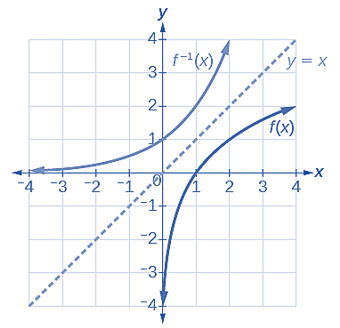
\includegraphics[width=0.45\linewidth]{img01/w01note10-InverseFun} \end{center}

We can see from the above figure that \(f(x)\) and \(f^{-1}(x)\) are symmetric with respect to \(y = x\). Since both \(f(x)\) and \(f^{-1}(x)\) MUST pass the vertical test, therefore, the inverse of \(f(x)\) exists if and only if it is strictly monotonic.

The following example demonstrates the steps for finding an inverse function.

\textbf{Example}: Find the inverse function of \(f(x) = 2x^3 + 1\).

\textbf{Solution}: The detailed steps for finding the inverse function are outlined below.

\begin{center}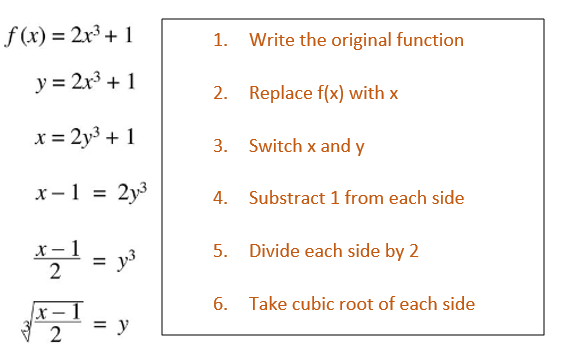
\includegraphics[width=0.55\linewidth]{img01/w01note11-FindingInverseFun} \end{center}

\hypertarget{concepts-of-limits}{%
\section{Concepts of Limits}\label{concepts-of-limits}}

We first introduce the concept of limit intuitively before presenting the technical steps for finding the limit of a given function at a given point.

\hypertarget{definition-of-limits-on-the-number-line}{%
\subsection{Definition of Limits on the number line}\label{definition-of-limits-on-the-number-line}}

\textbf{Definition}: A quantity \(L\) is the limit of a function \(f(x)\) as \(x\) approaches \(a\) if, as the input values of \(x\) approach \(a\) (but do not equal \(a\)), the corresponding output values of \(f(x)\) get closer to \(L\). Note that the value of the limit is not affected by the output value of \(f(x)\) at \(a\). Both \(a\) and \(L\) must be real numbers. We write it as \[
\lim_{x \to a} f(x) = L.
\]

Note that \(x \to a\) means \emph{approaches} \(a\). There are two different ways to approach \(a\): from the left-hand and right-hand. This leads to the definition of a one-sided limit.

\textbf{Left Limit (also called Left-hand Limit)}: The of a function \(f(x)\) as \(x\) approaches \(a\) from the \textbf{left} is equal to \(L\), denoted by
\[
\lim_{x \to a^-} f(x) = L.
\]

\textbf{Left Limit (also called Left-hand Limit)}: The of a function \(f(x)\) as \(x\) approaches \(a\) from the \textbf{right} is equal to \(L\), denoted by \[
\lim_{x \to a^+} f(x) = L.
\]

The following figure illustrates the above three definitions.

\begin{center}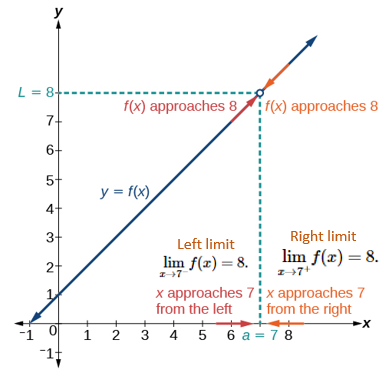
\includegraphics[width=0.55\linewidth]{img01/w01note11-LeftRightLimits} \end{center}

\hypertarget{existence-of-limit}{%
\subsection{Existence of Limit}\label{existence-of-limit}}

If both left and right limits exist and are equal at \(a\), the limit of the function exists at \(a\) and is equal to both one-sided limits. The above figure illustrates the existence of a limit.

\begin{center}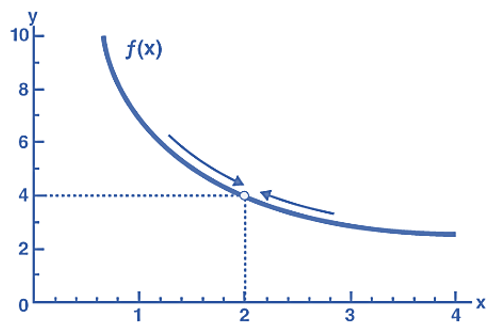
\includegraphics[width=0.55\linewidth]{img01/w01note13-ExistenceLimits} \end{center}

The next animated graph illustrates the process of obtaining the limit.

\hfill\break

\url{https://github.com/pengdsci/MAT143/raw/main/w01/w01-LimitAtAPoint.gif}

\hypertarget{graphical-analysis-of-limits}{%
\subsection{Graphical Analysis of Limits}\label{graphical-analysis-of-limits}}

We can use graphs to identify the limit of a function \(f(x)\) at \(a\).

\hypertarget{non-existence-of-limits}{%
\subsubsection{Non-existence of Limits}\label{non-existence-of-limits}}

If the left limit and right limit exist (i.e., not equal to infinity) but are not equal, the limit of the function does not exist. If both one-sided limits exist and are equal, the limit of the function exists.

\begin{center}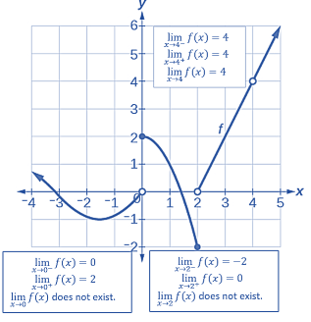
\includegraphics[width=0.45\linewidth]{img01/w01note12-FindingLimitsGraphically} \end{center}

\hfill\break

An animated graph that shows the case of unequal onesided limits is given below.

\url{https://github.com/pengdsci/MAT143/raw/main/w01/w01-LeftRightLimits-Unequal.gif}

\hfill\break

\hypertarget{infinite-limits}{%
\subsubsection{Infinite Limits}\label{infinite-limits}}

When one or both one-sided limits are equal to infinity (regardless of positive or negative infinity), the limit of the function does not exist.

\begin{center}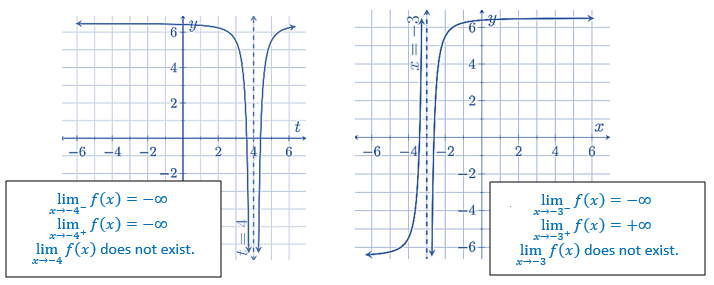
\includegraphics[width=0.95\linewidth]{img01/w01note14-NonExistenceInfiniteLimits} \end{center}

\hfill\break

The following animated graph shows the limiting process.

\hfill\break

\url{https://github.com/pengdsci/MAT143/raw/main/w01/w01-InfiniteLimitAtAPoint.gif}

\hypertarget{limit-when-x-approaches-infty}{%
\subsubsection{\texorpdfstring{Limit When \(x\) Approaches \(\infty\)}{Limit When x Approaches \textbackslash infty}}\label{limit-when-x-approaches-infty}}

When \(x\) goes either positive infinity or negative infinity, the resulting exists if and only if the limit is finite. Otherwise, the limit does not exist.

\begin{center}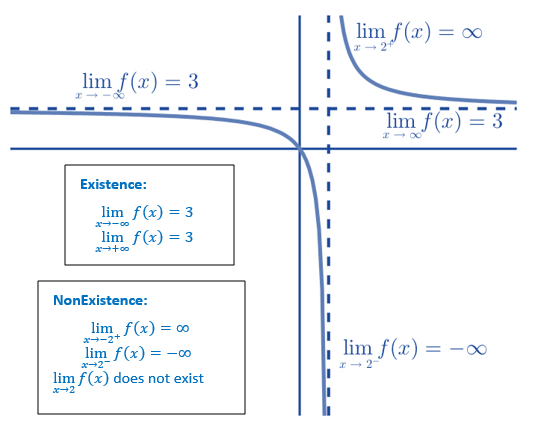
\includegraphics[width=0.55\linewidth]{img01/w01note15-LimitsWinfinity} \end{center}

\hfill\break

The next animated graph depicts the limiting process of the general case.
\url{https://github.com/pengdsci/MAT143/raw/main/w01/w01-LimitAtInfinity.gif}

\hypertarget{calculating-limits}{%
\subsection{Calculating Limits}\label{calculating-limits}}

We have described how to find the limit of a function at a given point graphically. Next we introduce how to find limit algebraically. The basic method is \textbf{substitution}. The following chart outlines the workflow in calculating the limit of a given function at a given value of the independent variable.

\begin{center}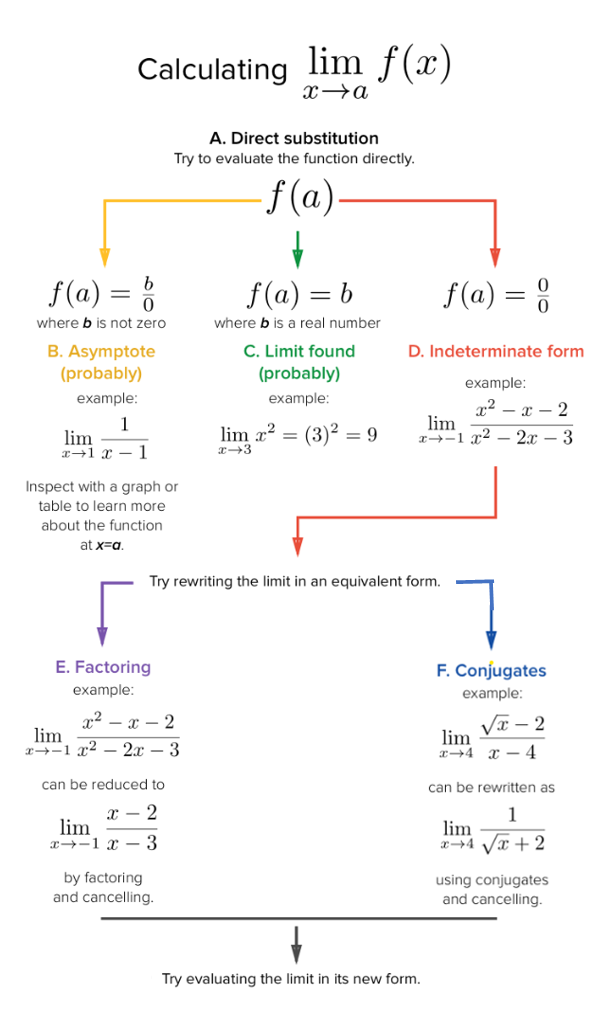
\includegraphics[width=0.75\linewidth]{img01/w01-CalculateLimit} \end{center}

\hypertarget{properties-of-limits}{%
\subsection{Properties of Limits}\label{properties-of-limits}}

\hypertarget{sum-rule}{%
\subsubsection{Sum Rule}\label{sum-rule}}

This rule states that the limit of the sum of two functions is equal to the sum of their limits:
\[
\lim_{x\to a}[f_1(x) + f_2(x) ] = \lim_{x\to a}f_1(x) + \lim_{x\to a}f_2(x).
\]

\hypertarget{constant-function-rule}{%
\subsubsection{Constant Function Rule}\label{constant-function-rule}}

The limit of a constant function is the constant: \[\lim_{x\to a} C = C.\]

\hypertarget{constant-multiple-rule}{%
\subsubsection{Constant Multiple Rule}\label{constant-multiple-rule}}

The limit of constant times a function is equal to the product of the constant and the limit of the function: \[
\lim_{x\to a}Cf(x) = k\lim_{x\to a}f(x).
\]

\hypertarget{product-rule}{%
\subsubsection{Product Rule}\label{product-rule}}

This rule says that the limit of the product of two functions is the product of their limits (if they exist): \[
\lim_{x\to a}[f_1(x)f_2(x)] = \lim_{x\to a}f_1(x)\lim_{x\to a}f(x)
\]

\hypertarget{quotient-rule}{%
\subsubsection{Quotient Rule}\label{quotient-rule}}

The limit of the quotient of two functions is the quotient of their limits, provided that the limit in the denominator function is not zero:
\[
\lim_{x\to a}\frac{f(x)}{g(x)} = \frac{\lim_{x\to a}f(x)}{\lim_{x\to a}g(x)}.
\]

\hypertarget{power-rule}{%
\subsubsection{Power Rule}\label{power-rule}}

For any real number \(p\),
\[
\lim_{x\to a}[f(x)]^p = [\lim_{x\to a}f(x)]^p.
\]
In particular,

\[
\lim_{x\to a}\sqrt[p]{f(x)} = \sqrt[p]{\lim_{x\to a}f(x)}.
\]

\hypertarget{algebraic-calculation-of-limits-by-examples}{%
\subsection{Algebraic Calculation of Limits by Examples}\label{algebraic-calculation-of-limits-by-examples}}

\textbf{Example 1}: Compute the value of the following limit
\[
\lim_{x\to -2}(3x^2 + 5x -9).
\]

\textbf{Solution}:

\[
\lim_{x\to -2}(3x^2 + 5x -9) = 3[\lim_{x\to -2} x]^2 + 5\lim_{x\to -2}x - \lim_{x\to -2}9 = 3\times (-2)^2 + 5(-2) - 9 = -7.
\]

\textbf{Example 2}: Evaluate the following limit.

\[
\lim_{x\to 1}\frac{6-3x+10x^2}{-2x^4+7x^3+1}.
\]
\textbf{Solution}: Using properties of limit, we have

\[
\lim_{x\to 1}\frac{6-3x+10x^2}{-2x^4+7x^3+1}=\frac{\lim_{x\to 1}[6-3x+10x^2]}{\lim_{x\to 1}[-2x^4+7x^3+1]}=\frac{6-3(1)+10(1)^2}{-2(1)^4+7(1)^3+1}=\frac{13}{6}.
\]

\textbf{Example 3} Find the limit

\[
\lim_{x\to 9}\frac{4x^2}{1+\sqrt{x}}.
\]

\textbf{Solution}: Using the properties of limits (the sum rule, the power rule, and the quotient rule), we get \[
\lim_{x\to 9}\frac{4x^2}{1+\sqrt{x}}=\frac{\lim_{x\to 9}(4x^2)}{\lim_{x\to 9}(1+\sqrt{x})} = \frac{4\lim_{x\to 9}(x^2)}{(\lim_{x\to 9}1+\lim_{x\to 9}\sqrt{x})} = \frac{4\times 9^2}{(1+\sqrt{9})} = 81.
\]

\textbf{Example 4}: Suppose that \(\lim_{x\to 1}f(x) = 2\) and \(\lim_{x \to 1}g(x) = 3\). Calculate the limit
\[
 \frac{g(x) - 3f(x)}{f^2(x) + g(x)}
 \]

\textbf{Solution}: Using the properties of limit, we have
\[
\lim_{x\to 1} \frac{g(x) - 3f(x)}{f^2(x) + g(x)} =  \frac{\lim_{x\to 1}[g(x) - 3f(x)]}{\lim_{x\to 1}[f^2(x) + g(x)]} = \frac{\lim_{x\to 1}g(x) - 3\lim_{x\to 1}f(x)}{[\lim_{x\to 1}f(x)]^2 + \lim_{x\to 1}g(x)} = -\frac{3}{7}.
\]

\hypertarget{average-rate-of-change.}{%
\section{Average Rate of Change.}\label{average-rate-of-change.}}

Often times we are not just interested in a function \(f(x)\) itself but also in how \(f(x)\) changes. To be specific, we may be interested in how much the function changed per unit, on average, over an interval.

\hypertarget{average-rate-of-change-of-a-function-over-an-interval}{%
\subsection{Average rate of change of a function over an interval}\label{average-rate-of-change-of-a-function-over-an-interval}}

\textbf{Average rate of change of a function} \(f(x)\) over an interval {[}\(a, b\){]} for \(a \ne b\) is defined to be \[
\frac{f(b)-f(a)}{b-a}
\] The geometric interpretation of the average rate of change is the slope of the secant line defined based on the interval.

\begin{center}\includegraphics[width=0.45\linewidth]{img01/w01note16-SecantLineSlope} \end{center}

\textbf{Example}: According to Google Maps, it's about 33 miles from WCU to the Independent Hall in Philadelphia. If Kevin made this trip in 45 minutes, what was his average rate of travel during the trip?

\begin{center}\includegraphics[width=0.65\linewidth]{img01/w01note17-RateChangeDistance} \end{center}

\textbf{Solution}: Let \(t\) be the driving time and \(f(t)\) the driving distance (that is a function of time \(t\)). We set \(t=0\) at the starting point, i.e., \(f(0)=0\). Since it takes 0.75 hours to drive to the destination, this means \(f(0.75) = 33\). Now based on the definition of \textbf{the rate of change of the distance function} \(f(t)\) on interval \([0, 0.75]\), we have \[
V = \frac{f(0.75) - f(0)}{0.75-0} = \frac{33-0}{0.75-0} = \frac{33}{0.75} = 44.
\] The rate of change is 44 miles per hour.

\textbf{Example}: In 1998, Linda purchased a house for \$144,000. In 2009, the house was worth \$245,000. Find the average annual rate of change in dollars per year in the value of the house. Round your answer to the nearest dollar.

\textbf{Solution}: Since house prices (\(P\)) change over time (\(t\)), therefore, house price is a function of time \(P(t)\). The objective is to find the annual rate of change of the house price. It is natural to use the year as the time variable \(t\) and set \(f(1998) = 144000\) and \(f(2009) = 245000\). Then the annual rate of change is \[
\frac{f(2009) - f(1998)}{2009 - 1998} = \frac{245000-144000}{2009-1998} \approx 9182.
\]

The annual rate of change is approximately equal to \$9182.

\hypertarget{difference-quotient}{%
\subsection{Difference quotient}\label{difference-quotient}}

The difference quotient of a (single variable) function is usually the name for the following expression

\[
\frac{f(x+h)-f(x)}{h}.
\]

This is a variation of the formula of the rate of change

\[
\frac{f(b)-f(a)}{b -a}
\]

where \(a = x\) and \(h = b -a\). We usually assume that \(h\) is close to zero. Without loss of generality, \(h\) is usually assumed to be a small positive number close to zero.

The notation of the difference quotient is easy to use to describe the derivative of a function.

\textbf{Example}: Find the difference quotient of \(f(x) = x^2 + 4x -6\).

\textbf{Solution}: Using the definition of the difference of quotient, we have
\[
\frac{f(x+h)-f(x)}{h} = \frac{[(x+h)^2 + 4(x+h) -6]-[x^2+4x-6]}{h}=\frac{2hx+h^2+4h}{h}=2x+h+4.
\]

\textbf{Example}: Find the difference quotient of \(f(x) = \sqrt{x}\).

\textbf{Solution}: Using the formula of the difference quotient, we have
\[
\frac{\sqrt{x+h}-\sqrt{x}}{h} = \frac{(\sqrt{x+h}-\sqrt{x})(\sqrt{x+h}+\sqrt{x})}{h(\sqrt{x+h}-\sqrt{x})} = \frac{(x+h)-x}{{h(\sqrt{x+h}+\sqrt{x})}} = \frac{1}{\sqrt{x+h}+\sqrt{x}}.
\]

\textbf{Example}: Let \(D\) be on the elasticity of demand that is generally defined in the following
\[
D = \frac{tC}{P + t}
\]

where \(P,t, C\) are respectively price, tax, and constant. We are interested in the effect of the tax change on demand by looking at the difference quotient.

\textbf{Solution}: By the definition of \textbf{difference quotient}, we have
\[
\frac{D(t+h) - D(t)}{h} = \frac{\frac{(t+h)C}{P+(t+h)}-\frac{tC}{P+t}}{h} = \frac{(t+h)C}{h(P+t+h)}-\frac{tC}{h(P+t)}
\]

\hypertarget{exercises}{%
\section{Exercises}\label{exercises}}

\begin{enumerate}
\def\labelenumi{\arabic{enumi}.}
\item
  A bakery has the following pricing for large orders of cupcakes. The first 100 cupcakes of any order cost \$2.00 each. Each of the next 150 cupcakes only cost \$1.75. And each cupcake ordered in excess of 250 costs \$1.25. Write the expression of the function and specify the domain and the range of the function respectively.
\item
  A rental home on Airbnb rents for \$100 a night for the first three nights, \$90 a night for the next three nights, and \$80 a night for each remaining night. The total cost \(T\) is a function of the number of nights \(x\) that a guest stays. Write the piece-wise
\end{enumerate}

\hypertarget{average-rate-of-change-of-a-function}{%
\chapter{Average Rate of Change of A Function}\label{average-rate-of-change-of-a-function}}

We first review definitions and properties of limits and then introduce the definition of average rate of change of a given function and its technical calculation and geometry.

\hypertarget{review-properties-of-limits}{%
\section{Review: Properties of Limits}\label{review-properties-of-limits}}

We have described how to find the limit of a function at a given point graphically. Next we introduce how to find limit algebraically. The basic method is \textbf{substitution}. The following chart outlines the workflow in calculating the limit of a given function at a given value of the independent variable.

\begin{center}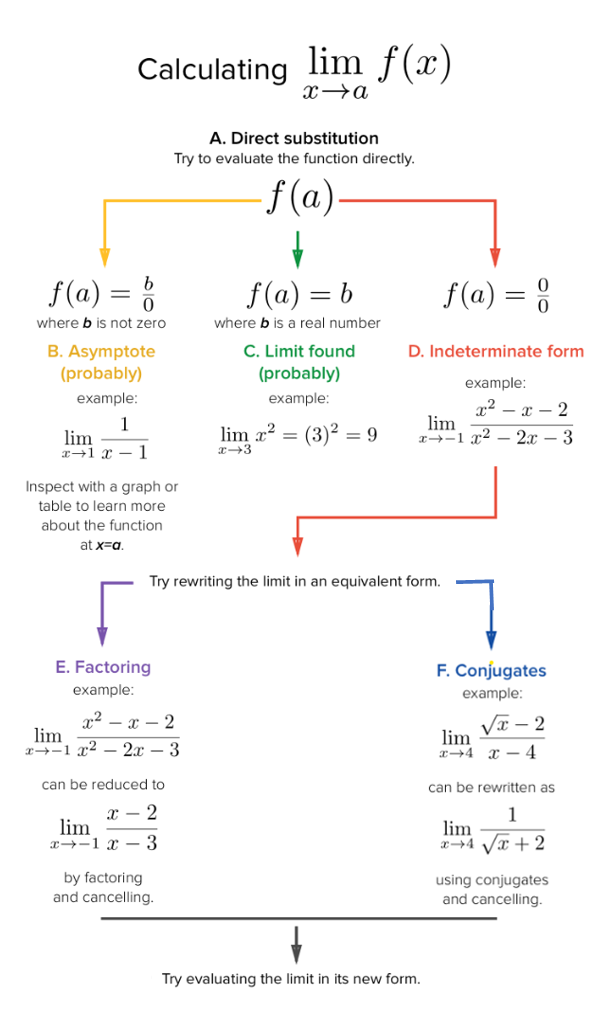
\includegraphics[width=0.75\linewidth]{img01/w01-CalculateLimit} \end{center}

\hypertarget{sum-rule-1}{%
\subsection{Sum Rule}\label{sum-rule-1}}

This rule states that the limit of the sum of two functions is equal to the sum of their limits:
\[
\lim_{x\to a}[f_1(x) + f_2(x) ] = \lim_{x\to a}f_1(x) + \lim_{x\to a}f_2(x).
\]

\hypertarget{constant-function-rule-1}{%
\subsection{Constant Function Rule}\label{constant-function-rule-1}}

The limit of a constant function is the constant: \[\lim_{x\to a} C = C.\]

\hypertarget{constant-multiple-rule-1}{%
\subsection{Constant Multiple Rule}\label{constant-multiple-rule-1}}

The limit of constant times a function is equal to the product of the constant and the limit of the function:

\[
\lim_{x\to a}Cf(x) = k\lim_{x\to a}f(x).
\]

\hypertarget{product-rule-1}{%
\subsection{Product Rule}\label{product-rule-1}}

This rule says that the limit of the product of two functions is the product of their limits (if they exist):

\[
\lim_{x\to a}[f_1(x)f_2(x)] = \lim_{x\to a}f_1(x)\lim_{x\to a}f(x)
\]

\hypertarget{quotient-rule-1}{%
\subsection{Quotient Rule}\label{quotient-rule-1}}

The limit of the quotient of two functions is the quotient of their limits, provided that the limit in the denominator function is not zero:
\[
\lim_{x\to a}\frac{f(x)}{g(x)} = \frac{\lim_{x\to a}f(x)}{\lim_{x\to a}g(x)}.
\]

\hypertarget{power-rule-1}{%
\subsection{Power Rule}\label{power-rule-1}}

For any real number \(p\),
\[
\lim_{x\to a}[f(x)]^p = [\lim_{x\to a}f(x)]^p.
\]
In particular,

\[
\lim_{x\to a}\sqrt[p]{f(x)} = \sqrt[p]{\lim_{x\to a}f(x)}.
\]

\hypertarget{algebraic-calculation-of-limits-by-examples-1}{%
\section{Algebraic Calculation of Limits by Examples}\label{algebraic-calculation-of-limits-by-examples-1}}

\textbf{Example 1}: Compute the value of the following limit
\[
\lim_{x\to -2}(3x^2 + 5x -9).
\]

\textbf{Solution}:

\[
\lim_{x\to -2}(3x^2 + 5x -9) = 3[\lim_{x\to -2} x]^2 + 5\lim_{x\to -2}x - \lim_{x\to -2}9 = 3\times (-2)^2 + 5(-2) - 9 = -7.
\]

\textbf{Example 2}: Evaluate the following limit.

\[
\lim_{x\to 1}\frac{6-3x+10x^2}{-2x^4+7x^3+1}.
\]
\textbf{Solution}: Using properties of limit, we have

\[
\lim_{x\to 1}\frac{6-3x+10x^2}{-2x^4+7x^3+1}=\frac{\lim_{x\to 1}[6-3x+10x^2]}{\lim_{x\to 1}[-2x^4+7x^3+1]}=\frac{6-3(1)+10(1)^2}{-2(1)^4+7(1)^3+1}=\frac{13}{6}.
\]

\textbf{Example 3} Find the limit

\[
\lim_{x\to 9}\frac{4x^2}{1+\sqrt{x}}.
\]

\textbf{Solution}: Using the properties of limits (the sum rule, the power rule, and the quotient rule), we get \[
\lim_{x\to 9}\frac{4x^2}{1+\sqrt{x}}=\frac{\lim_{x\to 9}(4x^2)}{\lim_{x\to 9}(1+\sqrt{x})} = \frac{4\lim_{x\to 9}(x^2)}{(\lim_{x\to 9}1+\lim_{x\to 9}\sqrt{x})} = \frac{4\times 9^2}{(1+\sqrt{9})} = 81.
\]

\textbf{Example 4}: Suppose that \(\lim_{x\to 1}f(x) = 2\) and \(\lim_{x \to 1}g(x) = 3\). Calculate the limit

\[
 \frac{g(x) - 3f(x)}{f^2(x) + g(x)}
 \]

\textbf{Solution}: Using the properties of limit, we have
\[
\lim_{x\to 1} \frac{g(x) - 3f(x)}{f^2(x) + g(x)} =  \frac{\lim_{x\to 1}[g(x) - 3f(x)]}{\lim_{x\to 1}[f^2(x) + g(x)]} = \frac{\lim_{x\to 1}g(x) - 3\lim_{x\to 1}f(x)}{[\lim_{x\to 1}f(x)]^2 + \lim_{x\to 1}g(x)} = -\frac{3}{7}.
\]

\hypertarget{average-rate-of-change.-1}{%
\section{Average Rate of Change.}\label{average-rate-of-change.-1}}

Often times we are not just interested in a function \(f(x)\) itself but also in how \(f(x)\) changes. To be specific, we may be interested in how much the function changed per unit, on average, over an interval.

\hypertarget{average-rate-of-change-of-a-function-over-an-interval-1}{%
\section{Average rate of change of a function over an interval}\label{average-rate-of-change-of-a-function-over-an-interval-1}}

\textbf{Average rate of change of a function} \(f(x)\) over an interval {[}\(a, b\){]} for \(a \ne b\) is defined to be \[
\frac{f(b)-f(a)}{b-a}
\] The geometric interpretation of the average rate of change is the slope of the secant line defined based on the interval.

\begin{center}\includegraphics[width=0.45\linewidth]{img01/w01note16-SecantLineSlope} \end{center}

\textbf{Example}: According to Google Maps, it's about 33 miles from WCU to the Independent Hall in Philadelphia. If Kevin made this trip in 45 minutes, what was his average rate of travel during the trip?

\begin{center}\includegraphics[width=0.65\linewidth]{img01/w01note17-RateChangeDistance} \end{center}

\textbf{Solution}: Let \(t\) be the driving time and \(f(t)\) the driving distance (that is a function of time \(t\)). We set \(t=0\) at the starting point, i.e., \(f(0)=0\). Since it takes 0.75 hours to drive to the destination, this means \(f(0.75) = 33\). Now based on the definition of \textbf{the rate of change of the distance function} \(f(t)\) on interval \([0, 0.75]\), we have \[
V = \frac{f(0.75) - f(0)}{0.75-0} = \frac{33-0}{0.75-0} = \frac{33}{0.75} = 44.
\] The rate of change is 44 miles per hour.

\textbf{Example}: In 1998, Linda purchased a house for \$144,000. In 2009, the house was worth \$245,000. Find the average annual rate of change in dollars per year in the value of the house. Round your answer to the nearest dollar.

\textbf{Solution}: Since house prices (\(P\)) change over time (\(t\)), therefore, house price is a function of time \(P(t)\). The objective is to find the annual rate of change of the house price. It is natural to use the year as the time variable \(t\) and set \(f(1998) = 144000\) and \(f(2009) = 245000\). Then the annual rate of change is \[
\frac{f(2009) - f(1998)}{2009 - 1998} = \frac{245000-144000}{2009-1998} \approx 9182.
\]

The annual rate of change is approximately equal to \$9182.

\hypertarget{difference-quotient-1}{%
\subsection{Difference quotient}\label{difference-quotient-1}}

The difference quotient of a (single variable) function is usually the name for the following expression

\[
\frac{f(x+h)-f(x)}{h}.
\]

This is a variation of the formula of the rate of change

\[
\frac{f(b)-f(a)}{b -a}
\]

where \(a = x\) and \(h = b -a\). We usually assume that \(h\) is close to zero. Without loss of generality, \(h\) is usually assumed to be a small positive number close to zero.

The notation of the difference quotient is easy to use to describe the derivative of a function.

\textbf{Example}: Find the difference quotient of \(f(x) = x^2 + 4x -6\).

\textbf{Solution}: Using the definition of the difference of quotient, we have
\[
\frac{f(x+h)-f(x)}{h} = \frac{[(x+h)^2 + 4(x+h) -6]-[x^2+4x-6]}{h}=\frac{2hx+h^2+4h}{h}=2x+h+4.
\]

\textbf{Example}: Find the difference quotient of \(f(x) = \sqrt{x}\).

\textbf{Solution}: Using the formula of the difference quotient, we have
\[
\frac{\sqrt{x+h}-\sqrt{x}}{h} = \frac{(\sqrt{x+h}-\sqrt{x})(\sqrt{x+h}+\sqrt{x})}{h(\sqrt{x+h}-\sqrt{x})} = \frac{(x+h)-x}{{h(\sqrt{x+h}+\sqrt{x})}} = \frac{1}{\sqrt{x+h}+\sqrt{x}}.
\]

\textbf{Example}: Let \(D\) be on the elasticity of demand that is generally defined in the following
\[
D = \frac{tC}{P + t}
\]

where \(P,t, C\) are respectively price, tax, and constant. We are interested in the effect of the tax change on demand by looking at the difference quotient.

\textbf{Solution}: By the definition of \textbf{difference quotient}, we have
\[
\frac{D(t+h) - D(t)}{h} = \frac{\frac{(t+h)C}{P+(t+h)}-\frac{tC}{P+t}}{h} = \frac{(t+h)C}{h(P+t+h)}-\frac{tC}{h(P+t)}
\]

\hypertarget{rate-of-change-and-derivative-of-functions}{%
\chapter{Rate of Change and Derivative of Functions}\label{rate-of-change-and-derivative-of-functions}}

This note focuses on the rationale of the definition of derivative of a given function. Since the concept of limit is the step-stone to the definition of the derivative, we will repeat the the definitions, properties, and calculations of limits before introducing the concepts of derivative and its geometry.

\hypertarget{review-concepts-of-limits}{%
\section{Review: Concepts of Limits}\label{review-concepts-of-limits}}

We have described how to find the limit of a function at a given point graphically. Next we introduce how to find limit algebraically. The basic method is \textbf{substitution}. The following \textbf{\color{red}updated chart} outlines the workflow in calculating the limit of a given function at a given value of the independent variable.

\begin{center}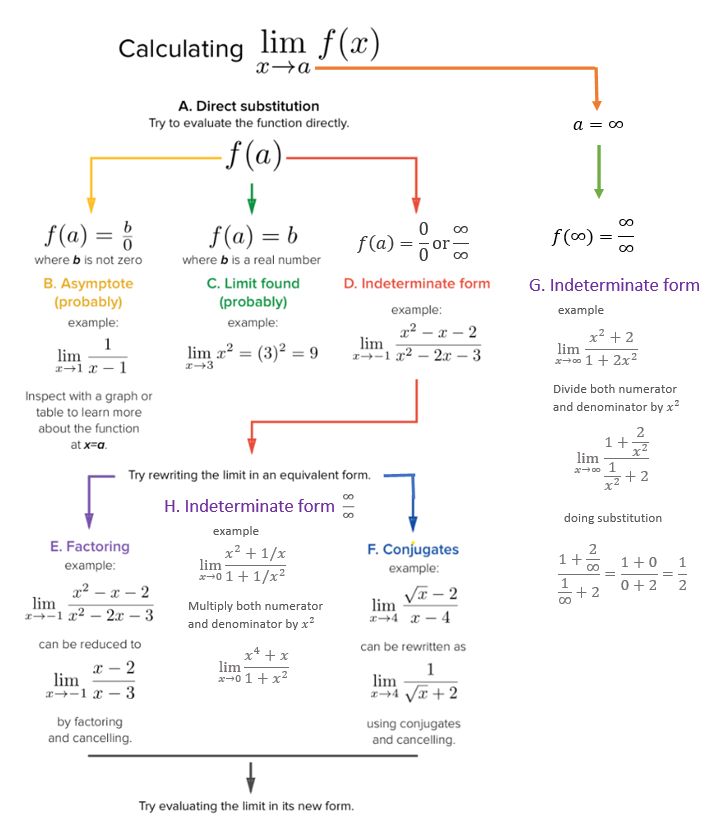
\includegraphics[width=0.85\linewidth]{img02/w01-CalculateLimit} \end{center}

\hfill\break

Recall that when left and right limits are not equal or at least one of one-sided limits is equal to \(\infty\) or \(-\infty\), we call the limit does not exist. As an exercise, find \(x\) values at which the limit does not exist.

\begin{center}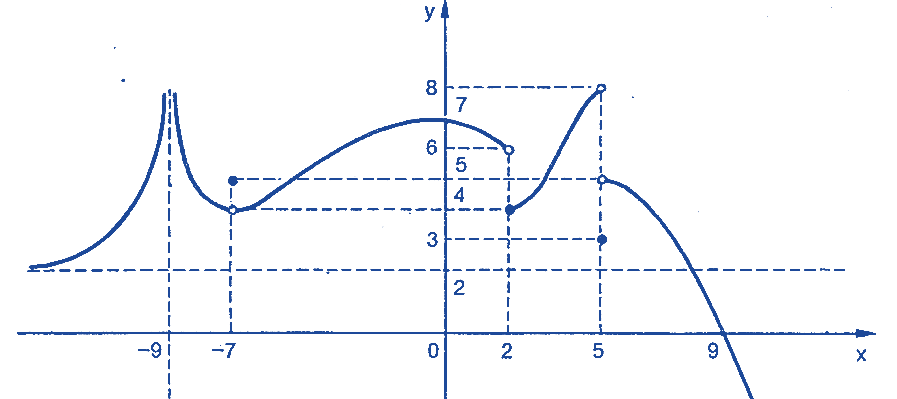
\includegraphics[width=0.75\linewidth]{img02/w02note-limitDoesNotExist} \end{center}

\textbf{Answer}: \(x = -0, 2, 5\)

\hfill\break

\hypertarget{properties-of-limits-1}{%
\section{Properties of Limits}\label{properties-of-limits-1}}

\hypertarget{sum-rule-2}{%
\subsection{Sum Rule}\label{sum-rule-2}}

This rule states that the limit of the sum of two functions is equal to the sum of their limits:
\[
\lim_{x\to a}[f_1(x) + f_2(x) ] = \lim_{x\to a}f_1(x) + \lim_{x\to a}f_2(x).
\]

\hypertarget{constant-function-rule-2}{%
\subsection{Constant Function Rule}\label{constant-function-rule-2}}

The limit of a constant function is the constant: \[\lim_{x\to a} C = C.\]

\hypertarget{constant-multiple-rule-2}{%
\subsection{Constant Multiple Rule}\label{constant-multiple-rule-2}}

The limit of constant times a function is equal to the product of the constant and the limit of the function:
\[
\lim_{x\to a}Cf(x) = k\lim_{x\to a}f(x).
\]

\hypertarget{product-rule-2}{%
\subsection{Product Rule}\label{product-rule-2}}

This rule says that the limit of the product of two functions is the product of their limits (if they exist):
\[
\lim_{x\to a}[f_1(x)f_2(x)] = \lim_{x\to a}f_1(x)\lim_{x\to a}f(x)
\]

\hypertarget{quotient-rule-2}{%
\subsection{Quotient Rule}\label{quotient-rule-2}}

The limit of the quotient of two functions is the quotient of their limits, provided that the limit in the denominator function is not zero:
\[
\lim_{x\to a}\frac{f(x)}{g(x)} = \frac{\lim_{x\to a}f(x)}{\lim_{x\to a}g(x)}.
\]

\hypertarget{power-rule-2}{%
\subsection{Power Rule}\label{power-rule-2}}

For any real number \(p\),
\[
\lim_{x\to a}[f(x)]^p = [\lim_{x\to a}f(x)]^p.
\]
In particular,

\[
\lim_{x\to a}\sqrt[p]{f(x)} = \sqrt[p]{\lim_{x\to a}f(x)}.
\]

\hypertarget{algebraic-calculation-of-limits-by-examples-2}{%
\subsection{Algebraic Calculation of Limits by Examples}\label{algebraic-calculation-of-limits-by-examples-2}}

\textbf{Example 1}: Compute the value of the following limit
\[
\lim_{x\to -2}(3x^2 + 5x -9).
\]

\textbf{Solution}:

\[
\lim_{x\to -2}(3x^2 + 5x -9) = 3[\lim_{x\to -2} x]^2 + 5\lim_{x\to -2}x - \lim_{x\to -2}9 = 3\times (-2)^2 + 5(-2) - 9 = -7.
\]

\textbf{Example 2}: Evaluate the following limit.

\[
\lim_{x\to 1}\frac{6-3x+10x^2}{-2x^4+7x^3+1}.
\]
\textbf{Solution}: Using properties of limit, we have

\[
\lim_{x\to 1}\frac{6-3x+10x^2}{-2x^4+7x^3+1}=\frac{\lim_{x\to 1}[6-3x+10x^2]}{\lim_{x\to 1}[-2x^4+7x^3+1]}=\frac{6-3(1)+10(1)^2}{-2(1)^4+7(1)^3+1}=\frac{13}{6}.
\]

\textbf{Example 3} Find the limit

\[
\lim_{x\to 9}\frac{4x^2}{1+\sqrt{x}}.
\]

\textbf{Solution}: Using the properties of limits (the sum rule, the power rule, and the quotient rule), we get \[
\lim_{x\to 9}\frac{4x^2}{1+\sqrt{x}}=\frac{\lim_{x\to 9}(4x^2)}{\lim_{x\to 9}(1+\sqrt{x})} = \frac{4\lim_{x\to 9}(x^2)}{(\lim_{x\to 9}1+\lim_{x\to 9}\sqrt{x})} = \frac{4\times 9^2}{(1+\sqrt{9})} = 81.
\]

\textbf{Example 4}: Suppose that \(\lim_{x\to 1}f(x) = 2\) and \(\lim_{x \to 1}g(x) = 3\). Calculate the limit
\[
 \frac{g(x) - 3f(x)}{f^2(x) + g(x)}
 \]

\textbf{Solution}: Using the properties of limit, we have
\[
\lim_{x\to 1} \frac{g(x) - 3f(x)}{f^2(x) + g(x)} =  \frac{\lim_{x\to 1}[g(x) - 3f(x)]}{\lim_{x\to 1}[f^2(x) + g(x)]} = \frac{\lim_{x\to 1}g(x) - 3\lim_{x\to 1}f(x)}{[\lim_{x\to 1}f(x)]^2 + \lim_{x\to 1}g(x)} = -\frac{3}{7}.
\]

\hfill\break

\hypertarget{average-rate-of-change.-2}{%
\section{Average Rate of Change.}\label{average-rate-of-change.-2}}

Often times we are not just interested in a function \(f(x)\) itself but also in how \(f(x)\) changes. To be specific, we may be interested in how much the function changed per unit, on average, over an interval.

\hypertarget{average-rate-of-change-of-a-function-over-an-interval-2}{%
\subsection{Average rate of change of a function over an interval}\label{average-rate-of-change-of-a-function-over-an-interval-2}}

\textbf{Average rate of change of a function} \(f(x)\) over an interval {[}\(a, b\){]} for \(a \ne b\) is defined to be
\[
\frac{f(b)-f(a)}{b-a}
\]
The geometric interpretation of the average rate of change is the slope of the secant line defined based on the interval.

\begin{center}\includegraphics[width=0.45\linewidth]{img02/w01note16-SecantLineSlope} \end{center}

\textbf{Example}: According to Google Maps, it's about 33 miles from WCU to the Independent Hall in Philadelphia. If Kevin made this trip in 45 minutes, what was his average rate of travel during the trip?

\begin{center}\includegraphics[width=0.65\linewidth]{img02/w01note17-RateChangeDistance} \end{center}

\textbf{Solution}: Let \(t\) be the driving time and \(f(t)\) the driving distance (that is a function of time \(t\)). We set \(t=0\) at the starting point, i.e., \(f(0)=0\). Since it takes 0.75 hours to drive to the destination, this means \(f(0.75) = 33\). Now based on the definition of \textbf{the rate of change of the distance function} \(f(t)\) on interval \([0, 0.75]\), we have \[
V = \frac{f(0.75) - f(0)}{0.75-0} = \frac{33-0}{0.75-0} = \frac{33}{0.75} = 44.
\] The rate of change is 44 miles per hour.

\textbf{Example}: In 1998, Linda purchased a house for \$144,000. In 2009, the house was worth \$245,000. Find the average annual rate of change in dollars per year in the value of the house. Round your answer to the nearest dollar.

\textbf{Solution}: Since house prices (\(P\)) change over time (\(t\)), therefore, house price is a function of time \(P(t)\). The objective is to find the annual rate of change of the house price. It is natural to use the year as the time variable \(t\) and set \(f(1998) = 144000\) and \(f(2009) = 245000\). Then the annual rate of change is

\[
\frac{f(2009) - f(1998)}{2009 - 1998} = \frac{245000-144000}{2009-1998} \approx 9182.
\]

The annual rate of change is approximately equal to \$9182.

\hfill\break

\hypertarget{definition-of-derivative}{%
\section{Definition of Derivative}\label{definition-of-derivative}}

We know that the average of change of a function at \(P(x_1, y_1)\) and \(Q(x_2, y_2)\) represents the slope of secant line of the line passing through points \(P\) and \(Q\). This section discuss the concepts of derivative. Before we introduce the definition of derivative, we need a few related concepts.

When \(Q(x_2, y_2)\) moves to \(P(x_1, x_2)\), the secant line eventually becomes the tangent line at \(P(x_1, y_1)\). This limiting process is demonstrated in the following animated graph.

\hfill\break

\url{https://github.com/pengdsci/MAT143/raw/main/w02/img/w02-SecantTangentSlopes.gif}

\hypertarget{difference-quotient-2}{%
\subsection{Difference quotient}\label{difference-quotient-2}}

The difference quotient of a (single variable) function is usually the name for the following expression

\[
\frac{f(x+h)-f(x)}{h}.
\]

This is a variation of the formula of the rate of change

Recall that the average rate of change of a function at two points \(P(a,f(a))\) and \(Q(b, f(b))\) is given by

\[
\frac{f(b)-f(a)}{b -a}.
\]

If we denote \(x = a\) and \(h = b-a\), the coordinates of \(P\) and \(Q\) can be re-expressed as \(P(x, f(x))\) and \(Q(a+h, f(a+b))\). The corresponding rate of change can be re-written as

\[
\frac{f(x+h)-f(x)}{(x+h) - x} = \frac{f(x+h)-f(x)}{h}.
\]

The above notation is called the \textbf{difference quotient}. In general, \(h\) is distance between points \(P\) and \(Q\). \(h \to 0\) implies that \(Q\) moves to \(P\).

\begin{center}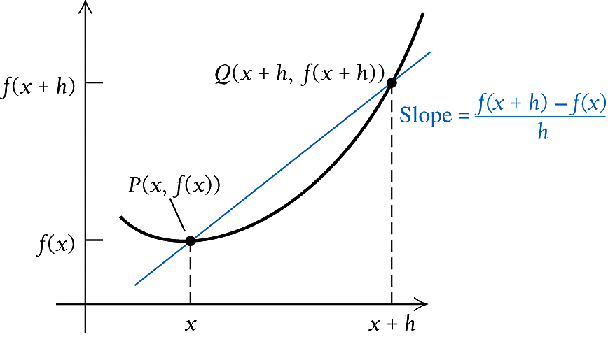
\includegraphics[width=0.65\linewidth]{img02/w02note-DifferenceQuotient} \end{center}

With the above notation, we can find the \textbf{difference quotient} for a function with explicit expression. Next are few examples.

\hfill\break

\textbf{Example 1}: Find the difference quotient of \(f(x) = x^2 + 4x -6\).

\textbf{Solution}: Using the definition of the difference of quotient, we have
\[
\frac{f(x+h)-f(x)}{h} = \frac{[(x+h)^2 + 4(x+h) -6]-[x^2+4x-6]}{h}=\frac{2hx+h^2+4h}{h}=2x+h+4.
\]

\hfill\break

\textbf{Example 2}: Find the difference quotient of \(f(x) = \sqrt{x}\).

\textbf{Solution}: Using the formula of the difference quotient, we have
\[
\frac{\sqrt{x+h}-\sqrt{x}}{h} = \frac{(\sqrt{x+h}-\sqrt{x})(\sqrt{x+h}+\sqrt{x})}{h(\sqrt{x+h}-\sqrt{x})} = \frac{(x+h)-x}{{h(\sqrt{x+h}+\sqrt{x})}} = \frac{1}{\sqrt{x+h}+\sqrt{x}}.
\]

\hfill\break

\hypertarget{instantaneous-rate-of-change-derivative}{%
\subsection{Instantaneous Rate of Change: Derivative}\label{instantaneous-rate-of-change-derivative}}

The slope of the tangent line the passes \(P(c, f(c))\) and \(Q(c+h, f(c+h))\) is given by
\[
\frac{f(c+h) - f(c)}{h}.
\]

The limit of the above \textbf{difference quotient} when \(t \to 0\) is the slope of the tangent line at \(P\).
\[
\text{Slope of the tangent line at P} = \lim_{h \to 0} \frac{f(c+h) - f(c)}{h}
\]

\hfill\break

\url{https://github.com/pengdsci/MAT143/raw/main/w02/img/w02-derivative.gif}

\textbf{Definition}: The derivative of \(f(x)\) at \(x = c\) is defined to be the slope of the tangent line at \(P(c, f(c))\). We use notation \(f^\prime(c)\) is used to denote the derivative of \(f(x)\) at \(x = c\).

\textbf{Definition}: If the derivative of \(f(x)\) exists at \(x = c\), we also call that \(f(x)\) is differential at \(x = c\).

\hfill\break

\hypertarget{finding-derivatives}{%
\subsection{Finding Derivatives}\label{finding-derivatives}}

Since the derivative of a function at a given point \(x = c\) is the limit of the \textbf{difference quotient} of the function at \(x = c\). This means, to calculate the derivative of a function, we need to find the \textbf{difference quotient} first, then take the limit at \(h = 0\).

\textbf{Example 3}: find the derivative of \(f(x) = 5\).

\textbf{Solution}: The \textbf{difference quotient} of \(f(x) = 5\) is
\[
\frac{f(x+h) - f(x)}{h} = \frac{(5) - 5}{h} = \frac{5-5}{h} = 0.
\]
Therefore,
\[
f^\prime(x) = (5)^\prime = 0.
\]

\hfill\break

\textbf{Example 4}: find the derive of \(f(x) = x^2\).

\textbf{Solution}. We first find the \textbf{difference quotient}.

\[
\frac{f(x+h)-f(x)}{h} = \frac{(x+h)^2-x^2}{h} = \frac{(x^2+2hx+h^2)-x^2}{h} = \frac{2hx+h^2}{h} =2x+h 
\]
By definition,
\[
f^\prime(x) = \lim_{h \to 0} (2x +h) = 2x + \lim_{h \to 0}(h) = 2x.
\]

\hfill\break

\textbf{Example 5}: Find the derivative of \(f(x) = \sqrt{x}\).

\textbf{Solution}: The \textbf{Difference quotient} of \(f(x) = \sqrt{x}\) is given by

\[
\frac{f(x+h) - f(x)}{h} = \frac{\sqrt{x+h})-\sqrt{x}}{h} = \frac{(\sqrt{x+h}-\sqrt{x})(\sqrt{x+h}+\sqrt{x})}{h(\sqrt{x+h}+\sqrt{x})} = \frac{1}{\sqrt{x+h}+\sqrt{x}}
\]
Therefore,
\[
f^\prime(x) = \lim_{h \to 0}\frac{1}{\sqrt{x+h}+\sqrt{x}} = \frac{1}{2\sqrt{x}}
\]

\hfill\break

\hypertarget{basic-rules-of-derivatives---part-i.}{%
\section{Basic Rules of Derivatives - Part I.}\label{basic-rules-of-derivatives---part-i.}}

For convenience, we first introduce some basic rules of derivative before calculating the derivative of functions with more complex forms.

\hypertarget{power-rule-3}{%
\subsection{Power Rule}\label{power-rule-3}}

Recall that the Power function is defined by

\[
f(x) = x^a
\]

Where the power \(a\) is an arbitrary real number. The derivative of the function is defined to be

\begin{center}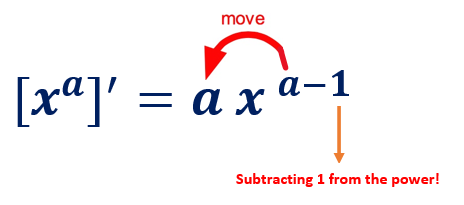
\includegraphics[width=0.45\linewidth]{img02/w02note-PowerRule} \end{center}

Next, we use the above power rule to do a few examples.Some of the functions are not in the standard form of the power function, but we can re-express it into the standard form. For example, \(f(x) = 1/\sqrt{x} = x^{1/2}\), \(f(x) = 1/x = x^{-1}\), etc.

\textbf{Example 6}: Find the derive of \(f(x) = 1/\sqrt[5]{x^2}\).

\textbf{Solution}: We first re-express the given function in the the standard form of power function and then take the derivative using the power rule.

\[
f^\prime(x) = (1/\sqrt[5]{x^2})^\prime = \left( x^{-2/5}\right)^\prime = (-2/5)x^{-2/5 - 1} = -\frac{2}{5}x^{-7/5}.
\]

\hypertarget{additive-rule}{%
\subsection{Additive Rule}\label{additive-rule}}

The additive rule deals with the derivative of the sum of functions. To be more specific,

\textbf{Additive Rule}: Let \(f(x)\) and \(g(x)\) be two \emph{differentiable} functions (that have derivatives (i.e., the derivative of both functions exist). Then
\[
[f(x) + g(x)]^\prime = f^\prime(x) + g^\prime(x).
\]

Next, we use the additive rule to find the derivative of function with more complex forms.

\textbf{Example 7}: Find the derivative of \(f(x) = 5 + x^3\).

\textbf{Solution}: Using the additive and power rule, we have
\[
f^\prime(x) = (5 + x^3)^\prime = (5)^\prime + (x^3)^\prime = 0 + 3x^{3-1} = 3x^2.
\]

\textbf{Example 8}: Find the derivative of \(f(x) = x + \sqrt{x}\)

\textbf{Solution}: We first express each term into power function then take derivative

\[
f^\prime(x) = (x + \sqrt{x})^\prime = (x^1)^\prime + (x^{1/2})^\prime = 1x^{1-1} + (1/2)x^{1/2-1} = 1 + \frac{1}{2\sqrt{x}}.
\]

\hypertarget{summary-and-more-examples}{%
\subsection{Summary and More Examples}\label{summary-and-more-examples}}

In this week, we defined the derive of a function \(y = f(x)\), denoted by \(y^\prime = f^\prime(x)\), to be instantaneous rate of change
\[
f^\prime(x) = \lim_{h \to 0}\frac{f(x+h)-f(x)}{h}
\]

The following basic rules were also introduced to make the calculation of derivative easier.

\begin{enumerate}
\def\labelenumi{\arabic{enumi}.}
\item
  \(f(x) = c\), then \(f^\prime(x) = (c)^\prime = 0\).
\item
  \(f(x) = x\), then \(f^\prime(x) = (x)^\prime = 1\).
\item
  \(f(x) = x^a\), then \(f^\prime(x) = (x^a)^\prime = ax^{a-1}\). for any real number \(a\).
\end{enumerate}

Properties:

\begin{enumerate}
\def\labelenumi{\arabic{enumi}.}
\item
  \([bf(x)]^\prime = b[f(x)]^\prime\)
\item
  \([f(x) + g(x)]^\prime = [f(x)]^\prime + [g(x)]^\prime\)
\end{enumerate}

\hfill\break

\textbf{Example 9}. (taken from the textbook)

\begin{center}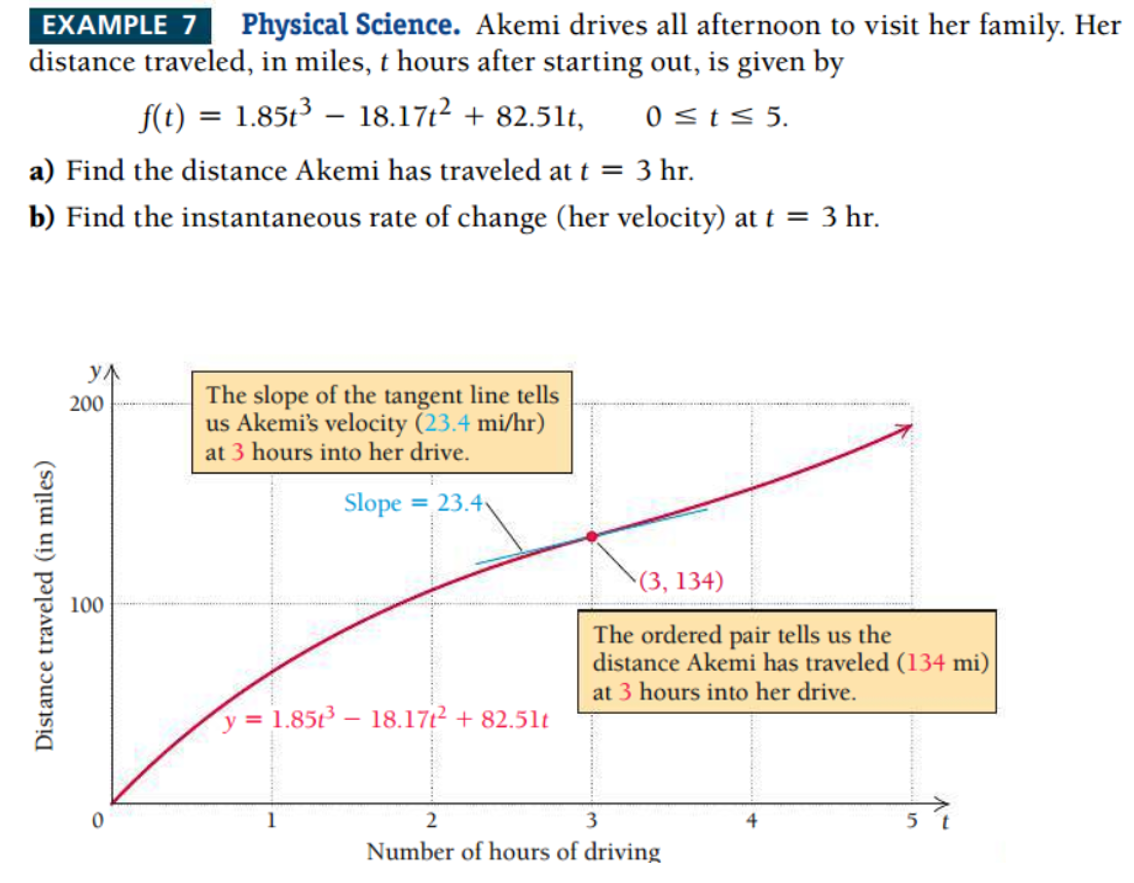
\includegraphics[width=0.75\linewidth]{img02/w02-example9} \end{center}

\hfill\break

\textbf{Example 10} (taken from the textbook)

\begin{center}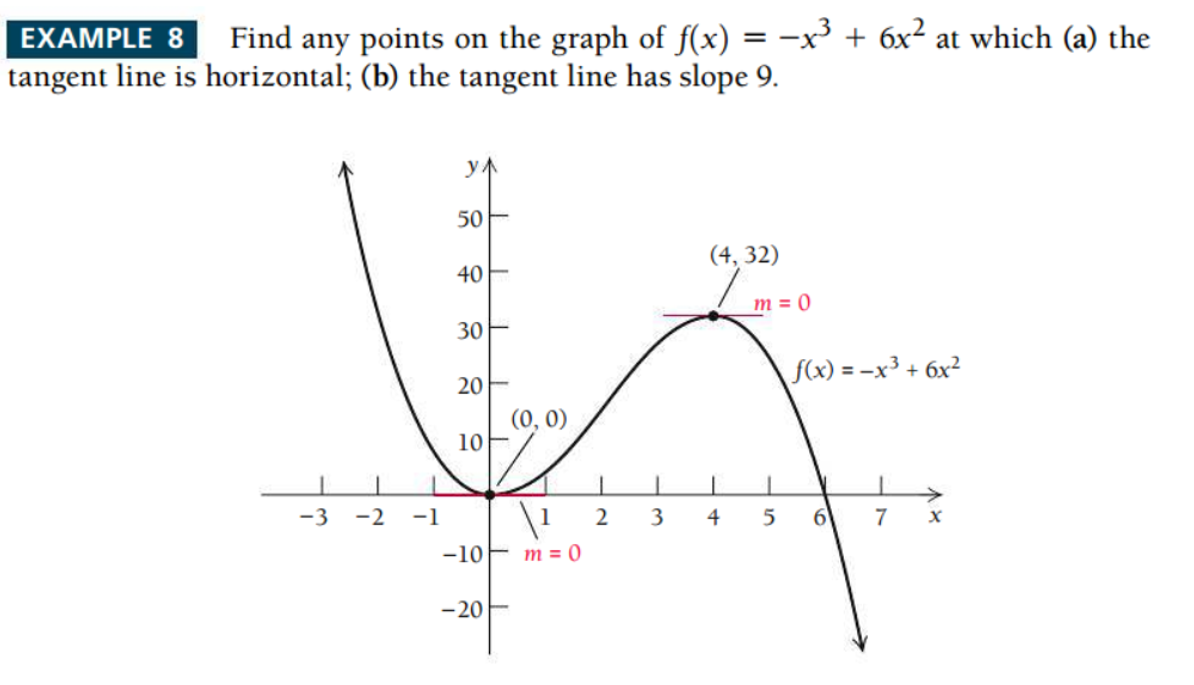
\includegraphics[width=0.75\linewidth]{img02/w02-example10-1} \end{center}

\begin{center}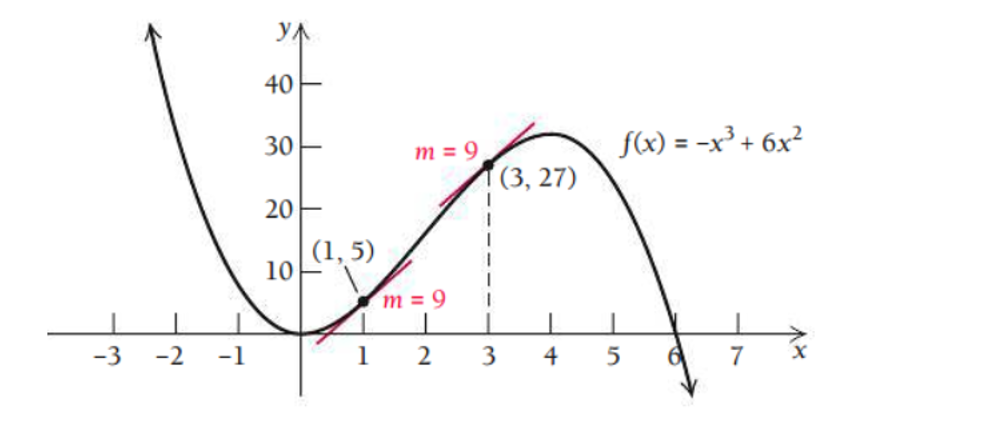
\includegraphics[width=0.75\linewidth]{img02/w02-example10-2} \end{center}

\hypertarget{rules-of-derivative}{%
\chapter{Rules of Derivative}\label{rules-of-derivative}}

This note focuses on the basic rules of derivative.

\hypertarget{review-of-derivative}{%
\section{Review of Derivative}\label{review-of-derivative}}

We defined the derivative of a function \(y = f(x)\), denoted by \(y^\prime = f^\prime(x)\), to be instantaneous rate of change
\[
f^\prime(x) = \lim_{h \to 0}\frac{f(x+h)-f(x)}{h}
\]

The following basic rules were also introduced to calculate derivatives easier.

\begin{enumerate}
\def\labelenumi{\arabic{enumi}.}
\item
  \(f(x) = c\), then \(f^\prime(x) = (c)^\prime = 0\).
\item
  \(f(x) = x\), then \(f^\prime(x) = (x)^\prime = 1\).
\item
  \(f(x) = x^a\), then \(f^\prime(x) = (x^a)^\prime = ax^{a-1}\). for any real number \(a\).
\end{enumerate}

\begin{center}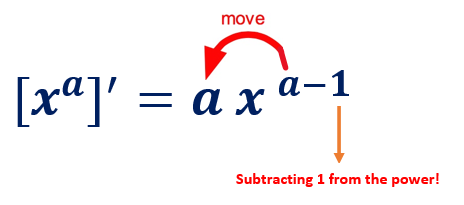
\includegraphics[width=0.6\linewidth]{img03/w03note-PowerRule} \end{center}

Properties:

\begin{enumerate}
\def\labelenumi{\arabic{enumi}.}
\item
  \([bf(x)]^\prime = b[f(x)]^\prime\)
\item
  \([f(x) + g(x)]^\prime = [f(x)]^\prime + [g(x)]^\prime\)
\end{enumerate}

We will continue to introduce more rules and properties of derivatives this week.

\hfill\break

\hypertarget{leibniz-notation}{%
\section{Leibniz Notation}\label{leibniz-notation}}

In calculus, \textbf{Leibniz's notation} uses the symbols \(dx\) and \(dy\) to represent infinitely small (or infinitesimal) increments of \(x\) and \(y\), respectively, just as \(\Delta x\) and \(\Delta y\) represent finite increments of \(x\) and \(y\), respectively.

Consider \(y\) as a function of a variable \(x\), or \(y = f(x)\). If this is the case, then the derivative of \(y\) with respect to \(x\), which later came to be viewed as the limit

\[
\lim_{{\Delta x\rightarrow 0}}{\frac {\Delta y}{\Delta x}}=\lim_{{\Delta x\rightarrow 0}}{\frac  {f(x+\Delta x)-f(x)}{\Delta x}},
\]

was, according to Leibniz, the quotient of an \textbf{infinitesimal increment} of \(y\) by an \textbf{infinitesimal increment} of \(x\), or

\[
\frac{dy}{dx}=f^\prime(x),
\]

The \textbf{infinitesimal increments} are called \textbf{differentials}. From now on, we will use the following notations interchangeably.

\[
\frac{d f(x)}{dx} \text{ , } \frac{d}{dx}f(x), \text{ , and } f^\prime (x)
\]

\hfill\break

\hypertarget{multiplicative-rule}{%
\section{Multiplicative Rule}\label{multiplicative-rule}}

If a function that has a complex form can be re-expressed into a product of two relatively simple functions, then we can use the \textbf{multiplicative rule} to find the derivative.

Let \(f(x)\) and \(g(x)\) be the two differentiable functions (i.e., the derivative of both functions exists everywhere in the domain).

\[
\frac{d}{dx}[f(x)g(x)] = f^\prime(x) g(x) + f(x) g^\prime(x)
\]

\hfill\break

\url{https://github.com/pengdsci/MAT143/raw/main/w03/img/w03-product-rule-calculus-animation.gif}

\hfill\break

\textbf{Example 1}: Find the derivative of the following function.

(a). \(y = \sqrt[3]{x^2}(2x - x^2)\)

(b). \(y = (6x^3 - x)(10 - 20x)\)

\textbf{Solution} We use the multiplicative rule to calculate the above derivative.

(a). \(y^\prime = [x^{2/3}(2x - x^2)]^\prime = (x^{2/3})^\prime(2x - x^2) + x^{2/3}(2x - x^2)^\prime\)
\[
= \frac{2}{3}x^{2/3-1}(2x-x^2) + x^{2/3}(2 - 2x) =\frac{2}{3}x^{-1/3}(2x-x^2)+x^{2/3}(2 - 2x)
\]
\[
=\frac{2}{3}x^{2/3}(2-x) + 2x^{2/3}(1 - x) = 2x^{2/3}[(2-x)/3+1 - x] 
\]

\[
= 2x^{2/3}\frac{2-x+3(1-x)}{3}=\frac{2x^{2/3}(5-4x)}{3}
\]

(b). \(y^\prime = [(6x^3 - x)(10 - 20x)]^\prime = (6x^3 - x)^\prime(10 - 20x) + (6x^3 - x)(10 - 20x)^\prime\)

\(= (18x^2 - x)(10 - 20x) + (6x^3 - x)\times (-20) = -480x^3+180x^2+40x-10\)

\hfill\break

\textbf{Example 2}: (This example is taken from the textbook)

\begin{center}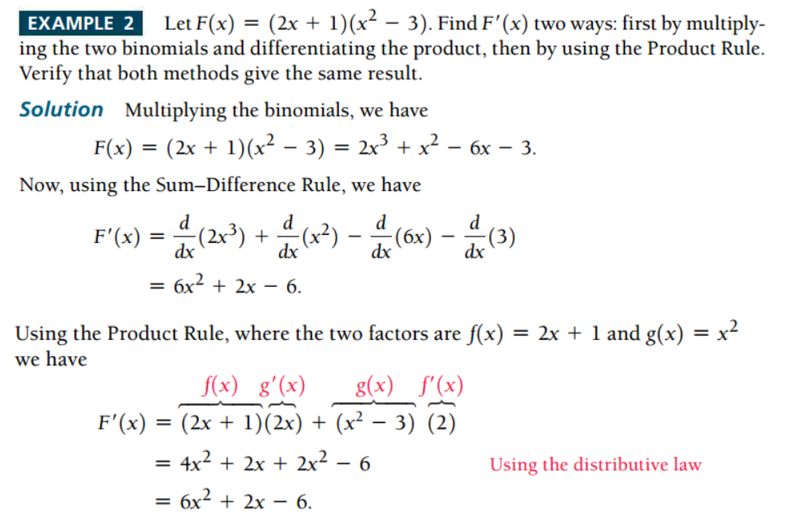
\includegraphics[width=0.8\linewidth]{img03/w03-multiplicativeExample} \end{center}

\hypertarget{quotient-rule-3}{%
\section{Quotient Rule}\label{quotient-rule-3}}

The quotient rule can be used for differentiation when taking the derivative of a function divided by another function. For example, rational functions are this type of question.

Let \(f(x)\) and \(g(x)\) be two differentiable functions. The quotient rule of the derivative is given in the following.

\[
\frac{d}{dx} \left(\frac{f(x)}{g(x)}\right)  = \frac{f^\prime(x)g(x) - f(x)g^\prime(x)}{g^2(x)}
\]

The following animated graph shows how to manipulate the terms algebraically.

\hfill\break

\url{https://github.com/pengdsci/MAT143/raw/main/w03/img/w03-quotient-rule-formula-animation.gif}

\hfill\break

\textbf{Example 3}. Find the derivative of the following functions.

(a). \(W(z) = (3z + 9)/(2 -z)\)

(b). \(h(x) = 4\sqrt{x}/(x^2 - 2)\)

\textbf{Solution}: Using the quotient rule, we have

(a). \(W^\prime(z) = [(3z+9)^\prime(2-z) - (3z+9)(2-z)^\prime]/(2-z)^2\)
\[
  = \frac{3(2-z)-(3z+9)(-1)}{(2-z)^2} = \frac{15}{(2-z)^2}
  \]

(b). \(y^\prime = \left[(4\sqrt{x})^\prime (x^2-2) -(4\sqrt{x})(x^2-2)^\prime\right]/(x^2-2)^2\)
\[
  = \frac{(2/\sqrt{x})(x^2-2)-8x\sqrt{x}}{(x^2-2)^2} = -\frac{6x\sqrt{x}+4/\sqrt{x}}{(x^2-2)^2}.
  \]

\hfill\break

\textbf{Example 4} (This example is taken from the textbook)

\begin{center}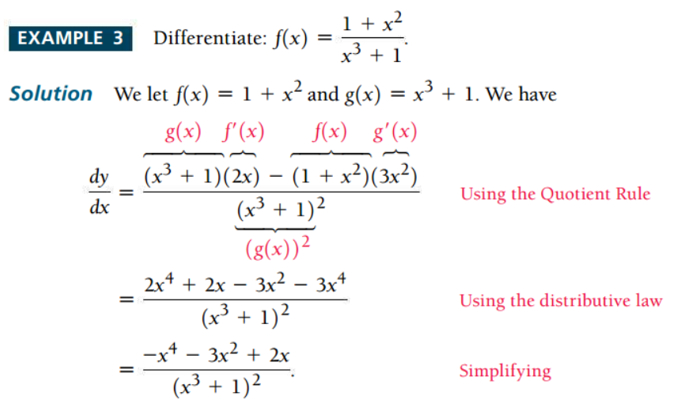
\includegraphics[width=0.7\linewidth]{img03/w03-quotientRuleExample} \end{center}

\textbf{Important Business Functions}: Cost, Revenue, and Profit-related functions and applications.

\begin{center}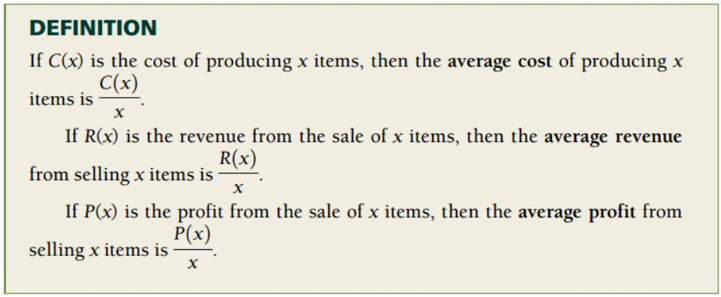
\includegraphics[width=0.7\linewidth]{img03/w03-AvgCostRevnueProfit} \end{center}

\textbf{Example 5} (This example is also taken from the textbook)

Paulsen's Greenhouse finds that the cost, in dollars, of growing x hundred geraniums is modeled by
\[
C(x) = 200 + 100 \sqrt[4]{x}
\]
If revenue from the sale of x hundred geraniums is modeled by
\[
R(x) = 120 + 90\sqrt{x}
\]\\

\begin{center}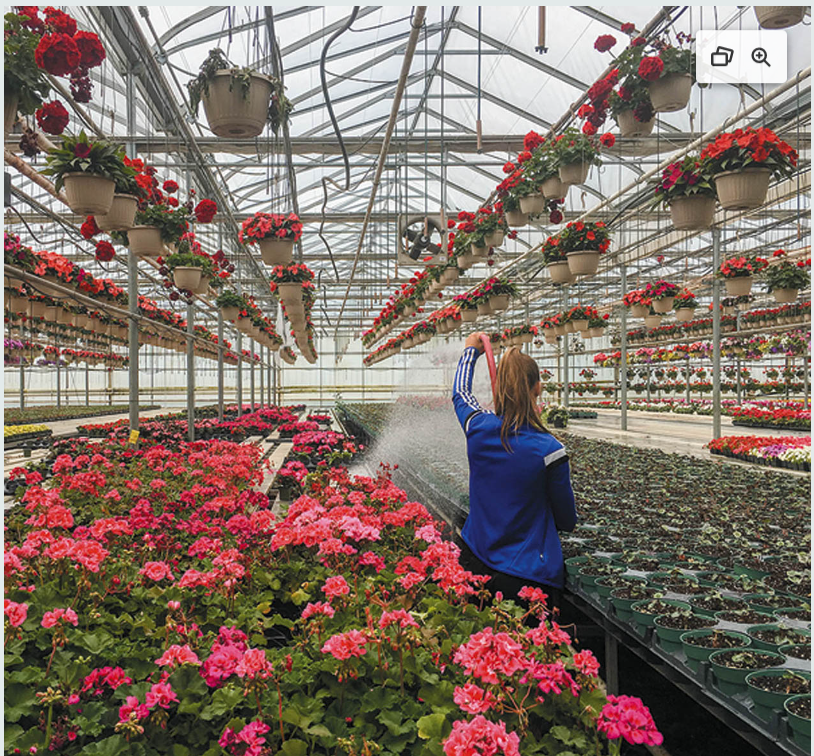
\includegraphics[width=0.55\linewidth]{img03/w03-geraniums} \end{center}

find each of the following.

\begin{enumerate}
\def\labelenumi{(\alph{enumi})}
\item
  The average cost, average revenue, and average profit when 300 geraniums are grown and sold.
\item
  The rate at which the average profit is changing when 300 geraniums are grown and sold.
\end{enumerate}

\begin{center}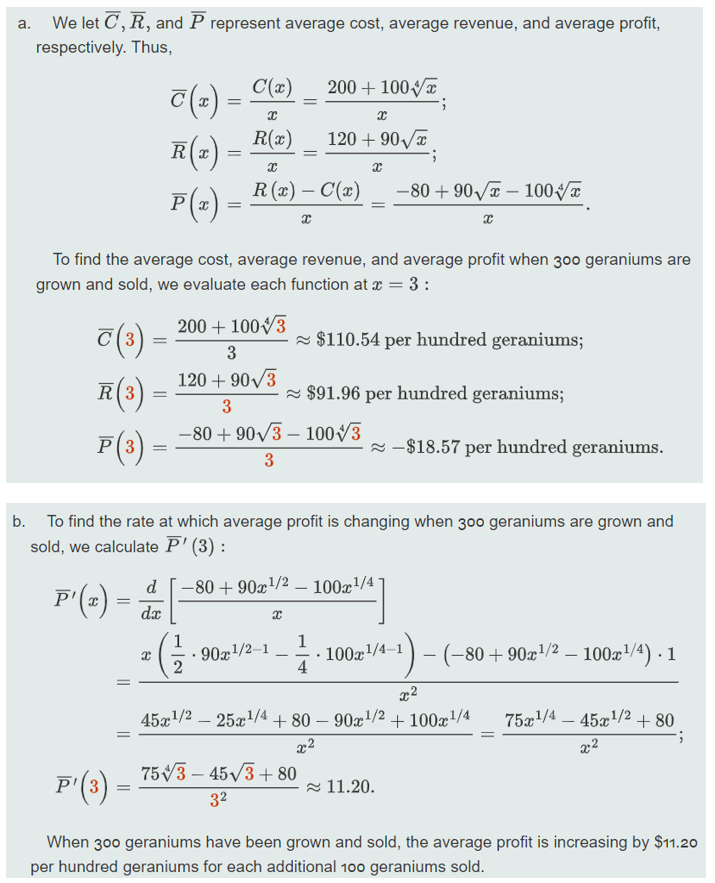
\includegraphics[width=0.75\linewidth]{img03/w03-AvgCostRevnueProfitExample} \end{center}

\hfill\break

\hypertarget{chain-rule}{%
\section{Chain Rule}\label{chain-rule}}

Before introducing the Chain Rule, we first review the definition of a composite function.

\hypertarget{composite-function}{%
\subsection{Composite Function}\label{composite-function}}

Suppose the two given functions are \(f\) and \(g\), the composition of \(f\) and \(g\), denoted by \(f\circ g\), is given by

\[
f\circ g (x) = f(g(x))  \  \  \  \text{   and   }  \ \ \ \ g\circ f (x) = g(f(x))
\]

\begin{center}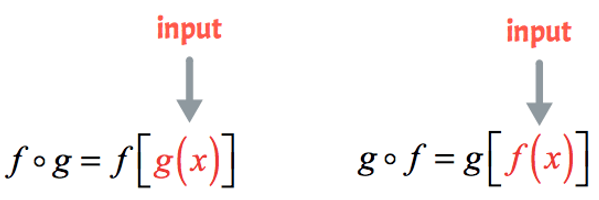
\includegraphics[width=0.55\linewidth]{img03/w03-CompositeFunction} \end{center}

\hfill\break

\textbf{Example 6} Let \(f(x) = 2x^2 - 3x -1\) and \(g(x) = -x + 5\). Find \(f\circ g\).

\begin{center}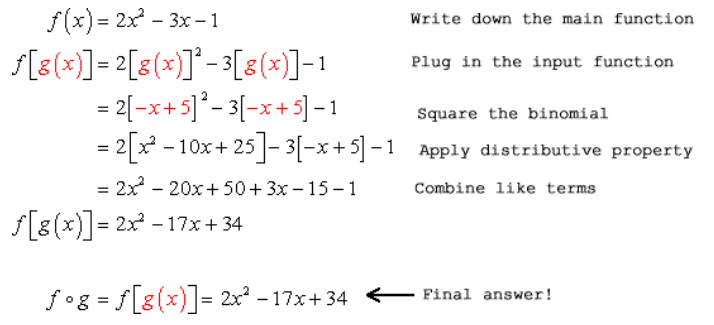
\includegraphics[width=0.75\linewidth]{img03/w03-CompositeFunEx01} \end{center}

\hfill\break

\textbf{Example 7} Let \(f(x) = 1/(x+3)\) and \(g(x) = (-3x-2)/x\). Find \(f\circ g\).

\begin{center}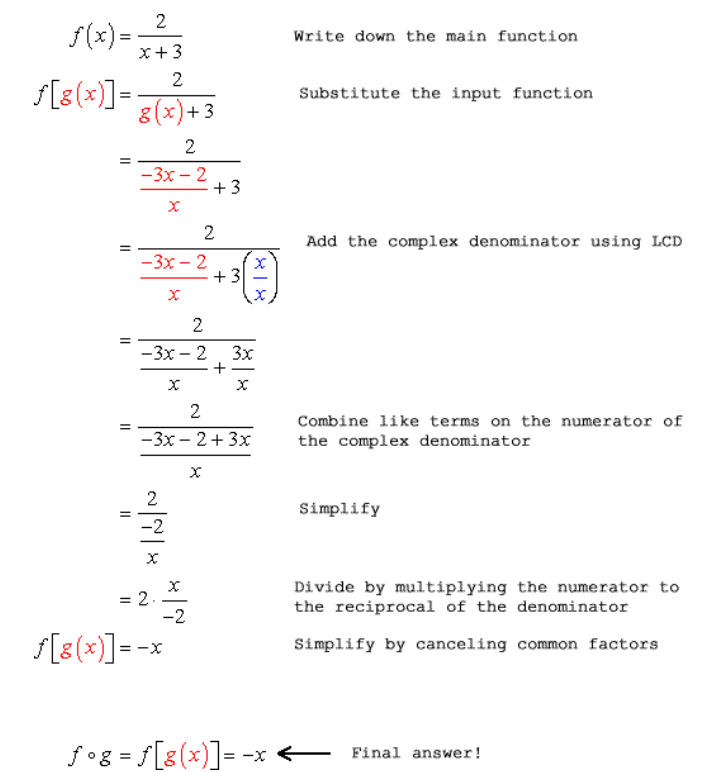
\includegraphics[width=0.8\linewidth]{img03/w03-CompositeFunEx02} \end{center}

\hfill\break

\hypertarget{chain-rule-1}{%
\subsection{Chain Rule}\label{chain-rule-1}}

The following Chain Rule is used to find the derivative of composite functions.

\[
[f(g(x))]^\prime = f^\prime(g(x)) \times g^\prime(x)
\]
\url{https://github.com/pengdsci/MAT143/raw/main/w03/img/w03-Chain-Rule-1.gif}

\textbf{Example 8} Find the derivative of the following function
\[
f(x) = \sqrt[4]{\frac{x + 3}{x - 2}}.
\]

\begin{flushleft}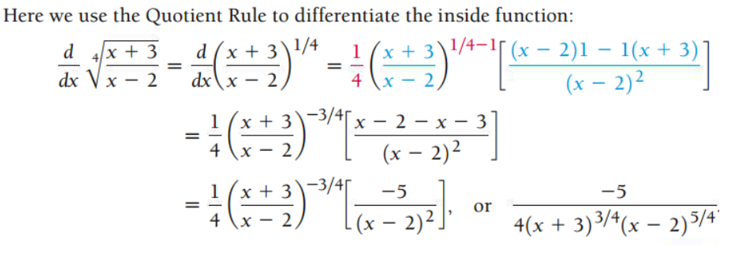
\includegraphics[width=0.7\linewidth]{img03/w03-ChainRuleEx01} \end{flushleft}

\textbf{Example 9}: Find the derivative of \(f(x) = \sqrt[3]{x^5 + 6x}\).

\hypertarget{natural-baselogarithmic-and-exponential-functions}{%
\chapter{Natural BaseLogarithmic and Exponential Functions}\label{natural-baselogarithmic-and-exponential-functions}}

This note focuses on the definitions and properties of natural base logarithmic and exponential functions and their applications in business and economics.

\hypertarget{review-inverse-function}{%
\section{Review: Inverse Function}\label{review-inverse-function}}

\begin{itemize}
\tightlist
\item
  \textbf{Notation} Let \(f(x)\) be a strictly monotonic function with \textbf{\color{red}domain D} and \textbf{range R}. The inverse of \(f(x)\), denoted by \(f^{-1}(x)\), is also a strictly monotonic function with \textbf{\color{red}domain R} and \textbf{range D}. The following figure uses a simple example to illustrate the the relationship between a function and its inverse.
\end{itemize}

\begin{center}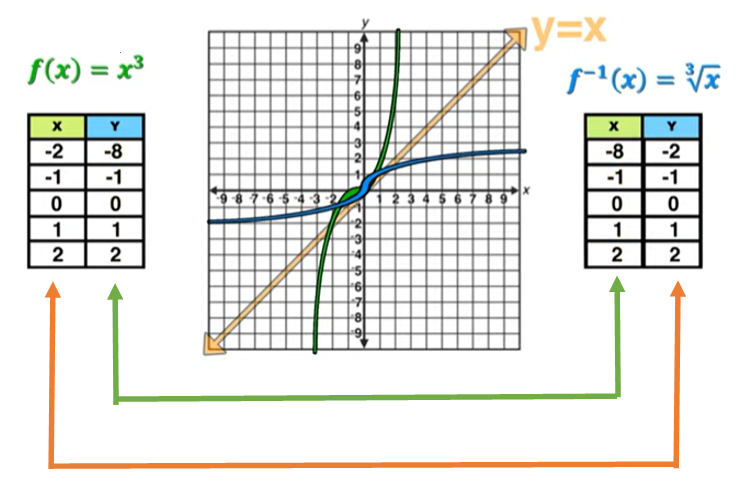
\includegraphics[width=0.6\linewidth]{img04/w04-InvFunDemo} \end{center}

The above table and figure basically show that we swap x- and y-coordinates of one function to get its inverse and the corresponding curves are symmetric with respect to \(y = x\), the diagonal of the first and third quadrants.

Algebraically, the above figure basically says that, to find the inverse of \(y = f(x)\) (if it exists), we only need to swap \(x\) and \(y\) in \(y = f(x)\) to get \(x = f(y)\). \textbf{\color{red}Keep in mind that \(y\) in \(x = f(y)\) is still the dependent variable and x is still the independent variable}.

In many cases, we want to re-express \(y\) explicitly in term of \(x\) as \(y = f^{-1}(x)\) \textbf{\color{red}if the close form exists}.

Next chart shows the steps for finding the explicit expression of an inverse function (if it exists).

\begin{center}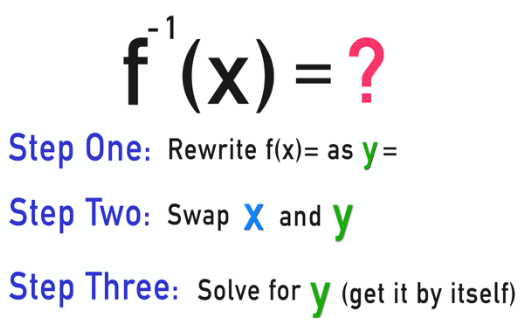
\includegraphics[width=0.45\linewidth]{img04/w04-inverseFun} \end{center}

\textbf{Example 1}. Find the inverse function of \(f(x) = x^2\) for \(x > 0\).

\textbf{Solution}: According to the steps, we have

\texttt{Step\ 1.} let \(y = x^2\).

\texttt{Step\ 2.} swap \(x\) and \(y\): \(x = y^2\).

\texttt{Step\ 3.} Solve for \(y\): \(y = \sqrt{x}\).

Therefore, the inverse of \(f(x) = x^2\) is given by \(y = f^{-1}(x) = \sqrt{x}\).

The following animated graph shows the symmetry of \(y = x^2\) and \(x = \sqrt{x}\).

\hfill\break

\url{https://github.com/pengdsci/MAT143/raw/main/w04/img/Function-inverse-animation2.gif}

\hfill\break

\hypertarget{definition-of-natural-base-euler-constant-e}{%
\section{\texorpdfstring{Definition of Natural Base (Euler Constant \(e\))}{Definition of Natural Base (Euler Constant e)}}\label{definition-of-natural-base-euler-constant-e}}

\hfill\break

\textbf{Example 2}. Assume that you put 10000 dollars (\textbf{principal}, denoted by \(P\)) in a saving account. The Bank pays you the interest at an annual rate of \(r\) (in decimal, for example, \(r = 2.5\% = 0.025\)) . We look at the number of times (\(n\)) the bank calculates the compounding interest \textbf{in a year} and the corresponding interest earnings. For convenience, we use \(A\) to denote the \textbf{acount balance} (the amount in the account after a year, i.e., \textbf{A = principal + interest}).

\begin{itemize}
\item
  \(n = 1\): A = principal (P) + interest (\(P\times r\)) = \(P + Pr = P(1+r)\).
\item
  \(n =2\): Since the bank will compound the interest two times a year. When calculating the interest, we need to use the semi-annual interest rate (\(r/2\)) instead of the original annual rate (\(r\)).

  \begin{itemize}
  \item
    First calculation: \(A_1 = P + P\times (r/2) = P(1 + r/2)\). Since the interest from every previous period is added to the principal, this means that \(A_1\) will be new principal in the second calculation;
  \item
    Second calculation: \(A_2 = A_1 + A_1 \times (r/2) = A_1(1+r/2) = P(1+r/2)\times (1 + r/2) = P(1 + r/2)^2\).
  \end{itemize}
\item
  \(n = 3\): Use the sample logic in the case of \(n = 2\), the interest rate in each of the three calculations is \(r/3\).

  \begin{itemize}
  \item
    First calculation: \(A_1 = P + P\times (r/3) = P(1 + r/3)\), This \(A_1\) will be new principal in the second calculation;
  \item
    Second calculation: \(A_2 = A_1 + A_1 \times (r/3) = A_1(1+r/3) = P(1+r/3)\times (1 + r/3) = P(1 + r/3)^2\).
  \item
    Third calculation: \(A_3 = A_2 + A_2 \times (r/3) = A_2(1+r/3) = P(1+r/3)^2\times (1 + r/3) = P(1 + r/3)^3\).
  \end{itemize}
\end{itemize}

In general, if the interest is compounded \(n\) times a year, then the balance is expressed in the following

\begin{center}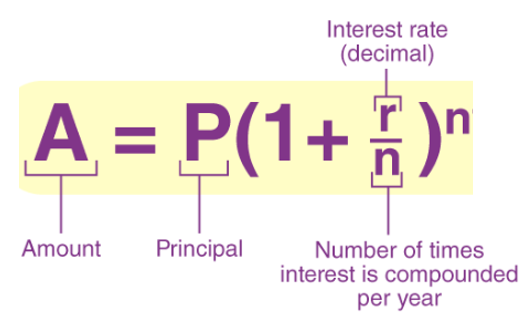
\includegraphics[width=0.45\linewidth]{img04/w04-CompundInterestOneYear} \end{center}

The above formula can be re-expressed into

\begin{center}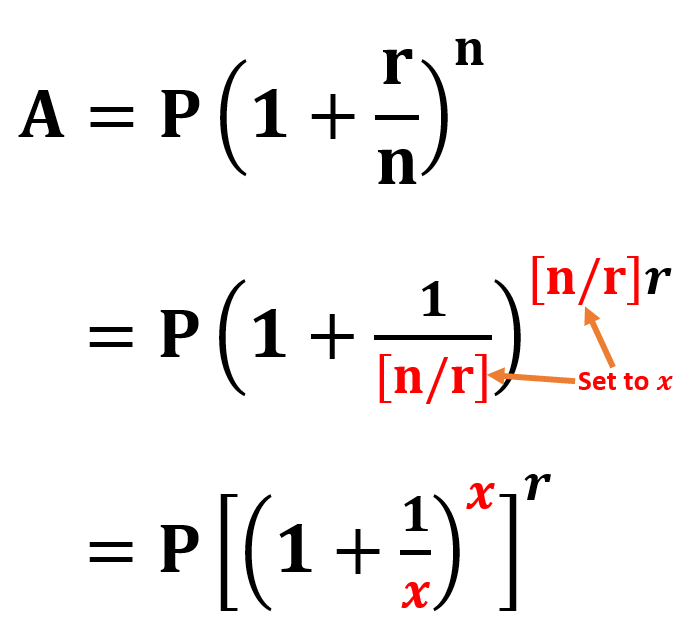
\includegraphics[width=0.6\linewidth]{img04/w04-CompoundingInterest02} \end{center}

\textbf{\color{red}If the interest is compounded continuously, i.e., \(n \to \infty\)}, then \textbf{\color{blue}\(x \to \infty\)}.

\hfill\break

\textbf{Definition}: The \textbf{natural base}, denoted by \(e\), is the \textbf{constant value} given by
\[
e = \lim_{x \to \infty}\left( 1 + \frac{1}{x}\right)^x \approx 2.71828182845....
\]

Therefore, if the interest is compounded continually, \textbf{\color{red}the account balance after a year} is simply expressed in the following form

\begin{center}
\includegraphics[width=0.3\linewidth]{img04/w04-AnnualBalanceContinuousCompounding} \end{center}

More generally, with principal \(P\) and continuous compounding interest, the account balance after \(y\) years is

\begin{center}\includegraphics[width=0.3\linewidth]{img04/w04-AnnualBalanceT-years-balance} \end{center}

where \(t = \text{ number of years}\). The component \(e^r\) is dependent on the value of the nominal annual interest rate. It is considered a function of \(r\) - natural base exponential function.

\hfill\break

\textbf{Example 3}: Rachel invests \$20,000 in an account that earns interest at an annual rate of 4\%. Find the future value of her account after 3 yr if interest is compounded continuously.

\textbf{Solution}: We have \(P =\$20000, r = 0.04\), and \(t = 3\). Since interest is compounded continuously, after 3 yr, Rachel's account will be worth

\[
A = 20000e^{0.04\times 3} = 23470.22.
\]
Therefore, the account balance after 3 years is \(\$23470.22\).

\hfill\break

\hypertarget{natural-base-exponential-and-logarithmic-functions}{%
\section{Natural-base Exponential and Logarithmic Functions}\label{natural-base-exponential-and-logarithmic-functions}}

The example in the previous section shows that various exponential growth and decay models in applications in the business and other fields are natural base exponential function. Next, we outline the natural base exponential function and its inverse, natural base exponential and logarithmic functions.

\begin{center}\includegraphics[width=0.6\linewidth]{img04/w04-NaturalExpLogDef} \end{center}

\hfill\break

The definition of natural base exponential and longarithmic functions are defined respectively in the following.

\hfill\break

\begin{center}\includegraphics[width=0.4\linewidth]{img04/w04-ExpLogNaturalComparison} \end{center}

Since \(y = e^x\) and \(y = \ln(x)\) are mutually inverse, their curves are symmetric with respect to \(y = x\).

\begin{center}\includegraphics[width=0.4\linewidth]{img04/w04-NaturalExpLog} \end{center}

The basic properties of natural logarithmic and exponential functions are summarized in the following.

\begin{center}\includegraphics[width=0.7\linewidth]{img04/w04-NaturalExpLogProperties} \end{center}

\textbf{Example 3}: Simply the following expressions.

\begin{enumerate}
\def\labelenumi{\arabic{enumi}.}
\item
  \(\ln(x^4\sqrt{x^5})\)
\item
  \(\ln(x^3y^2/z^5)\)
\end{enumerate}

\textbf{Solution}: We the above rules to simply the given expressions.

\begin{enumerate}
\def\labelenumi{\arabic{enumi}.}
\item
  \(\ln(x^4\sqrt{x^5}) = \ln(x^4 \times x^{5/2}) = \ln(x^{4+5/2}) = \ln(x^{13/2}) = (13/2)\ln(x)\)
\item
  \(\ln(x^3y^2/z^5) = \ln(x^3y^2) -\ln(z^5) = \ln(x^3) + \ln(y^2) - \ln(x^5) = 3\ln x+2\ln y -5\ln z\).
\end{enumerate}

\hypertarget{derivative-of-logarithmic-and-exponential-functions}{%
\chapter{Derivative of Logarithmic and Exponential Functions}\label{derivative-of-logarithmic-and-exponential-functions}}

\hypertarget{review-topics}{%
\section{Review Topics}\label{review-topics}}

\begin{itemize}
\tightlist
\item
  \textbf{Definitions of Log and Exponential Functions}
\end{itemize}

\begin{center}\includegraphics[width=0.4\linewidth]{img05/w05-ExpLogNaturalComparison} \end{center}

\begin{itemize}
\tightlist
\item
  The basic properties of natural logarithmic and exponential functions are summarized in the following.
\end{itemize}

\begin{center}\includegraphics[width=0.7\linewidth]{img05/w05-NaturalExpLogProperties} \end{center}

\textbf{Example 1}:

\begin{itemize}
\item
  Five Rules of Derivative

  \begin{enumerate}
  \def\labelenumi{\arabic{enumi}.}
  \item
    \textbf{Power Rule}: \([x^a]^\prime = a x^{a-1}\).
  \item
    \textbf{Additive Rule}: \([f(x) + g(x)]^\prime = f^\prime(x) + g^\prime(x)\).
  \item
    \textbf{Multiplicative Rule}: \([f(x)g(x)]^\prime = f^\prime(x)g(x) + f(x)g^\prime(x)\).
  \item
    \textbf{Quotient Rule}: \([f(x)/g(x)]^\prime = [f^\prime(x)g(x) - f(x)g^\prime(x)]/g^2(x)\).
  \item
    \textbf{Chain Rule}: \([f\circ g (x)]^\prime = f^\prime[g(x)] g^\prime(x)\).
  \end{enumerate}

  \textbf{Example 2}: (1). \(f_1(x) = \sqrt[5]{x^3}\), (2). \(f_2(x) = (x^2+1)\sqrt{x}\), (3). \(f_3(x) = x^2/(x+1)\), (4). \(f_4(x) = (1/x+1)^2\)
\end{itemize}

\hfill\break

\hypertarget{derivative-of-natural-base-exponential-functions}{%
\section{Derivative of Natural-base Exponential Functions}\label{derivative-of-natural-base-exponential-functions}}

\hfill\break

\textbf{Theorem 1}: Let \(f(x) = e^x\), then \(f^\prime(x) = [e^x]^\prime = e^x\).

\hfill\break

\begin{center}\includegraphics[width=0.7\linewidth]{img05/w05-derivativeExp} \end{center}

\textbf{Example 1}: Find the derive of the following functions (that contains \(e^x\)).

(1). \(y = 3e^x\)

(2). \(f(x) = x^2e^x\)

(3). \(h(x) = e^x/x^3\)

\textbf{Solution}: Each of the above functions contains more than one component. To find the derivative of these functions, we need to use rule \([e^x]^\prime = e^x\) and other rules of derivative as well.

(1). \(y\) involves scalar multiplication. \(y^\prime = [3e^x]^\prime = 3[e^x]^\prime = 3e^x\).

(2). \(f(x)\) is a product of two functions. \(f^\prime(x) = [x^2e^x]^\prime = [x^2]^\prime e^x + x^2 [e^x]^\prime = 2xe^x + x^2e^x=x(2+x)e^x\)

(3). \(h(x)\) is a fractional function. \(h^\prime(x) = [e^x/x^3]^\prime = [(e^x)^\prime x^3 - e^x(x^3)^\prime]/x^6 = (x - 3)e^x/x^4\)

\hfill\break

The problems in the above example contain \(e^x\) as a component. Recall that the compounding interest example we discussed earlier has the general form \(A(t) = Pe^{rt}\), where \(A(t)\) is the account balance at the end of \(t\) years, \(r\) is the annual rate, \(t\) is the number of years of investment. This investment function contains \(e^{rt}\). We need to know the derivative of \(f(x) = e^{g(x)}\), where \(g(x)\) is differentiable (i.e., the derivative of \(g(x)\) exists).

\textbf{Theorem 2}: Let \(f(x) = e^{g(x)}\), then \(f^\prime(x) = [e^{g(x)}]^\prime = e^{g(x)}\times g^\prime(x)\).

\hfill\break

The above theorem is essentially an application of the \textbf{chain rule} to the general natural base exponential function. The following figure illustrated the use of the above theorem with an example.

\hfill\break

\begin{center}\includegraphics[width=0.7\linewidth]{img05/w05-derivativeCompositeExp} \end{center}

\hfill\break
\textbf{Example 3}: Find the derivative of the following functions.

(1). \(f(x) = e^{8x}\)

(2). \(f(x) = e^{-x^2 + 4x -7}\)

(3). \(f(x) = e^{\sqrt{x^2-3}}\)

\textbf{Solution}: We need to use result in \textbf{Theorem 2} and other rules of derivative.

(1). \(f^\prime(x) = [e^{8x}]^\prime = e^{8x}\times (8x)^\prime = 8e^{8x}\).

(2). \(f^\prime(x) = [e^{-x^2 + 4x -7}]^\prime = e^{-x^2 + 4x -7}(-x^2 + 4x -7)^\prime = 2(2-x)e^{-x^2 + 4x -7}\)

(3). \(f^\prime(x) = [e^{\sqrt{x^2-3}}]^\prime = e^{\sqrt{x^2-3}}\times(\sqrt{x^2-3})^\prime\)

\(=e^{\sqrt{x^2-3}}\times [(x^2-3)^{1/2}]^\prime =e^{\sqrt{x^2-3}}\times (1/2)\times (x^2-3)^{1/2-1}(x^2-3)^\prime\)

\(=\frac{1}{2}e^{\sqrt{x^2-3}}\times (x^2-3)^{-1/2}\times(2x) = \frac{xe^{\sqrt{x^2-3}}}{\sqrt{x^2-3}}\)

\textbf{Example 4}: Franco's Fishing Emporium invested \$50,000 in an account that earns 1.25\% annual interest, compounded continuously. The value of the account after \(t\) years is given by

\[
A(t) = 50000e^{0.0125t}
\]

Find \(A(5)\) and \(A^\prime(5)\) and interpret the meaning of each of these values.

\textbf{Solution}: To find \(A(5)\), we simply substitute \(t = 5\) n \(A(t)\) that gives
\[
A(5) = 50000e^{0.0125\times 5} \approx 53224.72.
\]
Note that,

\begin{center}\includegraphics[width=0.7\linewidth]{img05/w05-EvaluateDerivative} \end{center}

The derivative \(A^\prime(t)\) can be found in the following.

\begin{center}\includegraphics[width=0.7\linewidth]{img05/w05-BalanceFunDerivative} \end{center}

\hfill\break
Therefore,\\

\begin{center}\includegraphics[width=0.7\linewidth]{img05/w05-BalanceFunDA(5)} \end{center}

After exactly 5 yr, the value of Franco's Fishing Emporium's account is \$53,224.72, and at that instant, the value is growing at the rate of \$665.31 per year.

\hfill\break

\hypertarget{derivative-of-natural-logarithmic-functions}{%
\section{Derivative of Natural Logarithmic Functions}\label{derivative-of-natural-logarithmic-functions}}

\hfill\break

Note that \(f(x) = \ln(x)\) is equivalent to \(e^{f(x)} = x\). Taking the derivative of both sides of the above equation, we have

\[
[e^{f(x)}]^\prime = [x]^\prime
\]
that is equivalent to

\[
f^\prime(x) e^{f(x)} = 1, \ \ \text{ that is, } \ \ x f^\prime(x) = 1 \ \ \text{ since } e^{f(x)} = x.
\]

Therefore,

\[
f^\prime(x) = [\ln(x)]^\prime = \frac{1}{x}.
\]
Using the same steps, we have

\[
[\ln f(x)]^\prime = \frac{f^\prime(x)}{f(x)}.
\]

In summary, we have the following formulas

\begin{center}\includegraphics[width=0.7\linewidth]{img05/w05-derivativeLog} \end{center}

\textbf{Example 5} Find the derivative of the following functions

(1). \(y = 3\ln (x)\).

(2). \(y = x^2/\ln (x)\).

(3). \(y = x^4\ln(x) + 5x\)

\textbf{Solution}: We will use the above theorem and the five rules (power rule, scalar multiplication, additive, multiplicative, quotient, and chain rules) of derivatives as well.

(1). \(y^\prime = [3\ln (x)]^\prime = 3[\ln (x)]^\prime = 3\times \frac{1}{x} = \frac{3}{x}\).

(2). \(y^\prime = [x^2/\ln (x)]^\prime = \frac{[x^2]^\prime \ln(x) - x^2[\ln(x)]^\prime}{[\ln(x)]^2} = \frac{2x\ln(x)-x^2(1/x)}{[\ln(x)]^3} = \frac{x[2\ln(x)-1]}{[\ln(x)]^2}\).

(3). \(y^\prime = [x^4\ln(x) + 5x]^\prime = [x^4\ln(x)]^\prime + [5x]^\prime = [x^4]^\prime\ln(x) + x^4[\ln(x)]^\prime + 5\)

\(= 4x^3\ln(x) + x^4(1/x) + 5 = 4x^3\ln(x) + x^3 + 5 = x^3[4\ln(x)+1]+ 5\)

\hfill\break

\textbf{Example 6}: Find the derivative of the following functions.

(1). \(y = \ln(x^2-1)\)

(2). \(f(x) = \ln[(x^3 + 4)/x]\)

\textbf{Solution}: We need the chain rule (the second part of the theorem) and other rules of derivative.

(1). \(y^\prime = [\ln(x^2-1)]^\prime = \frac{(x^2-1)^\prime}{x^2-1} = \frac{2x}{x^2-1}\)

(2). \textbf{Method 1}: We start with the chain rule. \(f^\prime(x)= \{\ln[(x^3 + 4)/x]\}^\prime = \frac{[(x^3 + 4)/x]^\prime}{(x^3 + 4)/x} = \frac{([(x^3 + 4)^\prime x- (x^3+4)(x)^\prime]/x^2}{(x^3 + 4)/x}\)

\(= \frac{([3x^3\times x- (x^3+4)]/x^2}{(x^3 + 4)/x} = \frac{3x^4- x^3-4}{x(x^3 + 4)}\)

\textbf{\color{red}We can use the property of the logarithmic function to simplify the given function and then take the derivative.}

\textbf{Method 2}: We simplify the function before taking derivatives. \(f^\prime(x)= \{\ln[(x^3 + 4)/x]\}^\prime = [\ln(x^3 + 4) - \ln(x)]^\prime\)

\(= [\ln(x^3+4)]^\prime -[\ln(x)]^\prime= \frac{(x^3+4)^\prime}{x^3+4} +\frac{1}{x} = \frac{3x^2}{x^3+4} - \frac{1}{x} = \frac{3x^3-x^3-4}{x(x^3+4)}\)

\hfill\break

\textbf{Example 7}: \textbf{Marginal Cost}. Suppose \(C(x)\) is the total cost of producing \(x\) skateboards and

\[
C(x) = 1800 + 10x + 0.02x^2 \ \text{dolloars}
\]
(1). Find the marginal cost function.

(2). Find the marginal cost at \(x= 500\) and interpret the result.

\textbf{Solution}: Before answering the above two questions, we need to know \textbf{what the marginal cost is} and \textbf{how the marginal cost is defined}. The following figure defines the marginal cost.

\begin{center}\includegraphics[width=0.8\linewidth]{img05/w05-MarginalCost} \end{center}

\begin{quote}
The marginal revenue, cost, and profit functions are what the company can use to determine whether or not it should increase production. These marginal functions are the derivatives of their associated functions. So
\end{quote}

\begin{quote}
the \emph{marginal revenue function is the derivative of the revenue function, \(MR(x) = R^\prime(x)\)};
\end{quote}

\begin{quote}
the \emph{marginal cost function is the derivative of the cost function, \(MC(x) = C^\prime(x)\)};
\end{quote}

\begin{quote}
the \emph{marginal profit function is the derivative of the profit function, \(MP(x) = P^\prime(x)\)}.
\end{quote}

\textbf{\color{red}With the above concepts of marginal cost, we now answer the above questions.}

(1). The marginal cost function, denoted by \(MC(x)\), is given by

\[
MC(x) = C^\prime(x) = [1800 + 10x + 0.02x^2]^\prime = 10 + 0.04x
\]

(2). \(C^\prime(500) = 10 + 0.04\times 500 = 10 + 20 = 30\). This means, at the current production capacity (of producing 500 items), producing one additional item will increase an additional \$30 cost.

\hfill\break

\hypertarget{exponential-models}{%
\section{Exponential Models}\label{exponential-models}}

The follow theorem defines a very commonly used exponential models.

\hfill\break

\begin{center}\includegraphics[width=0.6\linewidth]{img05/w05-ExponentialGrowthModel} \end{center}

\hfill\break

If \(k > 0\), the corresponding model is called \textbf{exponential growth model}. If \(k < 0\), the exponential model is called \textbf{exponential decay model}.

\hypertarget{exponential-growth-model}{%
\subsection{Exponential Growth Model}\label{exponential-growth-model}}

Consider the investment function in \textbf{Example 4}, \(A(t) = 50000e^{0.0125t}\), where \(t\) is the number of years. We also calculated the derivative \(A^\prime(t) =0.0125 \times 5000e^{0.0125t}\).

Observe that \(A^\prime(t)\) and \(A(t)\) have a direct relationship: \(A^\prime(t) = 0.0125A(t)\). In general, if a function \(y = f(x)\) that \(f^\prime(x) = k f(x)\) (\(k\) is a constant), we call it the \textbf{exponential growth} model. We formalized this observation in the following theorem (without proving it)

If \(k > 0\), the corresponding exponential growth model has no upper bound. It is usually called the \textbf{uninhibited Population Growth Model}. The constant \(c\) is the initial value at \(t = 0\).

\hfill\break

\textbf{Example 8}: Business: Interest Compounded Continuously. Suppose \(P_0\), in dollars, is invested in the Von Neumann Hi-Yield Fund, with interest compounded continuously at \(7%
\) per year. That is, at any point in time after \(t\) years, the balance \(P\), in dollars per year, is growing at the rate

\[
\frac{dP(t)}{dt}=0.07P(t)
\]

\textbf{(a)}. Find the function that satisfies the equation. Write it in terms of \(P_0\) and 0.07.

\textbf{(b)}. Suppose that \$10,000 is invested. What is the balance after 1 yr?

\textbf{(c)}. If \$10,000 is invested, how fast is the balance growing at \(t=1\) year?

\textbf{Solution}. Use the above Theorem 3 and a calculator to answer the three questions.

\textbf{(a)}: According to the theorem, \(P(t) = P_0 e^{0.07t}\)

\textbf{(b)}: Since \(P(t) = 10000e^{0.07t}\), therefore, \(P(1) = 10000e^{0.07\times 1} = 10000e^{0.07} \approx 10725.0818125422 \approx 10725.08 \text{ dollars}\).

\textbf{(c)}: Since \(P^\prime(t) = 10000e^{0.07t}\times 0.07 = 700e^{0.07t}\). Therefore, \(P^\prime(1) = 700e^{0.07\times 1} = 700e^{0.07} \approx 750.755726877952 \approx =750.76\) dollars. At \(t = 1\), the balance is growing at the rate of about \$750.76 per year.

\hfill\break

\hypertarget{exponential-decay-models}{%
\subsection{Exponential Decay Models}\label{exponential-decay-models}}

\textbf{Example 9} \textbf{Population decay}. Since 1980, the population of Trenton, New Jersey, has been decreasing by \(2.72\%\) per year. The rate of change of the city's population P, t years after 1980, is given by

\[
\frac{dP}{dt} = -0.0272
\]

In 1980, the population of Trenton was 92,124. (Source: U.S. Census Bureau.)

(a). Find an exponential function that models this situation.

(b). What is the rate of change of the population of Trenton in 2030?

\textbf{Solution}: By the above

\hypertarget{derivative-of-general-logarithmic-and-exponential-functions}{%
\chapter{Derivative of General Logarithmic and Exponential Functions}\label{derivative-of-general-logarithmic-and-exponential-functions}}

This note discusses the derivative of logarithmic and exponential functions with arnitrary bases.

\hypertarget{review-topics-1}{%
\section{Review Topics}\label{review-topics-1}}

We first review some concepts and properties learned in algebra and the rules of derivative we learned in the past few weeks.

\hfill\break

\hypertarget{five-rules-of-derivative}{%
\subsection{Five Rules of Derivative}\label{five-rules-of-derivative}}

\hfill\break

These rules of derivative will be used frequently throughout the semester.

\begin{center}\includegraphics[width=0.8\linewidth]{img06/w06-RuelDerivatives} \end{center}

\hfill\break

\hypertarget{log-and-exponential-functions---definitions}{%
\subsection{Log and Exponential Functions - Definitions}\label{log-and-exponential-functions---definitions}}

We review the definitions of exponential and logarithmic functions with any arbitrarily given valid bases.\\

\begin{center}\includegraphics[width=0.7\linewidth]{img06/w06-GenLogExp-Def} \end{center}

The two functions are mutually inverse just like we explained for natural based exponential an logarithmic functions.

\hfill\break

\hypertarget{log-and-exponential-functions---properties}{%
\subsection{Log and Exponential Functions - Properties}\label{log-and-exponential-functions---properties}}

The following properties are very useful in simplifying the given functions, particularly the last two properties that are used used to derive the derivatives of the general exponential and logarithmic functions.

\hfill\break

\begin{center}\includegraphics[width=0.8\linewidth]{img06/w06-GenLogExp-Properties} \end{center}

Here are some examples

(1). Change the base of logarithm expression to natural base: (a) \(\log_{10} 15\), (b) \(\log_5 e^2\)

(2). Change the exponential expression to a natural base exponential expression: (a) \(3^5\), (b) 10\^{}(-4)

\hfill\break

\hypertarget{derivative-of-natural-base-functions}{%
\subsection{Derivative of Natural-base Functions}\label{derivative-of-natural-base-functions}}

\hfill\break

\begin{center}\includegraphics[width=0.8\linewidth]{img06/w06-DerivativesExpLn} \end{center}

\hfill\break

\textbf{Example 1}: The profit, in thousands of dollars, from the sale of x thousand candles can be estimated by

\[
P(x) = e^{2x} - 0.3x \ln(x+1)
\]

Find the marginal profit \(P^\prime(3)\) and interpret the result.

\textbf{Solution}:

\begin{center}\includegraphics[width=0.8\linewidth]{img06/w06-ReviewExample01} \end{center}

\[
P^\prime(x) = [e^{2x} - 0.3x\ln(x+1)]^\prime = [e^{2x}]^\prime - 0.3[x\ln(x+1)]^\prime
\]

\[
=e^{2x}[2x]^\prime - 0.3\left\{(x)^\prime \ln(x+1) + x[\ln(x+1)]^\prime\right\}
\]

\[
= 2e^{2x}-0.3\ln(x+1) + \frac{0.3x}{x+1}.
\]

Therefore,

\[
P^\prime(3) = 2e^6 - 0.3\ln(1+3) + \frac{0.9}{1+3} \approx 806.67.
\]
The marginal profit is 806.67 (i.e., selling 1000 more candles will make additional profit of \$806.67.

\hfill\break

\hypertarget{exponential-and-logarithmic-functions}{%
\section{Exponential and Logarithmic Functions}\label{exponential-and-logarithmic-functions}}

\textbf{Example 2}. It is known that 49.4\% of all aluminum cans distributed are recycled each year. A beverage company uses 250,000 lb of aluminum cans. After recycling, the amount of aluminum, in pounds, still in use after t years is given by

\[
N(t) = 250000\times 0.494^t
\]

Find \(N^\prime(3)\) and explain its meaning.

\hfill\break

Function \(N(t)\) involves a term \(0.494^t\). This is NOT a power function! This is also NOT the natural base exponential function. In general, we want to have formulas to calculate the derivative of the exponential and logarithmic functions with any arbitrary bases (bigger than 0 and not equal to 1).

In fact, the derivative of \(a^x\) and \(\log_a(x)\) can be easily derive using the change base properties and chain rule of natual log and exponential functions.

\[
[a^x]^\prime = [e^{\ln(a)x}]^\prime = e^{\ln(a) x}\times[\ln(a)x]^\prime = a^x\ln(a)
\]

and

\[
[\log_a(x)]^\prime = \left[ \frac{\ln(x)}{\ln(a)}\right]^\prime = \frac{1}{\ln(a)}[\ln(x)]^\prime = \frac{1}{\ln(a)}\frac{1}{x} = \frac{1}{x\ln(a)}.
\]

We can similarly find the following more general results (chain rule for general exponential and logarithmic functions).

\[
\left[a^{f(x)}\right]^\prime =\left[e^{\ln(a)f(x)}\right]^\prime  = e^{\ln(a)f(x)}\times [\ln(a)f(x)]^\prime =\ln(a) a^{f(x)}\times f^\prime(x) 
\]
and

\[
[\ln(f(x))]^\prime = \left[ \frac{\ln f(x)}{\ln(a)}\right]^\prime = \frac{1}{\ln(a)}[\ln f(x)]^\prime = \frac{1}{\ln(a)}\frac{f^\prime(x)}{f(x)} = \frac{f^\prime(x)}{\ln(a)f(x)}
\]

In summary, we have

\begin{center}\includegraphics[width=0.8\linewidth]{img06/w06-DerivativeExploga} \end{center}

\textbf{Example 3}: Find the derivative of the following functions.

\begin{enumerate}
\def\labelenumi{(\arabic{enumi})}
\item
  \(y = 2^x\)
\item
  \(y = (1.4)^x\)
\item
  \(y = 3^{2x + 1}\)
\item
  \(y = \log_8 x\)
\item
  \(y = \log_3 (x^2 + 1)\)
\item
  \(y = x^3 \log_5(x)\)
\end{enumerate}

\textbf{Solution}: We will the above rules and other rules of derivatives to calculate the derives.

\begin{center}\includegraphics[width=0.8\linewidth]{img06/w06-Advice} \end{center}

\begin{enumerate}
\def\labelenumi{(\arabic{enumi})}
\item
  \(y^\prime = [2^x]^\prime = \ln(2) 2^x\)
\item
  \(y^\prime = [1.4^x]^\prime = 1.4^x \ln(1.4)\)
\item
  \(y^\prime = [3^{2x+1}]^\prime = \ln(3)3^{2x+1}\times(2x+1)^\prime = 2\ln(3) 3^{2x+1}\)
\item
  \(y^\prime = [\log_8(x)]^\prime = \frac{1}{x \ln(8)}\)
\item
  \(y^\prime = [\log_3(x^2+1)]^\prime = \frac{(x^2+1)^\prime}{(x^2+1)\ln(3)} = \frac{2x}{(x^2+1)\ln(3)}\)
\item
  \(y^\prime = [x^3\log_5(x)]^\prime = [x^3]^\prime \log_5(x) + x^3 [\log_5(x)]^\prime = 3x^2\log_5(x) + x^3\frac{1}{x\ln(5)} = 3x^2\log_5(x) + \frac{x^3}{x\ln(5)}\)
\end{enumerate}

\hfill\break

\hypertarget{business-applications}{%
\section{Business Applications}\label{business-applications}}

This section uses several examples to show various business applications of exponential models.

\textbf{Example 4} Irma invested \$15,000 in a high-yield hedge fund, and after 14 yr, her original investment has tripled. Find exponential functions using base 3 and base e that give the value A of her account after \(t\) years. What is the yearly percentage growth rate of her fund? Which exponential function is easier to use to find this information?

\textbf{Solution}: Using base 3 \((n = 3)\) and a tripling time of \(T = 14\), we have

\[
A(t) = 15000\times 3^{t/14}
\]

In base e, this is equivalent to

\[
A(t) = 15000\times(e^{\ln3})^{t/14} \approx 15000 e^{0.0785t}
\]
The above expression means that Irma's hedge fund has a yearly percentage growth rate of 7.85\%. Using the function with base e, we can read this value directly from the exponent.

\textbf{Example 5: Double declining balance depreciation}. An office machine is purchased for \$5200. Assume that its salvage value, V, in dollars, depreciates, according to a method called double declining balance, by 20\% each year and is given by

\[
V(t) = 5200(0.80)^t
\]

where t is the time, in years, after purchase. Find \(V^\prime(5)\), and explain its meaning.

\textbf{Solution}: We first find the derivative of \(V(t)\).

\[
V^\prime(t) = [5200(0.8)^t]^\prime = 5200[0.8^t]^\prime = 5200\times \ln(0.8)\times 0.8^t = -1160.346\times 0.8^t
\]
Therefore,

\[
V^\prime(5) = -1160.346\times 0.8^5 \approx -380.2223
\]
Therefore, the declining rate at the end of year 5 is about \(\$380\).

\hfill\break

\textbf{Example 6}: Agriculture. Farmers wishing to avoid the use of nonheirloom seeds are increasingly concerned about inadvertently growing nonheirloom plants as a result of pollen drifting from nearby farms. Assuming that these farmers raise their own seeds, the fractional portion of their crop that remains free of nonheirloom plants t years later can be approximated by

\[
P(t) = (0.98)^t
\]
1. Using this model, predict the fractional portion of the crop that will be nonheirloom 10 yr after a neighboring farm begins to use nonheirloom seeds.

\textbf{Solution}: We simply evaluate the original function.

\[
P(t) = 0.98^{10} \approx 0.8171 = 81.71\%.
\]

\begin{enumerate}
\def\labelenumi{\arabic{enumi}.}
\setcounter{enumi}{1}
\tightlist
\item
  Find \(P^\prime(10)\) and explain its meaning.
\end{enumerate}

\textbf{Solution}: We find the derivative \(P^\prime(t)\) first in the following

\[
P^\prime(t) = [0.98^t]^\prime = \ln(0.98)\times 0.98^t = -0.02020271\times 0.98^t.
\]

Therefore,

\[
P^\prime(10) = -0.02020271\times 0.98^{10} =  -0.01650708.
\]

Therefore, at the end of year 10, the decreasing rate is about \(1.65\%\).

\textbf{Example 7} Following the birth of their granddaughter, Doug and Andrea want to make an initial investment, \(P_0\), that will grow to \$10,000 by the child's 20th birthday. Interest is compounded continuously at an annual rate of 4\%. What should the initial investment be?

\hypertarget{critical-values}{%
\chapter{Critical Values}\label{critical-values}}

As an application of the derivative, we discuss the concept of critical value and its real-world applications in this note.

\hypertarget{review-topics-2}{%
\section{Review Topics}\label{review-topics-2}}

We first review the Five Rules of Derivative that will be used frequently throughout the semester.

\begin{center}\includegraphics[width=0.8\linewidth]{img07/w07-RuleDerivatives} \end{center}

\hfill\break

We will apply derivatives to solve real-world optimization problems maximizing profit or revenue and minimizing the cost, etc. This note focuses on the concepts of critical values and using derivation to find critical values.

\hfill\break

\hypertarget{increasing-and-decreasing-functions}{%
\section{Increasing and decreasing functions}\label{increasing-and-decreasing-functions}}

We reviewed monotonic function in the first week. The following figures demonstrate increasing and decreasing functions.

\begin{center}\includegraphics[width=0.8\linewidth]{img07/w07-MonotonicFunctions} \end{center}

Using the definition of the derivative, we can see that

\begin{itemize}
\item
  If \(f(x)\) is increasing over \([a, b]\), then \(f^\prime(x) > 0\) over \([a, b]\);
\item
  If \(f(x)\) is decreasing over \([a, b]\), then \(f^\prime(x) < 0\) over \([a, b]\).
\end{itemize}

Graphically, we have the following figures explain the above observation

\begin{center}\includegraphics[width=0.8\linewidth]{img07/w07-DerivativeVSmonotonicity} \end{center}

We next formalize the above observation and present the following theorem.

\textbf{Theorem 1}: Let \(f(x)\) be differential over interval \(I = [a,b]\)

\begin{enumerate}
\def\labelenumi{\arabic{enumi}.}
\item
  If \(f^\prime(x) > 0\) for all x in \(I = [a, b]\), then \(f(x)\) is increasing over \(I=[a, b]\)
\item
  If \(f^\prime(x) < 0\) for all x in \(I = [a, b]\), then \(f(x)\) is deceasing over \(I=[a,b]\).
\end{enumerate}

\textbf{Example 1}: Using the above Theorem 1 to find the intervals on which the function \(f(x) = x^3/3 - x + 2/3\).

\textbf{Solution}: The following figure answers the above question.

\begin{center}\includegraphics[width=0.6\linewidth]{img07/w07-increasingDecreasingIntervals} \end{center}

\hfill\break

\hypertarget{critival-value}{%
\section{Critival Value}\label{critival-value}}

In the above curve, two points A and B are special because the monotonicity of the function changed at these points (from increasing to decreasing at A and from decreasing to increasing at B). If the derivative of a function exists over an interval \([a, b]\), if the function changes its monotonicity, its sign of derivative also changes. That means, there exists a value, say \(c\), in \([a, b]\) that satisfies \(f^\prime(c) = 0\).

\begin{center}\includegraphics[width=0.6\linewidth]{img07/w07-CriticalValues} \end{center}

\textbf{Definition}: A \textbf{critical value} of a function \(f(x)\) is any number \(c\) in the \textbf{domain} of \(f(x)\) for which the tangent line at \((c, f(c))\) is horizontal or for which the derivative does \textbf{not} eixst. That is, \(c\) is a \textbf{critical} value if \(f(c)\) exists and

\[
f^\prime(c) = 0 ~ ~ \text{or}~~ f^\prime(c) ~ \text{does not exist}
\]
If \(c\) is a critical value of \(f(x)\), then \((c, f(c))\) is called a \textbf{critical point}.

\begin{center}\includegraphics[width=0.5\linewidth]{img07/w07-CriticalValues02} \end{center}

All labeled points on the above figure are critical points since the corresponding derivative is either 0 or does not exist.

\begin{enumerate}
\def\labelenumi{\arabic{enumi}.}
\item
  \(f^\prime(x) = 0\) for \(x = c_1, c_2, c_4, c_7\) and \(c_8\). That is, the tangent line to the graph is horizontal at these values.
\item
  \(f^\prime(x)\) does not exist for \(x = c_3, c_5\) and \(c_6\). The tangent line is vertical at \(c_3\) and there are corners at both \(c_5\) and \(c_6\).
\end{enumerate}

\textbf{Example 2} Find critical values of the function \(f(x) = x^3/3 - x + 2/3\).

\textbf{Solution}: By the definition, we need to the solution to \(f^\prime(x) = 0\) and those values on which the derivative of \(f(x)\) does not exist.

Note that \(f^\prime(x) = x^2 - 1\). Therefore, equation \(x^2 -1 = 0\) has solutions \(x = \pm 1\). These two critical values are the same as shown in example 1.

\hfill\break

\hypertarget{relative-local-maximum-and-minimum-values}{%
\section{Relative (Local) Maximum and Minimum Values}\label{relative-local-maximum-and-minimum-values}}

Graphically, the local maximum and minimum are the second coordinates of the points that are labeled in the following figure.

\begin{center}\includegraphics[width=0.6\linewidth]{img07/w07-localMinMax} \end{center}

Here, \(f(c_2)\) and \(f(c_4)\) are each an example of a \textbf{relative}, or \textbf{local}, \textbf{maximum (plural: maxima)}, and \(f(c_1), f(c_3)\) and \(f(c_5)\) are each an example of a relative, or local, \textbf{minimum (plural: minima)}. Collectively, maximum and minimum values are called \textbf{extrema (singular: extremum)}. Note that a relative minimum can be greater than a relative maximum; for example, \(f(c_5) > f(c_2)\) in the graph at the bottom of the preceding page.

Note that x-values at which a continuous function has relative extrema are those values for which the derivative is 0 or for which the derivative does not exist---the critical values.

\hfill\break
\textbf{Theorem}: If a function \(f(x)\) has a relative extreme value \(f(c)\) on an \textbf{open interval}, then \(c\) is a critical value, and

\[
f^\prime(c) = 0 ~~\text{or}~~f^\prime(c) ~~ \text{does not exist.}
\]

The next theorem gives a test for relative extrema: \textbf{The First-Derivative Test for Relative Extrema}

\hfill\break

\textbf{Theorem}: For any continuous function \(f(x)\) that has exactly one critical value \(c\) over an \textbf{open interval} \((a, b)\):

\begin{enumerate}
\def\labelenumi{\arabic{enumi}.}
\item
  \(f(x)\) has a relative minimum at \(c\) if \(f^\prime(x) < 0\) on \((a, c)\) and \(f^\prime(x) > 0\) on \((c, b)\). That is, \(f(x)\) is decreasing to the left of \(c\) and increasing to the right of \(c\).
\item
  \begin{enumerate}
  \def\labelenumii{\arabic{enumii}.}
  \tightlist
  \item
    \(f(x)\) has a relative maximum at \(c\) if \(f^\prime(x) > 0\) on \((a, c)\) and \(f^\prime(x) < 0\) on \((c, b)\). That is, \(f(x)\) is increasing to the left of \(c\) and decreasing to the right of \(c\).
  \end{enumerate}
\item
  \(f(x)\) has neither a relative maximum nor a relative minimum at \(c\) if \(f^\prime(x)\) has the same sign on both sides of \(c\).
\end{enumerate}

\textbf{Example 3}: Consider the relative maximum and relative minimum of function \(f(x) = 4x^3 - 9x^2 - 30x + 25\).

\textbf{Solution} The derivative \(f^\prime(x) = 12x^2 - 18x -30 = 6(2x^2 - 9x - 5) = 6(ax-5)(x+1)\). Set \(f^\prime(x) = 0\), we have \(6(ax-5)(x+1) = 0\), therefore, \(x = 2.5\) or \(x = -1\).

\begin{center}\includegraphics[width=0.6\linewidth]{img07/w07-extrema} \end{center}

\hfill\break

\hypertarget{critical-values-extema-and-curve-sketching}{%
\chapter{Critical Values, Extema and Curve Sketching}\label{critical-values-extema-and-curve-sketching}}

We first review the Five Rules of Derivative

\hfill\break

These rules of the derivative will be used frequently throughout the semester.

\begin{center}\includegraphics[width=0.99\linewidth]{img08/w08-RuleDerivatives} \end{center}

We also discussed the relationship between the monotonicity and the sign of the derivative of a function. The following figure summarizes the relationship.

\begin{center}\includegraphics[width=0.85\linewidth]{img08/w08-monotonicitySignDerivatives} \end{center}

\hfill\break

\hypertarget{summary-of-critical-values-and-extrema}{%
\section{Summary of Critical Values and Extrema}\label{summary-of-critical-values-and-extrema}}

\hfill\break

\hypertarget{critical-values-1}{%
\subsection{Critical values}\label{critical-values-1}}

\textbf{Definition}: A \textbf{critical value} of a function \(f(x)\) is any number \(c\) in the \textbf{domain} of \(f(x)\) for which the tangent line at \((c, f(c))\) is horizontal or for which the derivative does \textbf{not} eixst. That is, \(c\) is a \textbf{critical} value if \(f(c)\) exists and

\[
f^\prime(c) = 0 ~ ~ \text{or}~~ f^\prime(c) ~ \text{does not exist}
\]
If \(c\) is a critical value of \(f(x)\), then \((c, f(c))\) is called a \textbf{critical point}.

\begin{center}\includegraphics[width=0.7\linewidth]{img08/w08-criticalValues} \end{center}

All labeled points on the above figure are critical points since the corresponding derivative is either 0 or does not exist.

\begin{enumerate}
\def\labelenumi{\arabic{enumi}.}
\item
  \(f^\prime(x) = 0\) for \(x = c_1, c_2, c_4, c_7\) and \(c_8\). That is, the tangent line to the graph is horizontal at these values.
\item
  \(f^\prime(x)\) does not exist for \(x = c_3, c_5\) and \(c_6\). The tangent line is vertical at \(c_3\) and there are corners at both \(c_5\) and \(c_6\).
\end{enumerate}

\textbf{Example 2} Find critical values of the function \(f(x) = x^3/3 - x + 2/3\).

\textbf{Solution}: By the definition, we need to the solution to \(f^\prime(x) = 0\) and those values on which the derivative of \(f(x)\) does not exist.

Note that \(f^\prime(x) = x^2 - 1\). Therefore, equation \(x^2 -1 = 0\) has solutions \(x = \pm 1\). These two critical values are the same as shown in example 1.

\hfill\break

\hypertarget{relative-local-maximum-and-minimum-values-1}{%
\subsection{Relative (Local) Maximum and Minimum Values}\label{relative-local-maximum-and-minimum-values-1}}

Graphically, the local maximum and minimum are the second coordinates of the points that are labeled in the following figure.

\begin{center}\includegraphics[width=0.8\linewidth]{img08/w08-Extrema} \end{center}

Note that x-values at which a continuous function has relative extrema are those values for which the derivative is 0 or for which the derivative does not exist---the critical values.

\hfill\break
\textbf{Theorem 1}: If a function \(f(x)\) has a relative extreme value \(f(c)\) on an \textbf{open interval}, then \(c\) is a critical value, and

\[
f^\prime(c) = 0 ~~\text{or}~~f^\prime(c) ~~ \text{does not exist.}
\]

The next theorem gives a test for relative extrema: \textbf{The First-Derivative Test for Relative Extrema}

\hfill\break

\textbf{Theorem 2}: For any continuous function \(f(x)\) that has exactly one critical value \(c\) over an \textbf{open interval} \((a, b)\):

\begin{enumerate}
\def\labelenumi{\arabic{enumi}.}
\item
  \(f(x)\) has a relative minimum at \(c\) if \(f^\prime(x) < 0\) on \((a, c)\) and \(f^\prime(x) > 0\) on \((c, b)\). That is, \(f(x)\) is decreasing to the left of \(c\) and increasing to the right of \(c\). See the middle panel (B) of the following figure.
\item
  \(f(x)\) has a relative maximum at \(c\) if \(f^\prime(x) > 0\) on \((a, c)\) and \(f^\prime(x) < 0\) on \((c, b)\). That is, \(f(x)\) is increasing to the left of \(c\) and decreasing to the right of \(c\). See the left panel (A) of the following figure.
\item
  \(f(x)\) has neither a relative maximum nor a relative minimum at \(c\) if \(f^\prime(x)\) has the same sign on both sides of \(c\). See the right panel (C) of the following figure.
\end{enumerate}

\begin{center}\includegraphics[width=0.5\linewidth]{img08/w08-Theorem02} \end{center}

\hfill\break

\textbf{Example 3}: Consider the relative maximum and relative minimum of function \(f(x) = 4x^3 - 9x^2 - 30x + 25\).

\textbf{Solution} The derivative \(f^\prime(x) = 12x^2 - 18x -30 = 6(2x^2 - 9x - 5) = 6(ax-5)(x+1)\). Set \(f^\prime(x) = 0\), we have \(6(2x-5)(x+1) = 0\), therefore, \(x = 2.5\) or \(x = -1\).

\begin{center}\includegraphics[width=0.7\linewidth]{img08/w08-Example03} \end{center}

\hfill\break

\hypertarget{concavity-of-function}{%
\section{Concavity of Function}\label{concavity-of-function}}

To sketch a given function, the concept of concavity is crucial to characterize the shape of the curve for a given function. Before introducing the definition, we first introduce the concept of the second-order derivative.

\hfill\break

\hypertarget{the-second-order-derivative}{%
\subsection{The Second Order Derivative}\label{the-second-order-derivative}}

We have discussed derivatives and various rules for finding the derivative of different functions. These derivatives are called \textbf{first order derivatives}. The \textbf{second order derivative} is the derivative of the first order derivative. We have used \(f^\prime(x)\) or \(df(x)/dx\) to denote the first derivative. Similarly, we use \(f^{\prime\prime}(x)\) or \(d^2f(x)/dx^2\) to denote the second order derivative.

\textbf{example 4}: Find the second order derivative of \(f(x) = xe^x\).

\textbf{Solution}: We use the multiplicative rule of derivative to get \(f^\prime) = [xe^x]^\prime = (x)^\prime e^x + x [e^x]^\prime = e^x + xe^x = (1+x)e^x\). The second-order derivative of a function \(f(x)\) is given by

\[
f^{\prime\prime}(x) = [(1+x)e^x]^\prime = (1+x)^\prime e^x + (1+x)[e^x]^\prime =e^x + (1 + x) e^x  = (2 + x) e^x.
\]

The second-order derivative of a function is used in the definition of the concavity of functions.

\hfill\break

\hypertarget{concavity-of-functions}{%
\subsection{Concavity of Functions}\label{concavity-of-functions}}

First, we look at the graphical description of concavity.

\begin{center}\includegraphics[width=0.7\linewidth]{img08/w08-concavity} \end{center}

Recall that

\begin{center}\includegraphics[width=0.7\linewidth]{img08/w08-incresingFunPosDerivative} \end{center}

The formal definition is given below.

\textbf{Definition}: Suppose that \(f(x)\) is a function whose derivative \(f^\prime(x)\) exists at every point in an \textbf{open interval} I. Then

\begin{center}\includegraphics[width=0.5\linewidth]{img08/w08-concavityDef} \end{center}

In the above definition, the statement \textbf{\(f^\prime(x)\)} is \emph{increasing (decreasing)} implies that its derivative is \emph{positive(negative)} which further implies that \textbf{second order derivative on I} is \emph{positive(negative)}! This is summarized in the following theorem for testing \textbf{concave up} or \textbf{concave down}.

\hfill\break

\textbf{Theorem 3}: A Test for Concavity

\begin{enumerate}
\def\labelenumi{\arabic{enumi}.}
\item
  If \(f^{\prime\prime}(x) > 0\) for all \(x\) on an open interval \((a, b)\), then the graph of \(f(x)\) is concave up \((a, b)\);
\item
  If \(f^{\prime\prime}(x) < 0\) for all \(x\) on an open interval \((a, b)\), then the graph of \(f(x)\) is concave down \((a, b)\).
\end{enumerate}

\begin{center}\includegraphics[width=0.7\linewidth]{img08/w08-ConcavityVSderivatives} \end{center}

\textbf{Example 5}: Find intervals of concavity up and down of \(f(x)=3x^2-9x+6\).

\textbf{Solution}: Note that \(f^\prime(x) = (3x^2-9x+6)^\prime = 6x - 9\). Therefore \(f^{\prime\prime}(x) = 6 > 0\) for all \(x\in (-\infty, \infty)\). This means that function \(f(x) = 3x^2-9x+6\) is concave up over \((-\infty, \infty)\).

\begin{center}\includegraphics[width=0.45\linewidth]{img08/w08-Example5} \end{center}

\hfill\break

\hypertarget{testing-for-minima-and-maxima}{%
\subsection{Testing for Minima and maxima}\label{testing-for-minima-and-maxima}}

We can see from the above figures that the concavity of the graph of a function over an interval tells whether a relative minimum or maximum exists in the open interval. The theorem describes how to test relative extrema.

\textbf{Theorem 4}: The second order-derivative Test for Relative Extrema.

Suppose that \(f(x)\) is differentiable for every \&x\& in an open interval \((a, b)\) and that there is a critical value \(c\) in \((a, b)\) for which \(f^\prime(c) = 0\). Then

\begin{enumerate}
\def\labelenumi{\arabic{enumi}.}
\item
  \(f(c)\) is a relative minimum if \(f^{\prime\prime}(c) > 0\).
\item
  \(f(c)\) is a relative maximum if \(f^{\prime\prime}(c) < 0\).
\end{enumerate}

This theorem is also pictorially depicted in the graph in Theorem 3.

\textbf{Example 6 continued}: Since \(f^\prime(x) = 6x - 9\). Setting \(6x - 9 = 0\), we have \(x = 3/2\). Since \(f^{\prime\prime}(3/2) = 6 > 0\). This implies that \(f(x) = 3x^2-9x+6\) achieves its relative minimum at \(c = 3/2\).

\hfill\break

In \textbf{Theorem 4}, we discussed the cases of \(f^{\prime\prime}(c) > 0\) and \(f^{\prime\prime}(c)\). What if \(f^{\prime\prime}(c) = 0\)?

\hfill\break

\hypertarget{inflection-point---turning-point-of-concavity}{%
\subsection{Inflection Point - Turning Point of Concavity}\label{inflection-point---turning-point-of-concavity}}

An inflection point is where a curve goes from concave upward to concave downward (or vice versa).

\hfill\break

\begin{center}\includegraphics[width=0.65\linewidth]{img08/w08-InflectionPoint} \end{center}

\hfill\break

\textbf{Definition}: If \(f(x)\) has a point of inflection, it must occur at a value \(x_0\) in the domain of \(f(x)\) where

\[
f^{\prime\prime}(x_0) = 0 ~~~\text{or}~~~ f^{\prime\prime}(x_0)~~\text{does not exist.}
\]

\begin{center}\includegraphics[width=0.45\linewidth]{img08/w08-inflectionDefinition} \end{center}

\hfill\break

\textbf{Example 7}: Find the inflection point of function \(f(x) = x^3+6x^2+12x+7\).

\textbf{Solution}: We use the above definition of an inflection point to answer the question.

\begin{flushleft}\includegraphics[width=0.6\linewidth]{img08/w08-Example07} \end{flushleft}

\textbf{Solution}: We use the above definition of an inflection point to answer the question.

\begin{center}\includegraphics[width=0.45\linewidth]{img08/w08-Example07-Graph} \end{center}

We have developed the necessary tools for sketching a given function. In the next section, we summarized the steps with examples.

\hfill\break

\hypertarget{curve-sketching}{%
\section{Curve Sketching}\label{curve-sketching}}

The following steps are summarized in the textbook:

\hfill\break

\begin{enumerate}
\def\labelenumi{\alph{enumi}.}
\item
  \textbf{Derivatives and Domain}. Find \(f^\prime(x)\) and \(f^{\prime\prime}(x)\) in the domain of \(f(x)\).
\item
  \textbf{Critical Values of \(f(x)\)}. Find the critical values by solving \(f^\prime(x) = 0\) and by finding where \(f^\prime(x)\) does not exist. These numbers yield candidates for relative maxima or minima. Find the function values at these points.
\item
  \textbf{Increasing and/or Decreasing; Relative Extrema}. Substitute each critical value \(x_0\), from step (b) into \(f^{\prime\prime}(x)\). If \(f^{\prime\prime}(x_0) < 0\), then \(f(x_0)\) is a relative maximum and \(f(x)\) is increasing on the left of \(x_0\)and decreasing on the right. If \(f^{\prime\prime}(x_0) > 0\), then \(f(x_0)\) is a relative minimum and f is decreasing on the left of \(x_0\) and increasing on the right.
\item
  \textbf{Inflection Points}. Determine candidates for inflection points by finding where \(f^{\prime\prime}(x_0) = 0\) or \(f^{\prime\prime}(x)\) does not exist. Find the function values at any of these points (the second coordinate of the inflection points).
\item
  \textbf{Concavity}. Use any candidates for inflection points from step (d) to define intervals. Substitute test values into \(f^{\prime\prime}(x)\) to determine where the graph is concave up
  (\(f^{\prime\prime}(x)\) \textgreater{} 0) and where it is concave down \(f^{\prime\prime}(x) < 0\). Step (c) may have provided some of this information.
\item
  \textbf{Sketch the Graph}. Sketch the graph using the information from steps (a)--(e), plotting extra points as needed.
\end{enumerate}

The above 6 steps need to be followed when sketching a given function. Next, we do several examples to illustrate the process of curve sketching.

\url{https://github.com/pengdsci/MAT143/raw/main/w08/img/w08-ExtremaFunction.gif}

The top animated graph represents the derivative of the function \(f(x) = 25x^3(1-4x^3)e^{-5x^2}\) that is curved in the bottom figure. We can see that

\begin{enumerate}
\def\labelenumi{\arabic{enumi}.}
\item
  The root of \(f^\prime(x) = 0\), the intersection of the curve and the horizontal axis (top red curve), correspond to the critical values shown in the bottom curve.
\item
  The peaks of the red curve in the top figure represent the inflection points (not labeled in the bottom figure) since the monotonicity of \(f^\prime(x)\) changes at these peaks.
\end{enumerate}

\hfill\break

The basic idea is to find all critical points and then use concavity and inflection points to sketch the curve. In the following example, we simplify the process into 4 basic steps.

\hfill\break

\textbf{Example 8}: Find any relative extrema and inflection points and graph of the following function

\[
f(x) = x^4 - 2x^2
\]

\textbf{Solution}: we follow the above steps to answer the questions.

\textbf{Step 1}. \(f^\prime(x) = (x^4 - 2x^2)^\prime = 4x^3 - 4x = 4x(x^2-1) = 4x(x-1)(x+1) = 0\). This means that there are three critical values in the domain of this function \((-\infty, \infty)\). The three corresponding \textbf{critical points} are \(A(-1, -1), B(0, 0)\) and \(C(1, -1)\).

\textbf{Step 2}. \(f^{\prime\prime}(x) = [4x^3 - 4x]^\prime = 12x^2 - 4 = 4(3x^2-1) = 4\left[(\sqrt{3}x)^2 - 1\right] = 4[\sqrt{3}x-1][\sqrt{3}x+1] = 0\), which yields \([\sqrt{3}x-1] = 0\) or \([\sqrt{3}x+1] = 0\). That is \(x = \sqrt{3}/3\) or \(x = -\sqrt{3}/3\). These are the two inflection points. The two y-coordinates of the inflection points are \(f(\pm \sqrt{3}/3) = (\sqrt{3}/3)^4 - 2(\sqrt{3}/3)^2 = 1/9 - 2/3 = -5/9\). The two inflection points are \(E(\frac{\sqrt{3}}{3}, -\frac{5}{9})\) and \(D(-\frac{\sqrt{3}}{3}, -\frac{5}{9})\).

\textbf{Step 3} Concavity intervals defined by the inflection points: \(E(\frac{\sqrt{3}}{3}, -\frac{5}{9})\) and \(D(-\frac{\sqrt{3}}{3}, -\frac{5}{9})\):

\begin{longtable}[]{@{}
  >{\raggedright\arraybackslash}p{(\columnwidth - 8\tabcolsep) * \real{0.1333}}
  >{\raggedright\arraybackslash}p{(\columnwidth - 8\tabcolsep) * \real{0.3333}}
  >{\raggedright\arraybackslash}p{(\columnwidth - 8\tabcolsep) * \real{0.1429}}
  >{\raggedright\arraybackslash}p{(\columnwidth - 8\tabcolsep) * \real{0.1905}}
  >{\raggedright\arraybackslash}p{(\columnwidth - 8\tabcolsep) * \real{0.2000}}@{}}
\toprule\noalign{}
\begin{minipage}[b]{\linewidth}\raggedright
Interval
\end{minipage} & \begin{minipage}[b]{\linewidth}\raggedright
Sign of \(f^{\prime\prime}(x)\)
\end{minipage} & \begin{minipage}[b]{\linewidth}\raggedright
Concave Up
\end{minipage} & \begin{minipage}[b]{\linewidth}\raggedright
Concave Down
\end{minipage} & \begin{minipage}[b]{\linewidth}\raggedright
Relative Extrema
\end{minipage} \\
\midrule\noalign{}
\endhead
\bottomrule\noalign{}
\endlastfoot
\((-\infty, -\frac{\sqrt{3}}{3})\) & \(f^{\prime\prime}(x) > 0\) & YES & NO & Relative Minimum \\
\((-\frac{\sqrt{3}}{3}, \frac{\sqrt{3}}{3})\) & \(f^{\prime\prime}(x) < 0\) & NO & YES & Relative Maximum \\
\((\frac{\sqrt{3}}{3}, \infty)\) & \(f^{\prime\prime}(x) > 0\) & YES & NO & Relative Minimum \\
\end{longtable}

\textbf{Step 4}: Determine extrema based on the concavity intervals (see the above summary table and the following figure).

\hfill\break

\begin{center}\includegraphics[width=0.65\linewidth]{img08/w08-Example08} \end{center}

\hypertarget{maximum-minimum-and-applications}{%
\chapter{Maximum, Minimum and Applications}\label{maximum-minimum-and-applications}}

\hfill\break

\begin{itemize}
\tightlist
\item
  \textbf{Rules of Derivatives}.
\end{itemize}

\begin{center}\includegraphics[width=0.99\linewidth]{img09/w09-RuleDerivatives} \end{center}

\hfill\break

\begin{itemize}
\tightlist
\item
  \textbf{Critical Values, Inflection, and Concavity}
\end{itemize}

\begin{center}\includegraphics[width=0.7\linewidth]{img09/w09-concavity} \end{center}

\hfill\break

\hypertarget{absolute-maximum-and-minimum}{%
\section{Absolute Maximum and Minimum}\label{absolute-maximum-and-minimum}}

We have described the absolute (global) maximum and minimum in different figures in the previous note. Next, we give the verbal definition of absolute extrema in the following.

\textbf{Definition}: Suppose that \(f(x)\) is a function with domain I.

\begin{enumerate}
\def\labelenumi{\arabic{enumi}.}
\item
  \(f(c)\) is an \textbf{absolute (global) minimum} if \(f(c) \le f(x)\) for \textbf{all} \(x \in I\);
\item
  \(f(c)\) is an \textbf{absolute (global) maximum} if \(f(c) \ge f(x)\) for \textbf{all} \(x \in I\);
\end{enumerate}

\begin{center}\includegraphics[width=0.6\linewidth]{img09/w09-GlobalExtrema} \end{center}

\textbf{Example 1}: Find the global minimum of function \(f(x) = x^2 +1\).

\begin{center}\includegraphics[width=0.3\linewidth]{img09/w09-example01} \end{center}

\textbf{Solution}: Since the domain of \(f(x)\) is \((-\infty, \infty)\) and there is no global maximum (note \(-\infty\) is not a number!), the global minimum must also be a relative minimum. To find the relative minimum, we need only to find the critical value.

\[
f^\prime(x) = 0 ~~\Rightarrow~~  2x = 0 ~~ \Rightarrow ~~  x = 0.
\]

Therefore, the global minimum is \(f(0) = 0^2 + 1 = 1\) (see the minimum in the above figure).

\hfill\break

\hypertarget{maximum-and-minimum-principles}{%
\section{Maximum and Minimum Principles}\label{maximum-and-minimum-principles}}

This section introduces the steps and principles of maximum and minimum.

\hypertarget{steps-for-finding-absolute-maximum-and-minimum}{%
\subsection{Steps for Finding Absolute Maximum and Minimum}\label{steps-for-finding-absolute-maximum-and-minimum}}

Suppose \(f(x)\) is a continuous function defined over a closed interval \([a, b]\). To find the absolute maximum and minimum values over \([a, b]\), we suggest using the following steps:

\textbf{Step 1}: Find \(f^\prime(x)\)

\textbf{Step 2}: Determine all critical values in \([a, b]\). By definition, we find all \(c\) in \([a, b]\) for which

\[
f^\prime(c) = 0 ~~\text{or}~~ f^\prime(c)~~\text{does not exist}.
\]

\textbf{Step 3}: list all values from \textbf{Step 2} and the \textbf{endpoints} of the interval:

\[
a, c_1, c_2, \cdots, c_n, b.
\]

\textbf{Step 4}: Evaluate \(f(x)\) for each value in \textbf{Step 3}:

\[
f(a), f(c_1), f(c_2), \cdots, f(c_n), f(b).
\]

The largest of these is the \textbf{absolute maximum} of \(f(x)\) over \([a, b]\). The smallest of these is the \textbf{absolute minimum} of \(f(x)\) over \([a, b]\).

\hfill\break

\textbf{Example 2}: Find the absolute maximum and absolute minimum values of
\[
f(x) = x^3 - 3x + 2
\]

over interval \([-1, 3/2]\).

\textbf{Solution}: We follow the above steps to identify the absolute minimum and maximum.

\textbf{Step 1}: \(f^\prime(x) = [x^3 - 3x + 2]^\prime = (x^3)^\prime - 3(x)^\prime + (2)^\prime = 3x^2 - 3\).

\textbf{Step 2}: Set \(f^\prime(x) = 0\) to get \(3x^2 - 3 = 0\). Therefore, \(3(x^2 -1)= 0\) and \(x = 1\) or \(x = -1\). Denote \(c_1 = 1\) and \(c_2 = -1\).

\textbf{Step 3}: The absolute maximum and minimum must be achieved among \(a = -1( = c_1), c_2 = 1, 3/2 = b\).

\textbf{Step 4}: Evaluate \(f(x) = x^3 - 3x + 2\) at the above three distinct value of \(x\):
\[
f(-1) = (-1)^3 - 3(-1) + 2 = 4, ~~~ f(1) = 1^3 - 3(1) + 2 = 0,\\
~~~ f(3/2) = (3/2)^3 - 3(3/2) + 2 = 27/8 - 9/2 + 2 = 7/8.
\]

Therefore, the absolute maximum is 4 (\(x = -1\)) and the absolute minimum is 0 (\(x =1\)).

\begin{center}\includegraphics[width=0.5\linewidth]{img09/w09-example02} \end{center}

\hfill\break

\hypertarget{single-absolute-maximumminimum-over-an-open-interval}{%
\subsection{Single Absolute Maximum/Minimum Over An Open Interval}\label{single-absolute-maximumminimum-over-an-open-interval}}

Suppose \(f(x)\) is a function such that \(f^\prime(x)\) exists for every \(x\) in an open interval \(I\) and the critical value \(c\) in \(I\), for which \(f^\prime(c) = 0\). Then

\begin{enumerate}
\def\labelenumi{\arabic{enumi}.}
\item
  \(f(c)\) is the absolute maximum value over \(I\) if \(f^{\prime\prime}(c) < 0\).
\item
  \(f(c)\) is the absolute minimum value over \(I\) if \(f^{\prime\prime}(c) > 0\)
\end{enumerate}

\hfill\break
\textbf{Example 3}: Find the absolute extreme value of \(f(x) = xe^x\) over interval \((-2, 1)\).

\textbf{Solution}: We first find the critical value on the given interval \((-2, 1)\).
\[
f^\prime(x) = [xe^x]^\prime = (x)^\prime e^x + x(e^x)^\prime = e^x + xe^x = (1+x)e^x = 0 \\ ~~\Rightarrow ~~ 1 + x = 0~~\Rightarrow~~ x = -1.
\]

To determine whether \(f(x)\) achieves it maximum or minimum at \(x = -1\), we need the second order derivative

\[
f^{\prime\prime}(x) = [(1+x)e^x]^\prime = (1+x)^\prime e^x + (1+x)(e^x)^\prime  = e^x + (1+x)e^x
 = (2+x)e^x,
\]

Note that
\[
f^{\prime\prime}(-1) = (2-1)e^{-1} = e^{-1} \approx 0.367879441171442 > 0.
\]

Therefore, \(f(x) = xe^x\) achieves its absolute minimum at \(x = -1\).

\begin{center}\includegraphics[width=0.5\linewidth]{img09/w09-example03} \end{center}

~

\hypertarget{business-applications-1}{%
\section{Business Applications}\label{business-applications-1}}

In this section, we will demonstrate how derivatives are used in business applications using various examples.

\hfill\break

\hypertarget{minimization-of-average-cost}{%
\subsection{Minimization of Average Cost}\label{minimization-of-average-cost}}

Assume that \(C(x)\), \(R(x)\), and \(P(x)\) are cost, revenue, and profit functions respectively. Note that \(P(x) = R(x) - C(x)\).

\begin{itemize}
\item
  \textbf{Average cost function} is defined as \(\overline{C(x)} = C(x) / x\).
\item
  \textbf{Average revenue function} is defined as \(\overline{R(x)} = R(x) / x\).
\item
  \textbf{Average profit function} is defined as \(\overline{P(x)} = P(x) / x\).
\end{itemize}

\hfill\break

\textbf{Example 4}: \textbf{Average Cost} The cost of materials, C, in dollars, to produce \(x\) dozen birthday cakes at Yum's Bakery is given by
\[
C(x) = x^2 + 40 x + 200
\]
1. Find the average cost, \(\overline{C(x)} = C(x)/x\).

\textbf{Solution}: By the definition, the average cost is given by
\[
\overline{C(x)} = (x^2 + 40 x + 200)/x = x + 40 + 200/x.
\]

\hfill\break

\begin{enumerate}
\def\labelenumi{\arabic{enumi}.}
\setcounter{enumi}{1}
\tightlist
\item
  Find the minimum average cost and interpret the result.
\end{enumerate}

\textbf{Solution}. The domain of the average cost function is \((0, \infty)\). We first find the critical value of the average cost function.
\[
[\overline{C(x)}]^\prime = [x + 40 + 200/x]^\prime = (x)^\prime + (40)^\prime + [200x^{-1}]^\prime \\ =
1 -200x^{-2} = 1-\frac{200}{x^2} = \frac{x^2-200}{x^2}
\]

Setting \([\overline{C(x)}]^\prime = 0\), we have

\[
\frac{x^2-200}{x^2} ~~\Rightarrow~~ x^2 - 200 = 0. ~~~\text{Therefore, } x = \sqrt{200} \approx 14.14.
\]

\[
[\overline{C(x)}]^{\prime\prime} = [1 -200x^{-2} ]^\prime =  (1)^\prime - 200(x^{-2})^\prime = -(200)\times(-2x^{-2-1}) = 400x^{-3}
\]

\[
[\overline{C(14.12)}]^{\prime\prime} = 400\times 14.12^{-3} \approx 0.142 > 0.
\]
Therefore \(\overline{C(x)}\) is concave down. The minimum average cost is

\[
\overline{C(14.14)} = 14.14 + 40 + 200/14.14 \approx 68.28.
\]

\begin{center}\includegraphics[width=0.55\linewidth]{img09/w09-example04} \end{center}

\hfill\break

\hypertarget{minimizing-manufacturing-cost}{%
\subsection{Minimizing Manufacturing Cost}\label{minimizing-manufacturing-cost}}

\textbf{Example 5}: \textbf{Minimizing Manufacturing Cost} Mendoza Manufacturers specializes in food-storage containers and makes a cylindrical soup can with a volume of 250 cm3.

\begin{center}\includegraphics[width=0.5\linewidth]{img09/w09-example051} \end{center}

The cost of material for the two circular ends is \$0.0008/\(cm^2\), and the cost of material for the side is \$0.0015/cm2. What dimensions minimize the cost of material for the soup can? What is the minimum cost?

\textbf{Solution}: First, we cut the can in the following way to obtain two circles and one rectangle and then calculate the total area.

\begin{center}\includegraphics[width=0.5\linewidth]{img09/w09-example052} \end{center}

The cost of the material for the side area
\[
C_{\text{side}} = \text{Area} \times \text{unit price} = 2\pi r h \times 0.0015 = 0.003\pi rh 
\]
Similarly, the cost of the material for the two circular ends is

\[
C_{\text{ends}} = \text{Area} \times \text{unit price} = 2\pi r^2  \times 0.0008 = 0.0016\pi r^2 
\]

Note that a cylinder with base radius \(r\) and height \(h\) has volume

\[
V = \text{base area } \times \text{ height} = \pi r^2 \times h
\]

For the specific can in this example with volume 250, we have \(250 = \pi r^2h\), that is \(h = 250/(\pi r^2)\). Therefore, the \textbf{cost function} is defined by

\[
C(r) = 0.0016\pi r^2 + 0.003\pi r \times \frac{250}{\pi r^2} = 0.0016\pi r^2 + \frac{0.75}{r}
\]

Next, we use the minimum and maximum principles and steps to find the minimum cost based on the above steps.

\emph{Step 1}: \(C^\prime(r) = [0.0016\pi r^2 + \frac{0.75}{r}]^\prime = 0.0016\pi (r^2)^\prime + \left[\frac{0.75}{r}\right]^\prime\)\(=0.0032\pi r -\frac{0.75}{r^2}\).

\emph{Step 2}: Setting \(C^\prime(r) = 0\), we have
\[
0.0032\pi r -\frac{0.75}{r^2} = 0~~\Rightarrow~~0.0032\pi r^3 = 0.75~~\Rightarrow~~ r =\sqrt[3]{\frac{0.75}{0.0032\pi}} \approx 4.209726
\]

\emph{Step 3}: Find the second-order derivative to determine minimum/maximum.

\[
C^{\prime\prime}(r)  = 0.0032\pi (r)^\prime - \left( \frac{0.75}{r^2}\right)^\prime  = 0.0032\pi - 0.75(r^{-2})^\prime \\ = 0.0032\pi - 0.75 \times (-2)r^{-2-1} = 0.0032\pi + 1.5 r^{-3}
\]

\emph{Step 4}: Since \(C^{\prime\prime}(4.21) = 0.0032\pi + 1.5\times 4.21^{-3} \approx 0.03015536 > 0\), the cost function achieves it minimum at \(r = 4.21\). The minimum cost is

\[
C(4.21) = 0.0016\pi r^2 + \frac{0.75}{r} = 0.0016\pi \times 4.21^2 + \frac{0.75}{4.21} \approx 0.2672383
\]

\begin{center}\includegraphics[width=0.4\linewidth]{img09/w09-example053} \end{center}

\hfill\break
\#\#\# Maximizing Profit

\textbf{Example 5}: Cruzing Tunes determines that in order to sell \(x\) units of a new car audio receiver, the price per unit, in dollars, must be

\[
p(x) = 1000 - x.
\]
It also determines that the total cost of producing \(x\) units is given by
\[
C(x) = 3000 + 20x.
\]
A). Find the total revenue, \(R(x)\).

B). Find the total profit. \(P(x)\).

C). How many units must be made and sold in order to maximize profit?

D). What is the maximum profit?

\textbf{Solution}:

A). Since the unit sale price is \(p(x) = 1000-x\). Therefore, the revenue from selling x units is
\[
R(x) = x\times p(x) = x(1000-x) = 1000x - x^2.
\]

B). According to the relationship between \(C(x)\), \(R(x)\), and \(P(x)\), we have profit function
\[
P(x) = R(x) - C(x) = 1000x - x^2 -(3000 + 20x) = -x^2 + 980x - 3000.
\]

C). We need the first and second-order derivatives to find the critical value(s) and the concavity of \(P(x)\).
\[
P^\prime(x) = [-x^2 + 980x - 3000]^\prime = -2x + 980
\]
Setting \(P^\prime(x) = 0\), we have \(-2x + 980 = 0\) which gives \(x = 490\). Note that \(P^{\prime\prime}(x) = (-20x + 980)^\prime = -2 < 0\). The profit achieves its maximum when producing \(x = 490\) items.

D). The maximum profit is \(P(490) =-(490)^2 + 980\times 490 - 3000 = 237100\) dollars.

\begin{center}\includegraphics[width=0.55\linewidth]{img09/w09-example06} \end{center}

\hypertarget{marginal-analysis-and-derivative-of-implicit-functions}{%
\chapter{Marginal Analysis and Derivative of Implicit Functions}\label{marginal-analysis-and-derivative-of-implicit-functions}}

\hfill\break

\begin{itemize}
\tightlist
\item
  \textbf{Rules of Derivatives}.
\end{itemize}

\begin{center}\includegraphics[width=0.99\linewidth]{img10/w10-RuleDerivatives} \end{center}

\hfill\break

\begin{itemize}
\tightlist
\item
  \textbf{Properties of Natural Logarithmic and Exponential Functions}
\end{itemize}

\begin{center}\includegraphics[width=0.7\linewidth]{img10/w10-NaturalExpLogProperties} \end{center}

\begin{center}\includegraphics[width=0.45\linewidth]{img10/w10-DerivativesExpLn} \end{center}

\hfill\break

\hypertarget{more-business-applications}{%
\section{More Business Applications}\label{more-business-applications}}

This section introduces more business applications using derivatives.

\hypertarget{marginal-analysis}{%
\subsection{Marginal Analysis}\label{marginal-analysis}}

We have briefly studied the marginal analysis cost function in an example of the application of derivatives. In this section, we introduce concept the of marginal analysis and then use examples to illustrate the applications.

\begin{center}\includegraphics[width=0.7\linewidth]{img10/w10-MarginalCost} \end{center}

The mathematical definitions are given by

\begin{center}\includegraphics[width=0.5\linewidth]{img10/w10-marginalAnalysisDef} \end{center}

\textbf{Example 1}: Given \(C(x) = 6x^2 + 27500\) and \(R(x) = x^3 - 12x^2 + 40x + 10\). Find each of the following.

\begin{enumerate}
\def\labelenumi{\arabic{enumi}.}
\tightlist
\item
  Total profit, \(P(x)\).
\end{enumerate}

\textbf{Solution}: The profit is the difference between revenue and cost. That is,

\[
P(x) = R(x) - C(x) = ( x^3 - 12x^2 + 40x + 10) - (6x^2 + 27500) = x^3-18x^2 + 40x -27490.
\]

\begin{enumerate}
\def\labelenumi{\arabic{enumi}.}
\setcounter{enumi}{1}
\tightlist
\item
  Total cost, revenue, and profit from the production and sale of 50 units of the product.
\end{enumerate}

\textbf{Solution}: We evaluate the above three functions at \(x = 50\).

\[
\begin{array}{lclcl}
C(50) & = & 6\times 50^2 + 27500 & = &42500. \\
R(50) & = & 50^3 - 12\times 50^2 + 40\times 50 + 10 & = & 97010. \\
P(50) & = & 50^3-18\times 50^2 + 40\times 50 -27490 & = & 54510.
\end{array}
\]

\begin{enumerate}
\def\labelenumi{\arabic{enumi}.}
\setcounter{enumi}{2}
\tightlist
\item
  The marginal cost, marginal revenue, and marginal profit when 50 units are produced and sold.
\end{enumerate}

\textbf{Solution}: We first find the marginal functions of cost, revenue, and profit in the following.

\[
\begin{array}{lclcl}
C^\prime(x) & = & 6(x^2)^\prime + (27500)^\prime & = & 12x. \\
R^\prime(x) & = & (x^3)^\prime - 12(x^2)^\prime + 40(x)^\prime + (10)^\prime & = & 3x^2-24x + 40.\\
P^\prime(x) & = & (x^3)^\prime -18(x^2)^\prime + 40(x)^\prime -(27490)^\prime & = &3x^2 - 36x + 40.
\end{array}
\]
The marginal cost, revenue, and profit are given by
\[
\begin{array}{lclcl}
C^\prime(50) & = & 12\times 50 & = & \textit{\$}600. \\
R^\prime(50) & = & 3\times 50^2-24\times 50 + 40 & = & 6340.\\
P^\prime(50) & = &3\times 50^2 - 36\times 50 + 40 & = & 5740.
\end{array}
\]
Therefore, The marginal cost, revenue, and profit are \$600, \$6340, and \$5740.

\hfill\break

\textbf{Example 2}: Donaldson's Millers produces hats. Its cost \(C(x)\), in thousands of dollars, to produce \(x\) \textbf{thousand hats}, where
\[
C(x) = 40 - 18e^{-0.08x}.
\]
Find the marginal cost when 10000 hats are produced, and estimate the cost of producing additional 1000 hats.

\textbf{Solution}: We first calculate the marginal cost function in the following.
\[
C^\prime(x) = [40 - 18e^{-0.08x}]^\prime = (40)^\prime - 18(e^{-0.08x})^\prime = -18\times (-0.08)e^{-0.08x} = 1.44e^{-0.08x}
\]

\textbf{\color{red}CAUTION} : The unit of hats produced is \textbf{thousand}! We simply plug 10 (i.e., 10000 hats) into the cost function \(C(x)\).
\[
C^\prime(10) = 1.44e^{-0.08\times 10} = 1.44e^{-0.8} \approx 0.6470337.
\]
That is, the marginal cost when producing 10000 hats is approximately equal to \$647.03.

The total cost of producing 11000, which is 11 thousand, is approximated by

\[
C(11) \approx C(10) + C^\prime(10) = (40 - 18e^{-0.08\times 10}) + 0.6470337  \approx 32.55911.
\]
That is, the total cost of producing 11000 is approximately equal to \$32559.11.

\hfill\break

\hypertarget{elastic-demand}{%
\subsection{Elastic Demand}\label{elastic-demand}}

The price elasticity of demand is the percentage change in the quantity demanded of a good or service divided by the percentage change in the price.

\begin{center}\includegraphics[width=0.7\linewidth]{img10/w10-PercentageChange} \end{center}

For example, the price of a calculator increases from \$20 to \$25. Then the percentage of the original price is

\[
\text{percentage of change (increase) in price } = \frac{25-20}{20}\times 100\% =25\%. 
\]

Another example, if the demand quantity decreases from 5000 to 4500 due to the increase of price, then the

\[
\text{percentage of change (decrease) in demand quantity } = \frac{4500-5000}{5000}\times 100\% = -10\%. 
\]

Recall also that the rate of change of a function \(f(x)\) is given by

\begin{center}\includegraphics[width=0.5\linewidth]{img10/w10-RateofChange} \end{center}

With the above definitions, we write the definition of the price elasticity of demand as

\begin{center}\includegraphics[width=0.7\linewidth]{img10/w10-elasticityDemand} \end{center}

\textbf{Example}; Calculate the elasticity between points A and B in the graph below.

\begin{center}\includegraphics[width=0.7\linewidth]{img10/w10-elasticdemandExample} \end{center}

\textbf{Solution}: We calculate the two percentage of changes first.

\[
\text{percentage of change (increase) in price } = \frac{70-60}{60}\times 100\% \approx 16.7\%. 
\]

\[
\text{percentage of change (decrease) in demand quantity } = \frac{2800 - 3000}{3000}\times 100\% \approx -6.7\%. 
\]
Therefore, elasticity between points A and B is

\[
\text{price elasticity of demand} = -\frac{-6.7\%}{16.7\%} = 40.1\%
\]

\hfill\break

\hypertarget{formal-definition-of-elastic-demand}{%
\subsubsection{Formal Definition of Elastic Demand}\label{formal-definition-of-elastic-demand}}

To derive the elastic demand function, we assume the demand function of price to have the form,
\[
q = D(x)
\]
Clearly, \(D(x)\) is decreasing in x since as the price increases, the demand decreases.

For any change, \(\Delta x\), in the price per unit, the percent change (expressed as a decimal) in price is \(\Delta x/x\). A price change produces a change, \(\Delta q\), in the quantity demanded, and the percent change in this quantity is \(\Delta q/q\).

The ratio of the percent change in quantity sold to the percent change in price is
\[
\frac{\Delta q/q}{\Delta x/x} = \frac{x}{q}\frac{\Delta q}{\Delta x}.
\]
The \textbf{elastic demand} is defined to be

\[
E(x) = -\lim_{\Delta \to 0} \frac{x}{D(x)}\frac{\Delta D(x)}{\Delta x} = -\frac{x}{D(x)}\lim_{\Delta \to 0}\frac{\Delta D(x)}{\Delta x} =- \frac{xD^\prime(x)}{D(x)}.
\]

Since \(D(x)\) is decreasing, \(D^\prime(x) < 0\). Therefore, \(E(x) > 0\).

\hfill\break

\hypertarget{revenue-and-elastic-demand}{%
\subsubsection{Revenue and Elastic Demand}\label{revenue-and-elastic-demand}}

A demand function, \(q = D(x)\), relates the quantity q of units purchased to the price x, in dollars per unit. This means that the total revenue generated from selling or manufacturing \(D(x)\) items with unit price \(x\) is
\[
R(x) = xD(x).
\]

Retailers and manufacturers often need to know how a small increase in price will affect demand and total revenue. Next, we look at the connection between the marginal total revenue and the elastic demand. Note that the marginal revenue is defined to be

\[
R^\prime(x) = [xD(x)]^\prime = (x)^\prime D(x) + x D^\prime(x) = D(x) + xD^\prime(x) = D(x)\left[1 + \frac{xD^\prime(x)}{D(x)}\right] = D(x)[1-E(x)].
\]

We can see from the above relationship that

\begin{itemize}
\item
  \textbf{Case 1}: When \(E(x) < 1\) implying \(R^\prime(x) > 0\), we say that the demand is \textbf{inelastic}. A small rise in price will increase total revenue.
\item
  \textbf{Case 2}: When \(E(x) > 1\) implying \(R^\prime(x) < 0\), we say that the demand is \textbf{elastic}. A small rise in price will result in a decrease in total revenue.
\item
  \textbf{Case 3}: When \(E(x) = 1\) implying \(R^\prime(x) = 0\), the total revenue is maximized. This case is called \textbf{unit elasticity}.
\end{itemize}

\hfill\break

\textbf{Example 3}: The demand for video game rentals at Klix Video Games is given by

\[
q = D(x) = 120 - 20x,
\]

where q is the number of video games rented per day at \(x\) dollars per rental.

\begin{enumerate}
\def\labelenumi{\arabic{enumi}.}
\tightlist
\item
  Find the elasticity of demand as a function of \(x\).
\end{enumerate}

\textbf{Solution}: By definition,
\[
E(x) = -\frac{xD^\prime(x)}{D(x)} = -\frac{x(120-20x)^\prime}{120-20x} = \frac{20x}{120-20x} = \frac{x}{6-x}.
\]

\begin{enumerate}
\def\labelenumi{\arabic{enumi}.}
\setcounter{enumi}{1}
\tightlist
\item
  Find the elasticity at \(x = 2\) and at \(x = 5\). Interpret the meaning of these values of elasticity.
\end{enumerate}

\textbf{Solution}: \(E(2) = \frac{2}{6-2} = 1/2 < 1\). The elasticity is 0.5. A small percentage increase in price will cause an even smaller percentage decrease in the quantity demanded.

\(E(5) = \frac{5}{6- 5} = 5 > 1\). A small percentage increase in price will cause a larger percentage decrease in the quantity demanded.

\begin{enumerate}
\def\labelenumi{\arabic{enumi}.}
\setcounter{enumi}{2}
\tightlist
\item
  Find the value of x for which \(E(x) = 1\). What is the significance of this price?
\end{enumerate}

\textbf{Solution}: Note that \(E(x) = 1\) is equivalent to
\[
\frac{x}{6 - x} = 1 ~~\Rightarrow~~ \frac{x}{6-x}-1 = 0~~\Rightarrow~~ \frac{x}{6-x}-\frac{6-x}{6-x} = 0
\]
\[
\Rightarrow~~ \frac{2x-6}{6-x} = 0~~\Rightarrow~~ 2x - 6 = 0 ~~\Rightarrow~~ x = 3.
\]

A small percentage increase in price will cause a larger percentage decrease in the quantity demanded. The demand is \(q = 120 - 20\times 3 = 60\) which generates total revenue \(R(x) = 3\times 60 = 180\) dollars per day.

\hfill\break

\hypertarget{implicit-differentiation}{%
\section{Implicit Differentiation}\label{implicit-differentiation}}

In implicit differentiation, we differentiate each side of an equation with two variables (usually \(x\) and \(y\)) by treating one of the variables as a function of the other. This calls for using the \textbf{chain rule}.

\hfill\break

\hypertarget{some-illustrative-examples}{%
\subsection{Some Illustrative Examples}\label{some-illustrative-examples}}

For example, if we treat \(y\) to be a function of \(x\), then the chain rule is used in the following ways:

\[
(y^2)^\prime = 2y^{2-1}y^\prime = 2y\times y^\prime,
\]
\[
(e^y)^\prime = e^y\times y^\prime,
\]

\[
[\log_a y]^\prime = \frac{y^\prime}{y\ln a}
\]

\textbf{Example 4}: Find the derivative of \(y\) in terms of \(x\) based on \(x^2 + y^2 = 1\).

\textbf{Solution}: We treat y to be a function of \(x\). Taking the derivative on both sides of the equation, we have

\[
[x^2 + y^2]^\prime = (1)^\prime~~\Rightarrow~~ (x^2)^\prime + (y^2)^\prime =0
\]

\[
2x + 2yy^\prime = 0~~\Rightarrow y^\prime = -\frac{x}{y}.
\]

Notice that the derivative of \(y^2\) is \(2yy^\prime\) and \textbf{\color{red}not simply \(2y\)!}

\textbf{Example 5}: Find \(y^\prime\) from \(x^2 + xy + y^3 = 0\). Which of the following is correct?

(A). \(-\frac{2x}{1+3y^2}\).

(B). \(-\frac{x+3y^2}{2x+y}\).

(C). \(-\frac{2x+y}{x+3y^2}\).

(D). \(-\frac{2x}{x+3y^2}\).

\textbf{Answer}: C.

\textbf{Explanation}: \((x^2 + xy + y^3)^\prime = 0\) gives \((x^2)^\prime + (xy)^\prime + (y^3)^\prime = 0\). Therefore, \(2x + (x)^\prime y + x(y)^\prime + 3y^2 y^\prime = 0\), that is, \(2x+y+xy^\prime + 3y^2y^\prime = 0\). Hence \(y^\prime = -(2x+y)/(x+3y^2)\).

\hypertarget{differentiating-implicit-function-as-simplification}{%
\subsection{Differentiating Implicit Function As Simplification}\label{differentiating-implicit-function-as-simplification}}

The method of differentiating implicit functions can be used to simplify the calculation in finding the derivative of explicit functions. We next use examples to illustrate the idea.

\hfill\break

\textbf{Example 6}: Find the derivative of \(y\) from \(y = x^2(x^3+2)^3\).

\textbf{Solution}: We first take the natural logarithmic function on both sides of the equation

\[
\ln (y) = \ln[x^2(x^3+2)^3] = \ln x^2 + \ln (x^3 + 2)^3 = 2\ln x + 3\ln  (x^3 + 2)
\]

Taking the derivative of both sides of the above equation, we have

\[
\frac{y^\prime}{y} = \frac{2}{x} + 3\frac{(x^3+2)^\prime}{x^3+2} = \frac{2}{x} + 3\frac{3x^2}{x^3+2} = \frac{2}{x} + \frac{9x^2}{x^3+2}.
\]
Therefore,

\[
y^\prime = y\left( \frac{2}{x} + \frac{9x^2}{x^3+2}\right) = x^2(x^3+2)^3 \left( \frac{2}{x} + \frac{9x^2}{x^3+2}\right) 
\]

\[
=  \frac{2x^2(x^3+2)^3}{x} + \frac{9x^2\times x^2(x^3+2)^3}{x^3+2}= 2x(x^3+2)^3 + 9x^4(x^3+2)^2.
\]

\hfill\break

\textbf{Example 7}: Find he absolute minimum of \(y = (2x)^x\) over interval \((0, \infty)\).

\textbf{Solution}: As usual, we need to find \(y^\prime\) and \(y^{\prime\prime}\). Because both base and exponent have variable x. We don't have a rule derivative that gives the derivative directly. We take natural-base logarithm and obtain \(\ln y = \ln (2x)^x = x\ln(2x)\).

\[
[\ln y]^\prime = [x\ln(2x)]^\prime = (x)^\prime \ln(2x) + x(\ln 2x)^\prime = \ln(2x) + x\frac{(2x)^\prime}{2x}  = \ln(2x) + 1
\]
That is,
\[
y^\prime / y=\ln(2x) + 1~~\Rightarrow~~ y^\prime = y[\ln(2x)+1] = (2x)^x[\ln(2x) + 1].
\]

\hypertarget{definition-of-antiderivative}{%
\chapter{Definition of Antiderivative}\label{definition-of-antiderivative}}

\hypertarget{review-rules-of-derivative}{%
\section{Review: Rules of Derivative}\label{review-rules-of-derivative}}

\hfill\break

\begin{itemize}
\tightlist
\item
  \textbf{Rules of Derivatives}.
\end{itemize}

\begin{center}\includegraphics[width=0.99\linewidth]{img11/w11-RuleDerivatives} \end{center}

\begin{itemize}
\tightlist
\item
  \textbf{Derivative of Some Specific Simple Functions}
\end{itemize}

\[
\begin{array}{llcl}
\text{1. Identity function} & \frac{d(x)}{dx} & = & 1  \\
\text{2. Linear function} & \frac{d(ax)}{dx} & = & a  \\
\text{3. Power function} & \frac{d(x^k)}{dx} & = & kx^{k-1}  \\
\text{4. Natural base logarithmic function} & \frac{d(\ln x)}{dx} & = & \frac{1}{x}  \\
\text{5. Natural base exponential function} & \frac{d(e^x)}{dx} & = & e^x  \\
\text{6. General logarithmic function} & \frac{d(\log_a x)}{dx} & = & \frac{1}{x\ln a}  \\
\text{7. General exponential function} & \frac{d(a^x)}{dx} & = & a^x\ln a  \\
\end{array}
\]

\hfill\break

In this and the next few notes, we introduce the concept and applications of integral (integration). The process of finding the integral is the opposite process of differentiation. The concept of integration is also practically important.

For example, for every unit of product sold, a company accumulates profit. We can use the method of integration to find cumulative profit. The profit from selling a unit of product is called marginal profit (which is the derivative of profit). Before introducing the related concepts of integration and their applications, we need to use the concept of the antiderivative.

\hfill\break

\hypertarget{anti-derivative}{%
\section{Anti-derivative}\label{anti-derivative}}

First, we look at the relationship between the following two functions

\[
F(x) = x^2 + C ~~~\text{and}~~~ f(x) = 2x.
\]
Clearly,

\[
\frac{d}{dx}F(x) = (x^2+c)^\prime = (x^2)^\prime + (C)^\prime = 2x = f(x)!
\]
In other words, \(f(x)\) is the derivative of \(F(x)\). We define \textbf{\color{red}\Large \(F(x)\) to be an antiderivative of \(f(x)\)!} The process of finding anti-derivative is called \textbf{antidifferentiation}.

Because \(F(c)\) contains a constant \(C\), that means, for a given function \(f(x)\), its antiderivative \textbf{IS NOT UNIQUE}!

\hfill\break

\hypertarget{finding-antiderivatives}{%
\subsection{Finding Antiderivatives}\label{finding-antiderivatives}}

The process of differentiation is performed in reverse. Given a function \(f(x)\), we find another function \(F(x)\) such that

\[
\frac{d}{dx}F(x) = f(x).
\]

The \textbf{antiderivative} of \(f(x)\) is \textbf{\color{red}the set of functions} \(F(x) + C\) such that

\[
\frac{d}{dx}\left[ F(x) + C\right] = f(x).
\]
The constant \(C\) is called the \textbf{constant of integration}.

\textbf{Important notation}: If \(F(x)\) is an antiderivative of \(f(x)\), we write

\[
\int f(x) = F(x) + C.
\]
This equation is read as \textbf{the antiderivative of f(x), with respect to \(x\), is \(F(x) + C\)} or as \textbf{the integral of \(f(x)\), with respect to \(x\), is \(F(x) + C\)} The expression on the left side is called an indefinite integral. The symbol \textbf{\(\int\)} is the integral sign, and \(f(x)\) is the integrand. The symbol \(dx\) can be regarded as indicating that \(x\) is the variable of integration, similar to \(d/dx\) indicating that the expression that follows it is to be differentiated with respect to \(x\).

\hfill\break

\hypertarget{rules-of-integration}{%
\subsection{Rules of Integration}\label{rules-of-integration}}

The following gives the integral of the most commonly used functions. We will use these basic integrals to calculate the integral of many other functions.

\begin{center}\includegraphics[width=0.65\linewidth]{img11/w11-IntegralTable} \end{center}

The following two properties of integration are used along with the basic integral in the above table to calculate the integral of other functions with more complex forms.

\begin{enumerate}
\def\labelenumi{\arabic{enumi}.}
\tightlist
\item
  \textbf{Additive Rule}:
\end{enumerate}

\textbf{\color{red}\huge \[\int [f(x) \pm g(x)] dx = \int f(x) dx \pm \int g(x) dx\]}.

\begin{enumerate}
\def\labelenumi{\arabic{enumi}.}
\setcounter{enumi}{1}
\tightlist
\item
  \textbf{Scalar Multiplication Rule}:
\end{enumerate}

\textbf{\color{red}\huge \[\int Df(x) dx = D\int f(x) dx \]}.

\hfill\break

\textbf{Example 1}: Find the following integrals.

\begin{enumerate}
\def\labelenumi{\arabic{enumi}.}
\item
  \(\int (1/x^3) dx\).
\item
  \(\int \sqrt{x} dx\).
\item
  \(\int (e^{-3x}) dx\).
\end{enumerate}

\textbf{Solution}: We use the result in the above integration table to find the integrals.

\begin{enumerate}
\def\labelenumi{\arabic{enumi}.}
\tightlist
\item
  We first rewrite the integrand into the form of a power function and then use the integration table to find the integral.
\end{enumerate}

\[
\int \frac{1}{x^3} dx = \int x^{-3} dx = \frac{x^{-3 + 1}}{-3 + 1} + C = -\frac{1}{2x^2} + C.
\]

\begin{enumerate}
\def\labelenumi{\arabic{enumi}.}
\setcounter{enumi}{1}
\tightlist
\item
  Re-express the radical function as a power function and then use the integral of the power function.
\end{enumerate}

\[
\int \sqrt{x} dx = \int x^{1/2} dx =  \frac{x^{1/2+1}}{1/2 + 1} + C = \frac{x^{3/2}}{3/2} + C = \frac{2x^{3/2}}{3} + C.
\]

\begin{enumerate}
\def\labelenumi{\arabic{enumi}.}
\setcounter{enumi}{2}
\tightlist
\item
  We can use the integral of \(e^{ax}\) to find the desired integral.
\end{enumerate}

\[
\int (e^{-3x}) dx = \frac{1}{-3}e^{-3x} + C = -\frac{1}{3}e^{-3x} + C.
\]\\

\textbf{Example 2}: Find the integral of the following functions.

\begin{enumerate}
\def\labelenumi{\arabic{enumi}.}
\item
  \(f(x) =3x^5 + 7x^3 + 8\).
\item
  \(f(x) = (4 + 3x + 2x^4)/x\)
\end{enumerate}

\textbf{Solution}: We use the additive and power rule to find the integral of the following functions.

\begin{enumerate}
\def\labelenumi{\arabic{enumi}.}
\tightlist
\item
  Using the additive property, scalar multiplication, and the power rule.
\end{enumerate}

\[
\int f(x)dx =\int(3x^5 + 7x^3 + 8)dx  = 3\int x^5 dx + 7\int x^3 dx + 8\int 1 dx 
\]
\[
=  3 \frac{x^{5+1}}{5+1} + 7\frac{x^{3+1}}{3+1} + 8 x + C = \frac{x^6}{2} + \frac{7x^4}{4} + 8x +C.
\]

\begin{enumerate}
\def\labelenumi{\arabic{enumi}.}
\setcounter{enumi}{1}
\tightlist
\item
  Note that \(f(x) = (4 + 3x + 2x^4)/x = 4x^{-1} + 3 + 2x\).
\end{enumerate}

\[
\int f(x) dx = \int (4/x + 3 + 2x) dx = 4\int \left( \frac{1}{x}\right)dx + 3\int 1 dx + 2\int x dx 
\]

\[
= 4\ln |x| + 3x +2\frac{x^{1+1}}{1+1}+C = 4\ln|x| + 3x + x^2 + C.
\]

\hypertarget{definite-integral}{%
\chapter{Definite Integral}\label{definite-integral}}

Let's first review the concepts of antiderivative.

\begin{itemize}
\tightlist
\item
  \textbf{Definition of Antiderivative}
\end{itemize}

\begin{center}\includegraphics[width=0.49\linewidth]{img12/w12-NotationAntiderivative} \end{center}

\begin{itemize}
\tightlist
\item
  \textbf{Basic Rules of Derivatives and Integral}.
\end{itemize}

\begin{center}\includegraphics[width=0.89\linewidth]{img12/w12-RulesBasicFunctions-Review} \end{center}

\hfill\break

\textbf{Example 1}: Find the following integrals:

\begin{enumerate}
\def\labelenumi{\arabic{enumi}.}
\item
  \(\int \frac{1}{x^3}dx\).
\item
  \(\int e^{4x}dx\)
\item
  \(\int (x^3 + 3e^x + 1/x + \sqrt[3]{x})dx\)
\end{enumerate}

\textbf{Solution}:

\begin{enumerate}
\def\labelenumi{\arabic{enumi}.}
\tightlist
\item
  Rewrite the fractional function as a power function and then use the power rule.
\end{enumerate}

\[
\int \frac{1}{x^3} dx = \int x^{-3}dx = \frac{x^{-3 + 1}}{-3 + 1}+ C = \frac{x^{-2}}{-2} + C = -\frac{1}{2x^2} + C.
\]

\begin{enumerate}
\def\labelenumi{\arabic{enumi}.}
\setcounter{enumi}{1}
\tightlist
\item
  Recall that \(\int e^x dx = e^x + C\). We need to some algebraic manipulation before using the exponential rule.
\end{enumerate}

\[
\int e^{4x}dx = \int e^{4x} d\left(\frac{4x}{4} \right) = \frac{1}{4}\int e^{4x} d(4x) 
\]

\[
 \stackrel{y = 4x}{=} \frac{1}{4}  \int e^y dy = \frac{1}{4}(e^y + C) = \frac{e^{4x}}{4} + C.
\]

\begin{enumerate}
\def\labelenumi{\arabic{enumi}.}
\setcounter{enumi}{2}
\tightlist
\item
  This problem combines several rules of integration.
\end{enumerate}

\[
\int (x^3 + 3e^x + 1/x + \sqrt[3]{x})dx = \int x^3 dx + 3\int e^x dx + \int \frac{1}{x} dx + \int x^{1/3} dx
\]

\[
= \frac{x^{3+1}}{3+1} + 3e^x + \ln |x| + \frac{x^{1/3 + 1}}{1/3 + 1} + C = \frac{x^4}{4} + 3e^x + \ln|x| + \frac{x^{4/3}}{4/3}
\]
\[
= \frac{x^4}{4} + 3e^x + \ln|x| + \frac{3x^{4/3}}{4} .
\]

\hfill\break

\hypertarget{areas-defined-by-curves-of-functions}{%
\section{Areas Defined by Curves of Functions}\label{areas-defined-by-curves-of-functions}}

We have learned several area formulas in algebra. For example,

\begin{center}\includegraphics[width=0.6\linewidth]{img12/areaFormulas} \end{center}

However, if have a region defined by curves and lines such as the one shown below. How find the area?

\begin{center}\includegraphics[width=0.4\linewidth]{img12/areaUnderCurve} \end{center}

Although we don't have a formula to find the area, however, We can approximate the area by adding up the areas of rectangles with equal width as showing in the following figure.

\begin{center}\includegraphics[width=0.4\linewidth]{img12/ApproximatingIrregularRegion} \end{center}

\textbf{Example 1}: Consider the graph of \(f(x) = \sqrt{4-x^2}\) over the interval \([0,2]\).

\begin{center}\includegraphics[width=0.35\linewidth]{img12/quarterCircle} \end{center}

We demonstrate the accuracy of approximation using difference number of rectangles in the following. We first look at the case of 4 rectangles with the following calculation

\begin{center}\includegraphics[width=0.95\linewidth]{img12/QuarterCircle4Rectangles} \end{center}

As we split the interval \([0,2]\) with more subintervals with equal width, we will get more accurate approximations.

\begin{center}\includegraphics[width=0.85\linewidth]{img12/MoreCorcleApprox} \end{center}

If the number of the subintervals goes to infinity, we expect to obtain the actual area - this limiting process leads to the definition of definition integral over an interval.

\hfill\break

\hypertarget{definite-integral-1}{%
\section{Definite Integral}\label{definite-integral-1}}

\textbf{Definition}: Let \(y = f(x)\) be continuous and non-negative over an interval \([a, b]\). A definite integral of \(f(x)\) over interval \([a, b]\) is the limit as \(n \to \infty\) (equivalently, the equal width \(\Delta x \to 0\)) of the \textbf{Riemann sum} of the areas of rectangles under the graph of \(y = f(x)\) over \([a,b]\).

\begin{center}\includegraphics[width=0.45\linewidth]{img12/DefinitionDefiniteIntegral} \end{center}

\[
\text{exact area} = \lim_{\Delta x \to 0} \sum_{i=1}^n f(x_i)\Delta x = \int_a^bf(x) dx.
\]

\textbf{\color{red}Caution:} The above definition assumes that the function is positive. If the function is negative over \([a,b]\), the corresponding area is negative. If a function has both negative and positive components, then negative defines negative area and the positive part defined the positive area. For example, \(A_1\) is positive and \(A_2\) is negative in the following figure.

\begin{center}\includegraphics[width=0.35\linewidth]{img12/negativePositiveArea} \end{center}

\hfill\break

\hypertarget{fundmental-theorem-of-calculus}{%
\section{Fundmental Theorem of Calculus}\label{fundmental-theorem-of-calculus}}

To develop a technical formula to calculate the area under the curve of a positive function \(f(x)\) over an interval, we define the following \textbf{following area function} \(A(x)\), an antiderivative of \(f(x)\), that is,

\[
\frac{d A(x)}{dx} = f(x).
\]

\begin{center}\includegraphics[width=0.45\linewidth]{img12/areaFunction} \end{center}

\textbf{Theorem}: Let \(f(x)\) be a non-negative continuous function over \([0, b]\), and let \(A^\prime(x) = f(x)\) be the area between the graph of \(f(x)\) and the x-axis over \([0, x]\), with \(A(x)\). Then \(0 < x < b\) is a differentiable function of \(x\) and \(A^\prime(x) = f(x)\).

\hfill\break

\textbf{Definition}: Let \(f(x)\) be any continuous function over \([a, b]\) and \(F(x)\) be any antiderivative of \(f(x)\).

\begin{center}\includegraphics[width=0.75\linewidth]{img12/fundamentalThmCalculus} \end{center}

\begin{center}\includegraphics[width=0.45\linewidth]{img12/fundamentalTheorem} \end{center}

\hfill\break

\textbf{Results from Fundamental Theorem of Calculus}

\begin{center}\includegraphics[width=0.85\linewidth]{img12/ImportantResultsFundamentalTHM} \end{center}

\hfill\break

\textbf{Example 2}: Evaluate the following definite integrals

\begin{enumerate}
\def\labelenumi{\arabic{enumi}.}
\item
  \(\int_{-1}^4 (x^2-x)dx\)
\item
  \(\int_0^2 e^x dx\)
\end{enumerate}

\textbf{Solution}: Use the fundamental theorem of calculus.

\begin{enumerate}
\def\labelenumi{\arabic{enumi}.}
\item
  \(\int_{-1}^4 (x^2-x)dx = \int_{-1}^4 x^2 dx - \int_{-1}^4 x dx = \frac{x^3}{3}\Big|_{-1}^4 - \frac{x^2}{2}\Big|_{-1}^4=\frac{4^3 - (-1)^3}{3} - [\frac{4^2-(-1)^2}{2}] = \frac{65}{3} - \frac{15}{2} = \frac{85}{6}\).
\item
  \(\int_0^2 e^x dx = e^x \Big|_0^2 = e^2 - 1\).
\end{enumerate}

\textbf{Example 3}: \emph{Business application} Melanie's Crafts estimates that its sales are growing continuously at a rate given by

\[
S^\prime(t) = 20 e^t,
\]
where \(S^\prime(t)\) is in dollars per day, on day \(t\).

\begin{enumerate}
\def\labelenumi{\arabic{enumi}.}
\item
  Find the accumulated sales for the first 5 days.
\item
  Find the accumulated sales from the beginning of the 2nd day through the 5th day.
\end{enumerate}

\textbf{Solution}: Note that the accumulated sale is given by
\[
f(t) = S^\prime(t) = 20e^t.
\]
1. The accumulated sales for the first 5 days the accumulated sales for the first 5 days is
\[
\int_0^5f(t)dt = \int_0^5 20e^t dt = 20\int_0^5 e^t dt = 20\left(e^t \Big|_0^5\right) = 20(e^5 - e^0) \approx 2948.26.
\]

\begin{enumerate}
\def\labelenumi{\arabic{enumi}.}
\setcounter{enumi}{1}
\tightlist
\item
  The accumulated sales from the beginning of the 2nd day through the 5th day is
  \[
  \int_2^5 20e^t dt = 20 \int_2^5e^t dt = 20\left(e^t\Big|_2^5\right) = 20(e^5 - e^2) \approx 2820.48.
  \]\\
\end{enumerate}

\hypertarget{properties-of-definite-integrals}{%
\section{Properties of Definite Integrals}\label{properties-of-definite-integrals}}

The additive property of definite integrals is summarized in the following theorem.

\textbf{Theorem 2}: For any \(c\) in interval \([a, b]\),
\[
\int_a^b f(x) dx = \int_a^c f(x) dx + \int_c^b f(x) dx.
\]

\begin{center}\includegraphics[width=0.45\linewidth]{img12/AdditiveRuleofItegral} \end{center}

\textbf{Example 3}: Find the definite integral of \(f(x)\) over interval \([-4, 4]\) where
\[
f(x) = \left\{
\begin{array}{lcl}
-3\sqrt{x} & \text{for} & x > 0 \\
x  & \text{for} & x \le 0
\end{array}.
\right.
\]

\textbf{Solution}: Since the function on interval has two different expressions. So the additive property of integral should be used.

\[
\int_{-4}^4 f(x) dx = \int_{-4}^0 f(x) dx + \int_0^4 f(x) dx =\int_0^4 -3\sqrt{x} dx + \int_{-4}^0 xdx
\]
\[
= -3\int_0^4 x^{1/2}dx + \int_{-4}^0 x dx =-3 \frac{x^{1/2+1}}{1/2+1}\Big|_0^4 +\frac{x^2}{2}\Big|_{-4}^0 
\]
\[
=-3\frac{x^{3/2}}{3/2}\Big|_0^4 + \left[0 - \frac{(-4)^2}{2}\right]=-2\sqrt{x^3}\Big|_0^4 - 8 = -16 -8 = -24
\]

\begin{center}\includegraphics[width=0.45\linewidth]{img12/example3-figure} \end{center}

\hfill\break

The next property is related to the area of a region bounded by two graphs.

\hfill\break

\textbf{Theorem 3}: Let \(f(x)\) and \(g(x)\) to be continuous functions with \(f(x) \ge g(x)\) over \([a, b]\). Then the area of the region between the two curves, from \(x = a\) to \(x = b\), is

\[
\int_a^b [f(x) - g(x)] dx
\]

\begin{center}\includegraphics[width=0.45\linewidth]{img12/areaBetween2Curves} \end{center}

Clearly,
\[
\int_a^b [f(x) - g(x)] dx = \int_a^b f(x) dx - \int_a^b g(x) dx.
\]

\textbf{Example}: Find the area of the region \textbf{enclosed} by \(f(x) = \sqrt{x}\) and \(g(x) = x\).

\begin{center}\includegraphics[width=0.45\linewidth]{img12/example4Figure} \end{center}

\textbf{Solution}: From the enclosed region is defined on interval \([0, 1]\). Therefore,

\[
\text{eclosed area} = \int_0^1 [f(x) - g(x)] dx = \int_0^1 \sqrt{x} dx - \int_0^1 x dx
\]

\[
= \frac{x^{1/2+1}}{1/2+1}\Big|_0^1 - \frac{x^2}{2}\Big|_0^1 = \frac{1^{1/2+1}}{1/2+1} - \frac{1^2}{2} = \frac{2}{3} - \frac{1}{2} = \frac{1}{6}.
\]

\hfill\break

\hypertarget{average-value-of-a-continuous-function}{%
\section{Average Value of A Continuous Function}\label{average-value-of-a-continuous-function}}

From the definition of definite integral and its geometry we can see that integrate a function over an interval is a process of taking cumulative summation. It is meaningful to define the average value of a continuous function.

\textbf{Definition} For a continuous function \(f(x)\) over \([a, b]\), the average of \(f(x)\) over \([a, b]\), denoted by \(y_{\text{av}}\) or \(\overline{f(x)}\), is defined to be

\[
y_{\text{av}} = \frac{1}{b-a} \int_a^b f(x) dx
\]

\begin{center}\includegraphics[width=0.45\linewidth]{img12/averageFunction} \end{center}

\hfill\break

\textbf{Example 5} The population of the United States can be approximated by

\[
P(t) = 310.65 e^{0.00722t},
\]
where \(P(t)\) is in millions and \textbf{\color{red}\(t\) is in the number of years since 2010}. (\emph{Source: Population Division, U.S. Census Bureau}) Find the average size of the population from 2012 and 2019.

\textbf{Solution}: This problem is equivalent to finding the average of the population growth function over interval \([2012-2010, 2019-2010] = [2,9]\).

\[
\text{average population} = \frac{1}{9-2} \int_{2}^{9}310.65 e^{0.00722t} dt
\]
\[
=\frac{1}{7} \times 310.65  \int_{2}^{9}e^{0.00722t} d\left(\frac{0.00722t}{0.00722} \right)
\]

\[
=\frac{1}{7} \times \frac{310.65}{0.00722}  \int_{2}^{9}e^{0.00722t} d (0.00722t)
\]
\[
= \frac{1}{7} \times \frac{310.65}{0.00722} \times e^{0.00722t}\Big|_2^9
\]
\[
\approx 6146.617\times(e^{0.00722\times 9} - e^{0.00722\times 2}) \approx 323.2685
\]

\hypertarget{integration-by-substitution-and-multivariable-functions}{%
\chapter{Integration by Substitution and Multivariable Functions}\label{integration-by-substitution-and-multivariable-functions}}

As usual, we first review the rules of derivatives.

\begin{itemize}
\tightlist
\item
  \textbf{Basic Rules and Properties of Integrals}.
\end{itemize}

\begin{center}\includegraphics[width=0.95\linewidth]{img13/w13-ImportantProperties} \end{center}

\hfill\break

\begin{itemize}
\tightlist
\item
  \textbf{Notations of Differentials}
\end{itemize}

\begin{center}\includegraphics[width=0.55\linewidth]{img13/w13-differentialNotation} \end{center}

The last example assumes that \(x > 0\).

\hfill\break

\hypertarget{integration-by-substitution}{%
\section{Integration by Substitution}\label{integration-by-substitution}}

Integration by substitution is analogous to the chain rule in derivatives. The following formula explains the logic and steps for finding the U-substitution.

\begin{center}\includegraphics[width=0.65\linewidth]{img13/w13-integrationSubstitution} \end{center}

\hypertarget{examples-of-substitution}{%
\subsection{Examples of Substitution}\label{examples-of-substitution}}

The next few examples demonstrate how to find the U-substitution: \(u = f(x)\).

\textbf{Example 1}: Find the following indefinite integrals.

\[
\text{1.}~~ \int2xe^{x^2}dx~~~~~~~~~~\text{2.}~~ \int3x^2(x^3+1)^{10}dx ~~~~~~~~~~\text{3.} \int\frac{2x}{(x^2+1)^5}dx~~~~~~~~~~\text{4.}~~ \int\frac{\ln(3x)}{x}dx
\]

\textbf{Solution}. In the following solutions, we use substitution during the integration. The substitutions use the fact \([u(x)]^\prime dx = d u(x)\). With this U-substitution, the variable in the original integrand is changed to \(u\), and the integral will be based on \(u\). At the very end, we need to do backward substitution so that the result only involves the original variable.

\begin{enumerate}
\def\labelenumi{\arabic{enumi}.}
\item
  In the following derivation, the U-substitution is \(u = x^2\).
  \[
  \int2xe^{x^2}dx = \int e^{x^2} (2x)dx = \int e^{x^2}d(x^2) \stackrel{u = x^2}{=} \int e^udu = e^u+C \stackrel{u = x^2}{=}  e^{x^2} + C  
  \]
\item
  The following derivation indicates that the U-substitution is \(u = x^3 + 1\).
\end{enumerate}

\[
\int3x^2(x^3+1)^{10}dx = \int(x^3+1)^{10} (3x^2)dx = \int(x^3+1)^{10}dx^3 = \int(x^3+1)^{10}d(x^3+1)
\]

\[
\stackrel{u = (x^3+1)}{=} \int u^5du = \frac{u^{5+1}}{5+1} + C = \frac{u^6}{6}+C \stackrel{u = (x^3+1)}{=} \frac{(x^3+1)^6}{6} + C.
\]

\begin{enumerate}
\def\labelenumi{\arabic{enumi}.}
\setcounter{enumi}{2}
\tightlist
\item
  The given integrand has a fractional form, we need to reexpress it into the form of the power function and then find the U-substitution.
\end{enumerate}

\[
\int\frac{2x}{(x^2+1)^5}dx \stackrel{\text{simplification}}{=} \int (x^2+1)^{-5}(2x)dx = \int (x^2+1)^{-5}dx^2
\]
\[
=\int (x^2+1)^{-5}d(x^2+1) \stackrel{u=x^2+1}{=} \int u^{-5} du = \frac{u^{-5 + 1}}{-5+1}+C = -\frac{(x^2+1)^{-4}}{4}+C.
\]

\begin{enumerate}
\def\labelenumi{\arabic{enumi}.}
\setcounter{enumi}{3}
\tightlist
\item
  Note that \([\ln (x)]^\prime = \frac{1}{x}\) and \(\ln (3x)]^\prime = \frac{(3x)^\prime}{3x}=\frac{1}{x}\).
\end{enumerate}

\[
\int\frac{\ln(3x)}{x}dx =\int \ln (3x) \left( \frac{1}{x}\right)dx = \int \ln (3x) \left( \frac{1}{3x}\right)d(3x)
\]
\[
= \stackrel{u=3x}{=} \int \ln (u) \left( \frac{1}{u}\right)du = \int \ln(u) d[\ln(u)] \stackrel{v=\ln(u)}{=}\int vdv=\frac{v^2}{2}+C
\]

\[
=\frac{(\ln u)^2}{2} + C = \frac{[\ln(3x)]^2}{2} + C.
\]

Notice that two substitutions were used in this problem.

\hfill\break

\hypertarget{business-and-economics-applications}{%
\subsection{Business and Economics Applications}\label{business-and-economics-applications}}

The following few examples show how the substitution method is used in business and economics applications.

\textbf{Example 2}: \textbf{Profit from marginal profit}. A fir has the marginal function

\[
\frac{dP(x)}{dx} = \frac{3000(3-x)}{(x^2-6x+10)^2}
\]
where \(P(x)\) is the profit earned at \(x\) dollars per unit. Find the total-profit function given that \(P = \$1500\) at \(x = \$3\). That is \(P(3) = 1500\).

\textbf{Solution}: The objective is to find the total profit function \(P(x)\) from the marginal function that meets the condition \(P(3) = 1500\).

We first find the indefinite integral in the following

\[
P(x) = \int \frac{3000(3-x)}{(x^2-6x+10)^2} dx = \int \frac{1500(6-2x)}{(x^2-6x+10)^2} dx 
\]
\[
= 1500\int \frac{6-2x}{(x^2-6x+10)^2} dx = 1500\int (x^2-6x+10)^{-2}d(6x-x^2)
\]
\[
=-1500\int (x^2-6x+10)^{-2}d(x^2-6x) = -1500\int (x^2-6x+10)^{-2}d(x^2-6x + 10)
\]

\[
\stackrel{u=x^2-6x+10}{=} -1500 \int u^{-2}du = -1500\times \frac{u^{-2+1}}{-2+1} + C 
\]
\[
= 1500u^{-1} + C = \frac{1500}{u} + C = \frac{1500}{x^2-6x + 10} + C.
\]
Note that \(P(3) = 1500\). This means

\[
\frac{1500}{3^2 - 6\times 3 + 10} + C = 1500
\]
Therefore,
\[
C = 1500 - \frac{1500}{3^2 - 6\times 3 + 10} = 1500 - \frac{1500}{1} = 0.
\]

Therefore, the total profit function is
\[
P(x) = \frac{1500}{x^2-6x + 10}.
\]

\hfill\break

\textbf{Example 3}: \textbf{Cost from marginal cost}. Bellyacher's Home Ice Cream, Inc., determines that its marginal cost, in dollars per unit, is given by
\[
\frac{dC(x)}{dx} = 25.765xe^{0.0035x^2}
\]
where \(x\) is the number of home ice cream makers produced. Find the total cost to produce 10 units.

\textbf{Solution}:

\[
C(x) = \int 25.765xe^{0.0035x^2} dx = \int \frac{25.765}{2}e^{0.0035x^2} (2x)dx
\]
\[
=\frac{25.765}{2} \int e^{0.0035x^2} dx^2 = \frac{25.765}{2} \int \frac{e^{0.0035x^2}}{0.0035}d(0.0035x^2)
\]
\[
\stackrel{u=0.0035x^2}{=} \frac{25.765}{2\times 0.0035}\int e^udu = 3680.714e^u +C = 3680.714e^{0.0035x^2} +C
\]
Assume that only the variable cost is considered in the marginal cost analysis. This means that the cost is 0 if no ice cream maker is manufactured, \(C(0) = 0\). Therefore, \(3680.714e^{0.0035\times 0^2} +C =0\), that is, \(C = -3680.714\). Hence, the total variable cost function is given by
\[
C(x) = 3680.714e^{0.0035x^2} -3680.714 = 3680.714(e^{0.0035x^2}-1).
\]

The total cost of producing 10 ice-cream makers is \(C(10) = 3680.714(e^{0.0035\times 10^2}-1) \approx \$1542.46\)

\hfill\break

\hypertarget{motivariable-functions}{%
\section{Motivariable Functions}\label{motivariable-functions}}

Up to this point, all functions such as cost, revenue, profit, and other business functions we discussed involve only one variable. These single-variable functions are good since

Fly Straight, Inc., produces two types of golf balls: one type sells for \$3 each and the other sells for \$2 each. The total profit from manufacturing and selling x thousand \$3 balls and y thousand \$2 balls is given by

\[
P(x,y) =  -2x^2 +2xy - y^2 + 12x - 4y - 7
\]

\begin{center}\includegraphics[width=0.55\linewidth]{img13/w13-profitSurface} \end{center}

How many golf balls of each type must be produced and sold to maximize the company's profit?

We will revisit this example and show that the profit is maximized when producing 4000 type I and 2000 type II golf balls.

\hypertarget{definition-and-geometry}{%
\subsection{Definition and Geometry}\label{definition-and-geometry}}

A multivariable function is a function that has more than one independent variable. The above profit function is such an example.

\textbf{Definition}: A \textbf{function of \(n\) variables} assigns to each input of n \emph{ordered} inputs, \((x_1, x_2, \cdots, x_n)\), called an \(n\)-tuple, exactly one output, \(f(x_1, x_2, \cdots, x_n)\). Any function of two or more input variables is called a \textbf{function of several variables}.

For a function of two variables, \(z = f(x, y)\), the corresponding graph is a surface in the three-dimensional space. The domain, \(D\), of a two-variable function is the set of points in the \(xy\)-plane for which \(z = f(x,y)\) is defined.

\begin{center}\includegraphics[width=0.45\linewidth]{img13/w13-3DFunction} \end{center}

\hfill\break

\textbf{Example 3}: Find the domain of a two-variable function: \(f(x,y) = x^2+ y^2\).

\textbf{Solution}: The domain of \(f(x,y)\) is the set of all \emph{ordered pairs} \((x,y)\) on which \(f(x,y)\) is well-defined. In other words, the domain \(D\) is the set of all \emph{ordered tuples} except for those that make \(f(x,y)\) \textbf{undefined}. Therefore, \(D = \{(x,y): x~\text{and}~y ~\text{are any real numbers.} \}\). The following figure demonstrates the part of the surface.

\begin{center}\includegraphics[width=0.3\linewidth]{img13/w13-circularParaboloid} \end{center}

This is a \emph{circular paraboloid} (a special case of elliptic paraboloid).

\hfill\break

\hypertarget{partial-derivatives}{%
\subsection{Partial Derivatives}\label{partial-derivatives}}

We have developed various rules for the derivative of functions with a single variable. The same set of rules will be used in the derivatives of the function with several variables. The only difference is to take the derivative of the function for each variable - \textbf{partial derivative}.

\begin{center}\includegraphics[width=0.3\linewidth]{img13/w13-partialDerivativeNotation} \end{center}

For example, \(z = f(x, y)\) is a function with two independent variables \(x\) and \(y\). When taking the derivative of \(f(x,y)\), we take the derivative \(f(x,y)\) for \(x\) while \textbf{\color{red}assuming \(y\) to be a constant scalar} and then take the derivative for \(y\) while treating \(x\) as a constant scalar.

\hfill\break

\begin{center}\includegraphics[width=0.6\linewidth]{img13/w13-allRulesAreValid} \end{center}

\hfill\break

\textbf{Example 4}: Find the partial derivatives of \(f(x,y) = x^2 + y^2\).

\textbf{Solution}: Note that when taking a partial derivative of \(f(x,y)\) for one variable, the other variables are treated as constant scalars!

\begin{center}\includegraphics[width=0.6\linewidth]{img13/w13-PartialExampleSol} \end{center}

\hfill\break

\textbf{Your Turn}:

\begin{enumerate}
\def\labelenumi{\arabic{enumi}.}
\item
  Find all first order partial derivatives of \(f(x,y) = xy\).
\item
  Find all first order partial derivatives of \(f(x,y) = x+\sqrt{y}\).
\item
  Find all first order partial derivatives of \(f(x,y) = e^(2x)+ \ln(1+y)\).
\end{enumerate}

\hfill\break

\hypertarget{applications-of-mutivariable-functions}{%
\chapter{Applications of Mutivariable Functions}\label{applications-of-mutivariable-functions}}

Before discussing the applications of multivariable functions, we review the basics of integral.

\begin{itemize}
\tightlist
\item
  \textbf{Basic Rules and Properties of Integrals}.
\end{itemize}

\begin{center}\includegraphics[width=0.95\linewidth]{img14/w13-ImportantProperties} \end{center}

\hfill\break

\begin{itemize}
\tightlist
\item
  \textbf{Notations of Differentials}
\end{itemize}

\begin{center}\includegraphics[width=0.55\linewidth]{img14/w13-differentialNotation} \end{center}

The last example assumes that \(x > 0\).

\begin{itemize}
\tightlist
\item
  **\emph{Integration by Substitution}
\end{itemize}

\begin{center}\includegraphics[width=0.65\linewidth]{img14/w13-integrationSubstitution} \end{center}

\hfill\break

\hypertarget{more-on-partial-derivatives}{%
\section{More on Partial Derivatives}\label{more-on-partial-derivatives}}

We first work on two examples of finding the partial derivatives of functions with multiple variables to review the steps and the relevant rules. Then present a pictorial interpretation of partial derivative.

\hypertarget{examples}{%
\subsection{Examples}\label{examples}}

Recall that when taking the derivative of a multivariable function with respect to one variable, all other variables are treated as constant scalars.

\textbf{Example 1}: Find all first order partial derivatives of function \(f(x,y,z) = x^2y^3z^4\)

\textbf{Solution}: The derivative rule of scalar multiplication will be used repeatedly in the following.

\begin{center}\includegraphics[width=0.75\linewidth]{img14/w14-PartialExample01} \end{center}

\hfill\break

\textbf{Example 2}: Let \(g(x,y) = \ln(x^2 + xy^4)\). Find partial derivative \(g_x(x,y)\) and \(g_y(x,y)\).

\textbf{Solution}: We do the first part. \(g_y\) is used for practice.

\begin{center}\includegraphics[width=0.65\linewidth]{img14/w14-partialExample02Part01} \end{center}

\hfill\break

\hypertarget{geometry-of-partial-derivatives}{%
\subsection{Geometry of Partial Derivatives}\label{geometry-of-partial-derivatives}}

The derivative of a single variable function is the slope of the tangent line at \(x\). Similarly, a partial derivative also represents the slope of a curve on the surface of the underlying function. The following figure shows the geometry of partial derivatives.

\begin{center}\includegraphics[width=0.95\linewidth]{img14/w14-geometryPartialDerivatives} \end{center}

\hfill\break

\textbf{Example 3}: Consider the partial derivative \(\partial f / \partial x\) of function \(f(x,y) = x^2 + y^2\) at \((x_0, y_0)\).

\textbf{Solution}. By definition, the partial derivative of \(f(x,y)\) with respect to \(x\) is given by
\[
\frac{\partial f(x,y)}{\partial x} = \frac{\partial}{\partial x}(x^2 + y^2) = \frac{\partial}{\partial x}(x^2) + \frac{\partial}{\partial x}(y^2)\stackrel{\text{y is a constant}}{=} 2x + 0 = 2x.
\]\\

\begin{center}\includegraphics[width=0.65\linewidth]{img14/w14-PartialGeometryExample} \end{center}

\hfill\break

\hypertarget{business-applications---marginal-productivity}{%
\section{Business Applications - Marginal Productivity}\label{business-applications---marginal-productivity}}

One model of production that is frequently in business and economics is the Cobb-Douglass production function
\[
p(x,y) = Ax^\alpha y^{1-\alpha}~~\text{for}~~~A>0 ~~~\text{and}~~~ 0<\alpha < 1.
\]
where \(p(x,y)\) is the number of units produced with \(x\) units of labor and \(y\) units of capital (Capital is the cost of machinery, buildings, tools, and supplies). The partial derivatives

\[
\frac{\partial p(x,y)}{\partial x}~~~\text{and}~~~\frac{\partial p(x,y)}{\partial y}
\]
are called, respectively, the \textbf{marginal productivity of labor} and the \textbf{marginal productivity of capital}.

\textbf{Remark}: \emph{\(\alpha\) is a system parameter determined by the production process based on historical production data. It could also be controlled by the management.}

\hfill\break

\textbf{Example 4}. MyTell Cellular has the following production function for a smartphone:
\[
p(x, y)=50x^{2/3} y^{1/3}
\]
where \$p(x,y) is the number of units produced with \(x\) units of labor and \(y\) units of capital.

1). Find the number of units produced with 125 units of labor and 64 units of capital.

2). Find the \textbf{marginal productivity}.

3). Evaluate the \textbf{marginal productivity} at \(x=125\) and \(y = 64\).

\textbf{Solution} (1). We simply evaluate the function with the given information about labor and capital.

\[
p(125,64) = 125^{2/3}\times 64^{1/3} = (5^3)^{2/3} \times (4^3)^{1/3} = 5^2\times 4  = 100.
\]

(2). We first find the marginal productivity functions of labor and capital respectively in the following.

\[
 \frac{\partial p(x,y)}{\partial x} = \frac{\partial}{\partial x}(x^{2/3}y^{1/3}) \stackrel{\text{y is constant}}{=} y^{1/3}\frac{\partial}{\partial x}(x^{2/3}) = y^{1/3}[(2/3)x^{2/3-1}] = \frac{2}{3}x^{-1/3}y^{1/3}
\]

\[
 \frac{\partial p(x,y)}{\partial y} = \frac{\partial}{\partial y}(x^{2/3}y^{1/3}) \stackrel{\text{x is constant}}{=} x^{2/3}\frac{\partial}{\partial y}(y^{1/3}) = x^{2/3}[(1/3)y^{1/3-1}] = \frac{1}{3}x^{2/3}y^{-2/3}
\]

(3). We evaluate the above two partial derivatives respectively in the following

\[
  \text{Marginal productivity of labor} = \frac{2}{3}125^{2/3}\times 64^{-1/3} = \frac{2}{3}\times\frac{25}{4} = \frac{25}{6}.
\]
and

\[
  \text{Marginal productivity of capital} = \frac{1}{3}125^{1/3}\times 64^{-2/3} = \frac{1}{3}\times\frac{5}{16} = \frac{5}{48}.
\]

  \bibliography{book.bib,packages.bib}

\end{document}
